\chapter{\MakeUppercase{Порівняльний аналіз та оптимізація методів розрахунку параметрів структур метал--напівпровідник}\label{Ch_MSMethod}}


\section{Основні параметри діодів Шотткі}
Напівпровідникові бар'єрні структури, як вже зазначалося раніше, надзвичайно широко застосовуються у техніці.
Параметри подібних структур є найбільш суттєвим фактором для можливості практичного використання,
а їх визначення відіграє надзвичайну важливу роль під час розробки, проектування та виготовлення пристроїв.
Одним з найпроширеніших шляхів визначення параметрів полягає у вимірюванні ВАХ.
В цьому випадку взаємозв'язок між струмом та напругою описується за допомогою певних фізичних моделей, в
результаті чого з'являється можливість вичленити параметри, спираючись на результати експериментальних вимірювань.
Наприклад, пряма гілка ВАХ ДШ згідно з моделлю термоемісії має описуватися \cite{Rhoderick1988} наступними виразами
\begin{eqnarray}
\label{eqSDIV}
I&=&I_s\left\{\exp\left[\frac{q(V-IR_s)}{n_\mathrm{id}kT}\right]-1\right\}\,,\\
\label{eqSDIs}
I_s&=&AA^*\,T^2\exp\left(-\frac{q\Phi_b}{kT}\right)\,,
\end{eqnarray}
де
$I_s$ --- струм насичення,
%$q$ --- елементарний заряд,
$R_s$ --- послідовний опір,
$n_\mathrm{id}$ --- фактор неідеальності,
%$k$ --- стала Больцмана,
%$T$ --- абсолютна температура,
%$A$ --- площа діода,
$A^*$ --- ефективна стала Річардсона,
$\Phi_b$ --- висота бар'єру Шотткі (ВБШ) при нульовому зміщенні.
$\Phi_b$ (або $I_s$), $n_\mathrm{id}$ та $R_s$ є найбільш фундаментальними параметрами даної моделі та повинні бути максимально точно визначені з експериментальних ВАХ.
В літературі запропоновано декілька методів визначення параметрів ДШ.
Найпростіший стандартний метод вимагає наявності лінійної області на залежності $\ln(I)$ від  $V$ \cite{Sze2012,Rhoderick1988}.
В цьому випадку два параметри, $n_\mathrm{id}$ та $\Phi_b$, можуть бути визначені за кутом нахилу та перетином  залежності з віссю струмів, відповідно.
На жаль, подібний підхід перестає бути дієздатним у випадку, коли структура характеризується значним послідовним опором.
Зокрема, рівняння~(\ref{eqSDIV}) перетворюється у трансцендентне, що суттєво ускладнює математичні аспекти визначення параметрів.
З одного боку, існує цілий набір аналітичних методів екстраполяції параметрів ДШ.
%Зважаючи на складність задачі, існує цілий ряд методів, які вирішують задачу екстраполяції параметрів ДШ.
Вони базуються на безпосередніх алгебраїчних наближеннях і використовують різноманітні допоміжні функції \cite{Norde,Lien,Werner,Cheung,Gromov,Lee,Bohlin,Cibils,Manifacier},
процедури  диференцювання  \cite{Mikhelashvili} або інтегрування  \cite{Kaminski,Ortiz1995,Durmus} ВАХ,
розбиття діапазону напруг на декілька частин \cite{Cataldo},
вимірювання ВАХ при декількох температурах \cite{Sato} або з використанням додаткового зовнішнього опору \cite{Lyakas}.


З іншого боку, визначення параметрів є багатовимірною задачею оптимізації і тому для її вирішення запропоновані різноманітні числові методи \cite{Ortiz1999,Evangelou,Donoval,Ferhat}.
Зазвичай, вони використовують метод найшвидшого градієнтного спуску для мінімізації різниці між виміряними та апроксимуючими значеннями.
При цьому деякі автори\cite{Lambert_Jung,Ortiz2005} шукають розв'язок рівняння~(\ref{eqSDIV}) використовуючи $W$--функцію Ламберта
\cite{LambertBook}.
Зазвичай, числові методи характеризуються більш високим рівнем достовірності визначення параметрів, проте нерідко вимагають відносно довгого часу для розрахунку.
Крім того, спостерігається тенденція збіжності у локальний екстремум замість глобального.

Нарешті, порівняно нещодавно було запропоновано використовувати еволюційні алгоритми (ЕА) для визначення параметрів напівпровідникових пристроїв \cite{PSO_Ye,DEWang,GA_Li,P-DE_Ishaque,TLBO_Patel,MABC,PSOWang,GA_Schottky}.
ЕА це стохастичний метод, який виявляє дуже високу ефективність при оптимізації дійсних цільових функцій багатьох змінних.
На відміну від числових методів, ЕА може бути застосований до нелінійних функцій без необхідності розрахунку похідних, а також слабко залежить від початкових наближень значень параметрів.
ЕА вважаються \cite{P-DE_Ishaque} найбільш багатообіцяючими  методами розрахунку параметрів.

Про важливість задачі визначення параметрів ДШ свідчить хоча б той факт, що
незважаючи на досить тривалу історію вивчення питання та накопичений достатньо широкий асортимент методів вирішення цього завдання,
в літературі постійно з'являються пропозиції щодо нових варіантів методів.
Наприклад, серед подібних робіт лише у другій половині 2017~року можна виділити \cite{Noise:Roy,MikhelashviliJAP2017,Cataldo,ORTIZCONDE2018}.

У літературі наявні роботи \cite{Evangelou,Aubry,Kudryk}, в яких проводиться порівняння  та огляд шляхів визначення параметрів ДШ, проте вони переважно зосереджені на розгляді лише декількох метод і фактично не беруть до уваги еволюційні алгоритми.
Задача, яка вирішувалась під час досліджень, описаних у даному розділі, полягала у порівнянні ефективності (точності визначення параметрів та швидкості роботи) різних методів визначення параметрів МН--структур з ВАХ.
Крім того, розглянуте питання впливу величини окремих параметрів на точність визначення всього набору.
Було розглянуто підгрупу методів, які дозволяють визначити $\Phi_b$, $n_\mathrm{id}$ та $R_s$ використовуючи лише одну ВАХ.
Зокрема, увага сфокусована на 10 аналітичних методах, 2 числові методах та 4 еволюційних алгоритмах
(диференційної еволюції (DE, differential evolution),
оптимізації зграї частинок (PSO, particle swarm optimization),
модифікованої штучної бджолиної сім'ї (MABC, modified artificial bee colony) та
оптимізованого викладання та навчання (TLBO, teaching learning based optimization)).


%Основні результати даного розділу представлені в роботах \cite{Olikh:Rev,6CPFCS}.

\section{Контрольні вольт--амперні характеристики}
Досліджені методи були застосовані до наборів ВАХ, отриманих як експериментально, так і синтезованих штучно.
В останньому випадку використовувалися як ідеальні характеристики, так і криві з певним рівнем шуму, який віддзеркалював можливість наявності випадкових похибок вимірювань у реальних умовах.

\subsection{Ідеальні синтезовані ВАХ\label{SubData}}
Переважно, для оцінки спроможності визначення параметрів структур МН за допомогою аналітичних \cite{Norde,Lien,Werner,Gromov,Lee,Bohlin,Cibils,Mikhelashvili,Kaminski} та числових \cite{Evangelou,Donoval} методів, а також еволюційних алгоритмів \cite{PSO_Ye,P-DE_Ishaque,TLBO_Patel} використовують структури на основі кремнію.
Керуючись таким загальноприйнятим підходом, під час синтезу ВАХ вважалося, що використовуються кремнієвий ДШ.
ВАХ були розраховані за допомогою рівняння ~(\ref{eqSDIV}), для розв'язку якого застосовувався метод дихотомії \cite[с.~158]{KalitkinBook}.
При цьому використовувалися значення $A=3,14\cdot10^{-6}$~м$^2$ та $A^*=112$~A$\,$cм$^{-2}$K$^{-2}$ (випадок $n$--Si \cite{Schroder2006}).
Напруга змінювалась з кроком 0,01~В, струм вар'ювався в діапазоні $10^{-9}\div10^{-2}$~A.

Задача полягала у перевірці ефективності методів при різних значеннях параметрів і тому дані були синтезовані для діапазону температур від 130 до 330~К.
В той же час, ми намагались синтезувати ВАХ, які близькі до характеристик реальних діодів.
Тому температурні залежності $\Phi_b$, $n_\mathrm{id}$ та $R_s$ були обрані, спираючись на наступні міркування.
Як передбачено теорією \cite{Rhoderick1988} та спостережено на експерименті \cite{Aboelfotoh,Zhua},
для випадку однорідного контакту Шотткі ВБШ має зменшуватись з підвищенням температури, причому очікувана залежність подібна до температурної залежності ширини забороненої зони напівпровідника.
Тому для апроксимації температурної залежності ВБШ використовувалося рівняння Варшні \cite{SiEg2012}
\begin{equation}
\label{eqFbT}
\Phi_b(T) = \Phi_b(0) - \frac{7,021\cdot10^{-4} T^2}{T + 1108} ,
\end{equation}
причому вважалося, що ВБШ при нульовій температури $\Phi_b(0)=0,75$~еВ.
Температурна залежність фактора неідеальності нерідко описується співвідношенням
\begin{equation}
\label{eqnT}
n_\mathrm{id}=1+\frac{T_0}{T},
\end{equation}
де величина константи $T_0$ для випадку кремнію перебуває в діапазоні $20\div50$~K \cite{T0:Lee,T0:McCafferty,T0:Saxena,Aboelfotoh}.
Для синтезу ВАХ було використане значення $T_0=35$~K.
Температурна залежність послідовного опору може бути описана виразом \cite{Sze2012,Rs:Meyaard,Rs:Kang}
\begin{equation}
\label{eqRsT}
R_s=R_{s0}\exp\left(\frac{E_a}{kT}\right),
\end{equation}
де $E_a$ -- енергія активації легуючої домішки.
В роботі були використані значення $E_a=0,044$~еВ (що відповідає домішковому атому фосфору) та $R_{s0}=0.25$~Ом.

Як наслідок, набір синтезованих для аналізу ВАХ складався з 21 кривої, які відповідали інтервалу температуз $130\div330$~К з кроком 10~К.
При цьому  $\Phi_b$, $n_\mathrm{id}$ змінювались $R_s$ від 0,740 до 0,697~еВ, від 1,27 до 1,11 та від 12,6 to 1,2~Ом, відповідно.


\subsection{Синтезовані ВАХ з випадковими похибками}
Для того, щоб моделювати можливі випадкові похибки, які виникають під час вимірювань, та проаналізувати стійкість методів визначення параметрів до їх наявності,
були також синтезовані набори ВАХ, в яких значення напруги та струму вибиралися з певним рівнем шуму.
В цьому випадку напруга $V_i$ та струм $I_i$, які відповідали $i-$й точці ВАХ вибиралися випадковим чином використовуючи розподіл Гауса.
Тобто густина ймовірності очікування певної величини напруги описувалася виразом
\begin{equation}
\label{eqGaus}
f(V_i,\overline{V}_i,\sigma_V)=\frac{1}{\sigma_V\sqrt{2\pi}}\exp\left[-\frac{(V_i-\overline{V}_i)^2}{2\sigma_V^2}\right].
\end{equation}
При цьому середнє значення (сподівання) напруги $\overline{V}_i$ змінювалося з кроком 0,01~В,
середнє значення сили струму $\overline{I}_i$ обчислювалося використовуючи рівняння~(\ref{eqSDIV}) та $\overline{V}_i$.
Стандартне відхилення (дисперсія) напруги $\sigma_V$ вибиралася сталою для всього набору (21 криві) ВАХ.
Стандартне відхилення сили струму $\sigma_I$ залежало від величини сили струму $\sigma_I=\sigma_I^\varepsilon\cdot\overline{I}_i$,
де постійна для набору ВАХ величина $\sigma_I^\varepsilon$ --- відносна дисперсія струму.
Такий підхід відповідає достатньо поширеному на практиці випадку, коли відносні похибки вимірювання напруги та струму залишаються сталими для всієї ВАХ.
Надалі для позначення синтезованих подібним чином ВАХ буде використовуватися термін "зашумлені синтезовані дані" (noisy synthetic data).

Різні набори синтезованих ВАХ відрізнялися значеннями $\sigma_V$ та $\sigma_I^\varepsilon$.
Фактично, для ідеальних синтезованих ВАХ $\sigma_V=0$~В and $\sigma_I^\varepsilon=0$.


\subsection{Експериментальні ВАХ}
Досліджені методи були застосовані також до експериментально виміряних ВАХ кремнієвих структур SSDA, описаних в параграфі~\ref{MSSi}.
Параметри ДШ визначались на основі характеристик, отриманих в інтервалі температур $130\div330$~К, який збігався з діапазоном синтезованих ВАХ.

\section{Критерії точності методів}
У випадку, коли методи застосовувалися для аналізу синтезованих ВАХ, проводилося оцінювання похибок визначення параметрів.
Зокрема, для кількісної оцінки точності кожного з методів використовувалися наступні величини.
Оцінювання визначення фактора неідеальності з однієї ВАХ $\chi^q_n$ здійснювалося за допомогою виразу
\begin{equation}
\label{eqniac}
\chi^q_n=\left(\frac{n_{\mathrm{id},ext}-n_{\mathrm{id},ac}}{n_{\mathrm{id},ac}}\right)^2,
\end{equation}
де
$n_{\mathrm{id},ext}$ --- значення, отримане в результаті застосування методу,
$n_{\mathrm{id},ac}$ --- точне значення, яке використовувалося під час синтезу ВАХ.


Похибка визначення $n_\mathrm{id}$ на всьому наборі ВАХ $\varepsilon_n$ обчислювалася  як квадратних корінь з середньо--геометричного значення $\chi^q_n$:
\begin{equation}
\label{eqnac}
\varepsilon_n=\sqrt[2N_{I\!V}]{\prod_{i=1}^{N_{I\!V}}\chi^q_{n,i}},
\end{equation}
де
$N_{I\!V}$ --- загальна кількість ВАХ у наборі.
Для оцінювання похибки визначення ВБШ та послідовного опору з однієї ВАХ використовувалися величини  $\chi^q_\Phi$ та $\chi^q_R$, а для набору ВАХ --- $\varepsilon_\Phi$ and $\varepsilon_R$, для розрахунку яких використовувалися вирази, аналогічні (\ref{eqniac}) та (\ref{eqnac}), відповідно.

\section{Методи визначення параметрів діодів Шотткі}
\subsection{Аналітичні методи\label{AnMethod}}
Модифікований метод Норда \cite{Norde,Lien,Sato,Dermircioglu:Norde} базується на використанні допоміжної функції
\begin{equation}
\label{eqNorde}
F(V)=\frac{V}{\gamma_N}-\frac{kT}{q}\ln\left(\frac{I(V)}{AA^*T^2}\right),
\end{equation}
де
$\gamma_N$ --- довільна константа, яка має бути більша, ніж фактор неідеальності.
При цьому величини ВБШ та послідовного опору визначаються за допомогою співвідношень
\begin{eqnarray}
\label{eqNordDet}
\Phi_b&=&F(V_{min})+\frac{\gamma_N-n_\mathrm{id}}{n_\mathrm{id}}\left(\frac{V_{min}}{\gamma_N}-\frac{kT}{q}\right),
\\
R_s&=&\frac{(\gamma_N-n_\mathrm{id})kT}{qI_{min}}\,,
\end{eqnarray}
де
$F(V_{min})$ та $V_{min}$ --- це координати точки мінімуму залежності $F(V)$ від $V$;
$I_{min}$  --- струм, який на ВАХ відповідає $V_{min}$.

Необхідно підкреслити, що згідно з цим методом, значення $n_\mathrm{id}$ має бути відомим.
Як наслідок, при застосування метода Норда до синтезованих та експериментальних ВАХ, використовувалися величини $n_{\mathrm{id},ac}$ та значення, отримане з використанням методу MABC, відповідно.

Крім того, для випадку  $R_s<5$~Ом, мінімум функції Норда $F(V)$, побудованої на основі ВАХ в діапазоні струмів до $10^{-2}$~А, не спостерігався взагалі.
Тому при застосуванні цього методу, так і методу Бохліна (описаного нижче), використовувалися набори ВАХ, синтезовані в більш широкому струмовому діапазоні, від $10^{-9}$ до $10^{-2}$~A.

Нарешті, проведені розрахунки показали, що точність методу Норда залежить від вибраної величини $\gamma_N$.
Відповідні залежності наведено на рис.~\ref{figNorde}.
Зокрема показано, що похибка визначення $\Phi_b$ збільшується зі зростанням $\gamma_N$ як для випадку ідеальних синтезованих ВАХ, так і при використанні зашумлених даних.
В той же час, похибка визначення  $R_s$
а)~зменшується зі зростанням $\gamma_N$ при $\gamma_N<2$ і залишається сталою при $\gamma_N>2,5$ для зашумлених даних;
б)~немонотонно залежить від $\gamma_N$ для ідеальних синтезованих ВАХ.
Враховуючи виявлені суперечливі тенденції для мінімізації похибки методу Норда при отриманні наведених надалі даних використовувалося значення $\gamma_N=1,8$.

Для позначення результатів, отриманих з використанням методу Норда, використовується мітка <<Norde>>.

\begin{figure}
\center
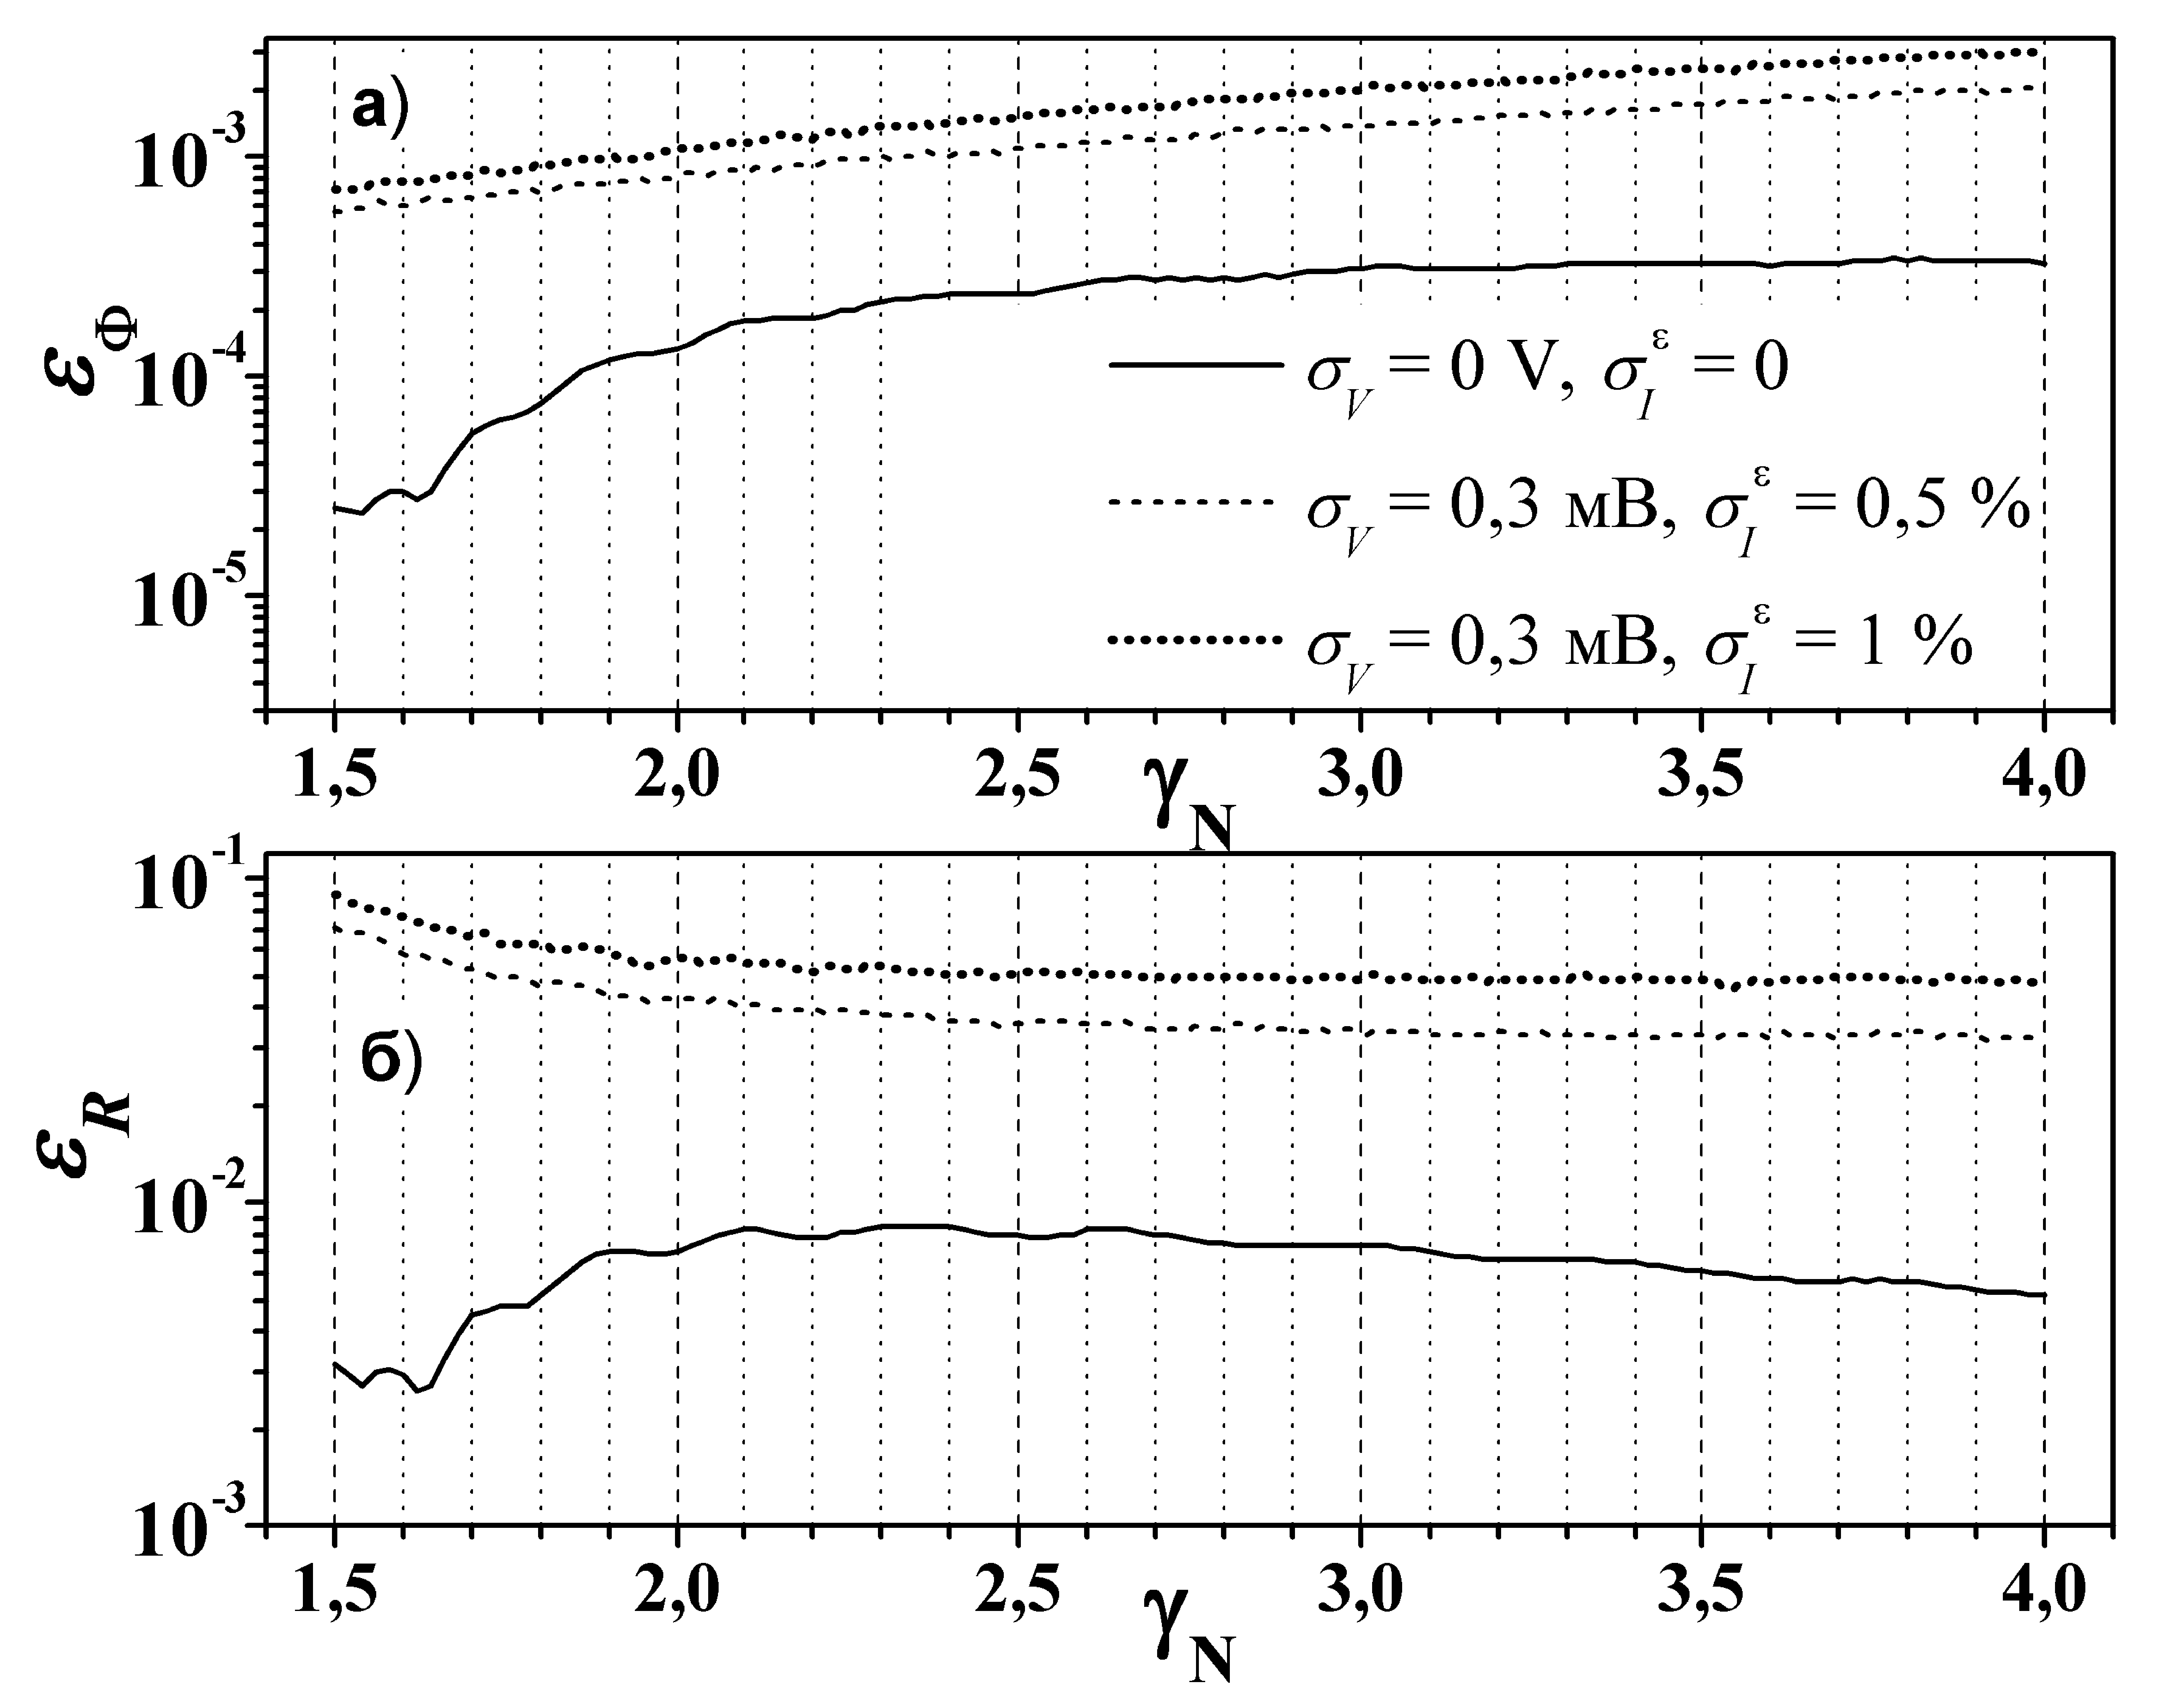
\includegraphics[width=0.6\textwidth]{figNorde}%
\caption{\label{figNorde}
Залежності похибки визначення $\Phi_b$ (a) та $R_s$ (б)  від величини $\gamma_N$.
 при застосуванні метода Норда до набору ідеальних синтезованих ВАХ (суцільні лінії) та зашумлених даних (штрихові лінії)
}
\end{figure}

J.~Werner  \cite{Werner} показав, що за умови коли падіння напруги в області бар'ру $V_d=(V-IR_s)\gg nkT/q$, то
\begin{equation}
\label{eqWerner}
\frac{(dI/dV)}{I}=\frac{q}{nkT}\left[1-R_s\left(\frac{dI}{dV}\right)\right].
\end{equation}
Рівняння~(\ref{eqWerner}) показує, що графік  залежності   $(dI/dV)/I$  від $(dI/dV)$ має бути прямою лінією,
причому її нахил та точка перетину з вертикальною віссю визначаються $R_s$ and $n_\mathrm{id}$.

На жаль, даний метод дозволяє визначити лише два параметри ДШ.
Для оцінки величини ВБШ була використана наступна процедура.
Спираючись на визначене значення $R_s$, експериментальна або синтезована ВАХ корелювалася і проводилась побудова залежності  $\ln I$ від $V_d$.
Після цього проводилась апроксимація отриманої залежності лінійною функцією за методом найменших квадратів \cite[с.~67]{KalitkinBook} в діапазоні $V_d>3kT/q$.
Необхідно підкреслити, що під час апроксимації нахил кривої може розглядатися або як незалежна величина, яка обчислюється, або як відома величина, що визначається попередньо визначеним (під час апроксимації функції (\ref{eqWerner})) значенням $n_\mathrm{id}$.
В роботі розглянуто обидва випадки.
Якщо величини $R_s$ and $n_\mathrm{id}$ визначались шляхом лінійної апроксимації функції (\ref{eqWerner}), а $\Phi_b$ --- як перетин залежності $\ln I=f(V_d)$ при відомому нахилі, то використовується позначення <<Werner>>.
Якщо ж лише $R_s$ визначається за допомогою функції Вернера (\ref{eqWerner}), а $\Phi_b$ and $n_\mathrm{id}$ обчислюються потім із залежності $\ln I=f(V_d)$, то використовується позначення <<Werner*>>.
Подібний підхід до позначень отриманих результатів (із зірочкою та без неї належно від того, скільки незалежних величин використовується при апроксимації скорельованих відповідно до визначеного раніше значення послідовного опору ВАХ) використовуються і для інших методів, детальніше описаних нижче.

R.~Cibils  та R.~Buitrago \cite{Cibils} запропонували використовувати допоміжну функцію у вигляді
\begin{equation}
\label{eqCibils}
F_a(V)=V-V_a\ln I,
\end{equation}
де
$V_a$ практично довільне значення напруги, $V_a\geq99,5I_sR_s+n_\mathrm{id}kT/q$.
Якщо $I_{min,a}$ --- це значення струму, яке відповідає напрузі $V_{min}$, при якій спостерігається мінімум функції $F_a(V)$,
то залежність $I_{min,a}$ від $V_a$ має бути \cite{Cibils} лінійною:
\begin{equation}
\label{eqCibilsDet}
I_{min,a}=(V_a-n_\mathrm{id}kT/q)/R_s\,.
\end{equation}
В роботі при побудові сімейства допоміжних функцій згідно з виразом (\ref{eqCibils}) використовувалися значення  $V_a$ в діапазоні від 0,035~В до максимального значення напруги для даної ВАХ.
Крок зміни $V_a$ дорівнював 1~мВ.
Отримані результати позначені міткою <<Cibils>>.

А.~Kaminski зі співавторами \cite{Kaminski} запропонували два методи.
Перший з них використовує допоміжну функцію, яка будується з використанням інтегрування ВАХ.
Ордината та абсциса $j-$ої точки допоміжного графіку розраховуюся як
\begin{equation}
\label{eqKam1}
Y_j=\frac{1}{I_j-I_1}\int_{V_1}^{V_j}I\,dV \quad\text{and}\quad X_j=\frac{I_j+I_1}{2},
\end{equation}
де
$V_i$ та $I_i$ --- це координати $i-$ої точки ВАХ,
$i\in(1,\ldots, N_p)$,
$j\in(2,\ldots, N_p)$.
Згідно з цим методом очікується, що залежність $Y$ від $X$ має бути лінійною:
\begin{equation}
\label{eqKam1Det}
Y=n_\mathrm{id}kT/q+R_sX.
\end{equation}
Тобто лінійна апроксимація допоміжної функції дозволяє визначити $R_s$ та $n_\mathrm{id}$.

В роботі лінійна апроксимація здійснювалась за допомогою методу найменших квадратів.
Числове інтегрування ВАХ здійснювалось за методом трапецій \cite[с.~98]{KalitkinBook}.
Отримані результаті позначені мітками <<Kaminski I>> та <<Kaminski* I>>.

У другому методі, розглянутому в роботі \cite{Kaminski}, також використовується допоміжна функція $Y$ від $X$, проте
\begin{equation}
\label{eqKam2}
Y_k=\frac{\ln(I_j/I_i)}{I_j-I_i} \quad\text{and}\quad X_k=\frac{V_j-V_i}{I_j-I_i},
\end{equation}
$i\in(1,\ldots, N_p-1)$,
$j\in(i+1,\ldots, N_p)$,
$k\in(1,\ldots, N_p(N_p-1)/2)$.
Отримана таким чином залежність має бути прямолінійною:
\begin{equation}
\label{eqKam2Det}
Y=q(-R_s+X)/n_\mathrm{id}kT.
\end{equation}
Отримані за допомогою даного підходу результати позначені мітками <<Kaminski II>> та <<Kaminski* II>>.

У методі, запропонованому в роботі \cite{Bohlin}, використовуються дві функції Норда, побудовані з використанням двох різних значень $\gamma_N$:
\begin{eqnarray}
\label{eqBohlin}
F_1(V)&=&V/\gamma_1-kT/q\cdot\ln(I/AA^*T^2),
\nonumber\\
F_2(V)&=&V/\gamma_2-kT/q\cdot\ln(I/AA^*T^2).
\end{eqnarray}
Передбачено, що параметри ДШ визначаються за допомогою співвідношень
\begin{eqnarray}
\label{eqBohlinDet}
n_\mathrm{id}&=&\frac{1}{2}\left[\frac{\gamma_1I_{min,2}-\gamma_2I_{min,1}}{I_{min,2}-I_{min,1}}+\right.
\\
&&\left.\frac{V_{min,1}-V_{min,2}+(\gamma_2-\gamma_1)kT/q}{F_2(V_{min,2})-F_1(V_{min,1})-V_{min,2}/\gamma_2+V_{min,1}/\gamma_1}\right]
,\nonumber
\\
Rs&=&\frac{kT}{2q}\left[\frac{\gamma_1-n_\mathrm{id}}{I_{min,1}}+\frac{\gamma_2-n_\mathrm{id}}{I_{min,2}}\right]\,,
\\
\Phi_b&=&\frac{1}{2}\left[F_1(V_{min,1})+\frac{(\gamma_1-n_\mathrm{id})(qV_{min,1}-\gamma_1kT)}{\gamma_1qn_\mathrm{id}}\,+\right.
\nonumber\\
&&\left.F_2(V_{min,2})+\frac{(\gamma_2-n_\mathrm{id})(qV_{min,2}-\gamma_2kT)}{\gamma_2qn_\mathrm{id}}\right].
\end{eqnarray}
де
$[F_1(V_{min,1}), V_{min,1}]$ та $[F_2(V_{min,2}), V_{min,2}]$ --- це координати мінімумів функцій  $F_1(V)$ від $V$ та $F_2(V)$ від $V$, відповідно;
$I_{min,1}$ та $I_{min,2}$ --- значення струму, які відповідають на ВАХ значенням напруги $V_{min,1}$ та $V_{min,2}$, відповідно.

Проведені числові дослідження показали, що, як і в методі Норда, в цьому випадку точність визначення параметрів залежить від вибору величин $\gamma_1$ та $\gamma_2$.
Отримані результати приведені на рис.~\ref{figBohlin}.
Зокрема виявлено, що похибка екстрагування параметрів зростає при збільшенні модуля різниці параметрів $|\gamma_1-\gamma_2|$.
З метою мінімізації помилок методу в подальшому наведені результати, отримані при використанні величин $\gamma_1=1,6$ та $\gamma_2=3,5$.
Отримані результати позначені міткою <<Bohlin>>.

\begin{figure}
\center
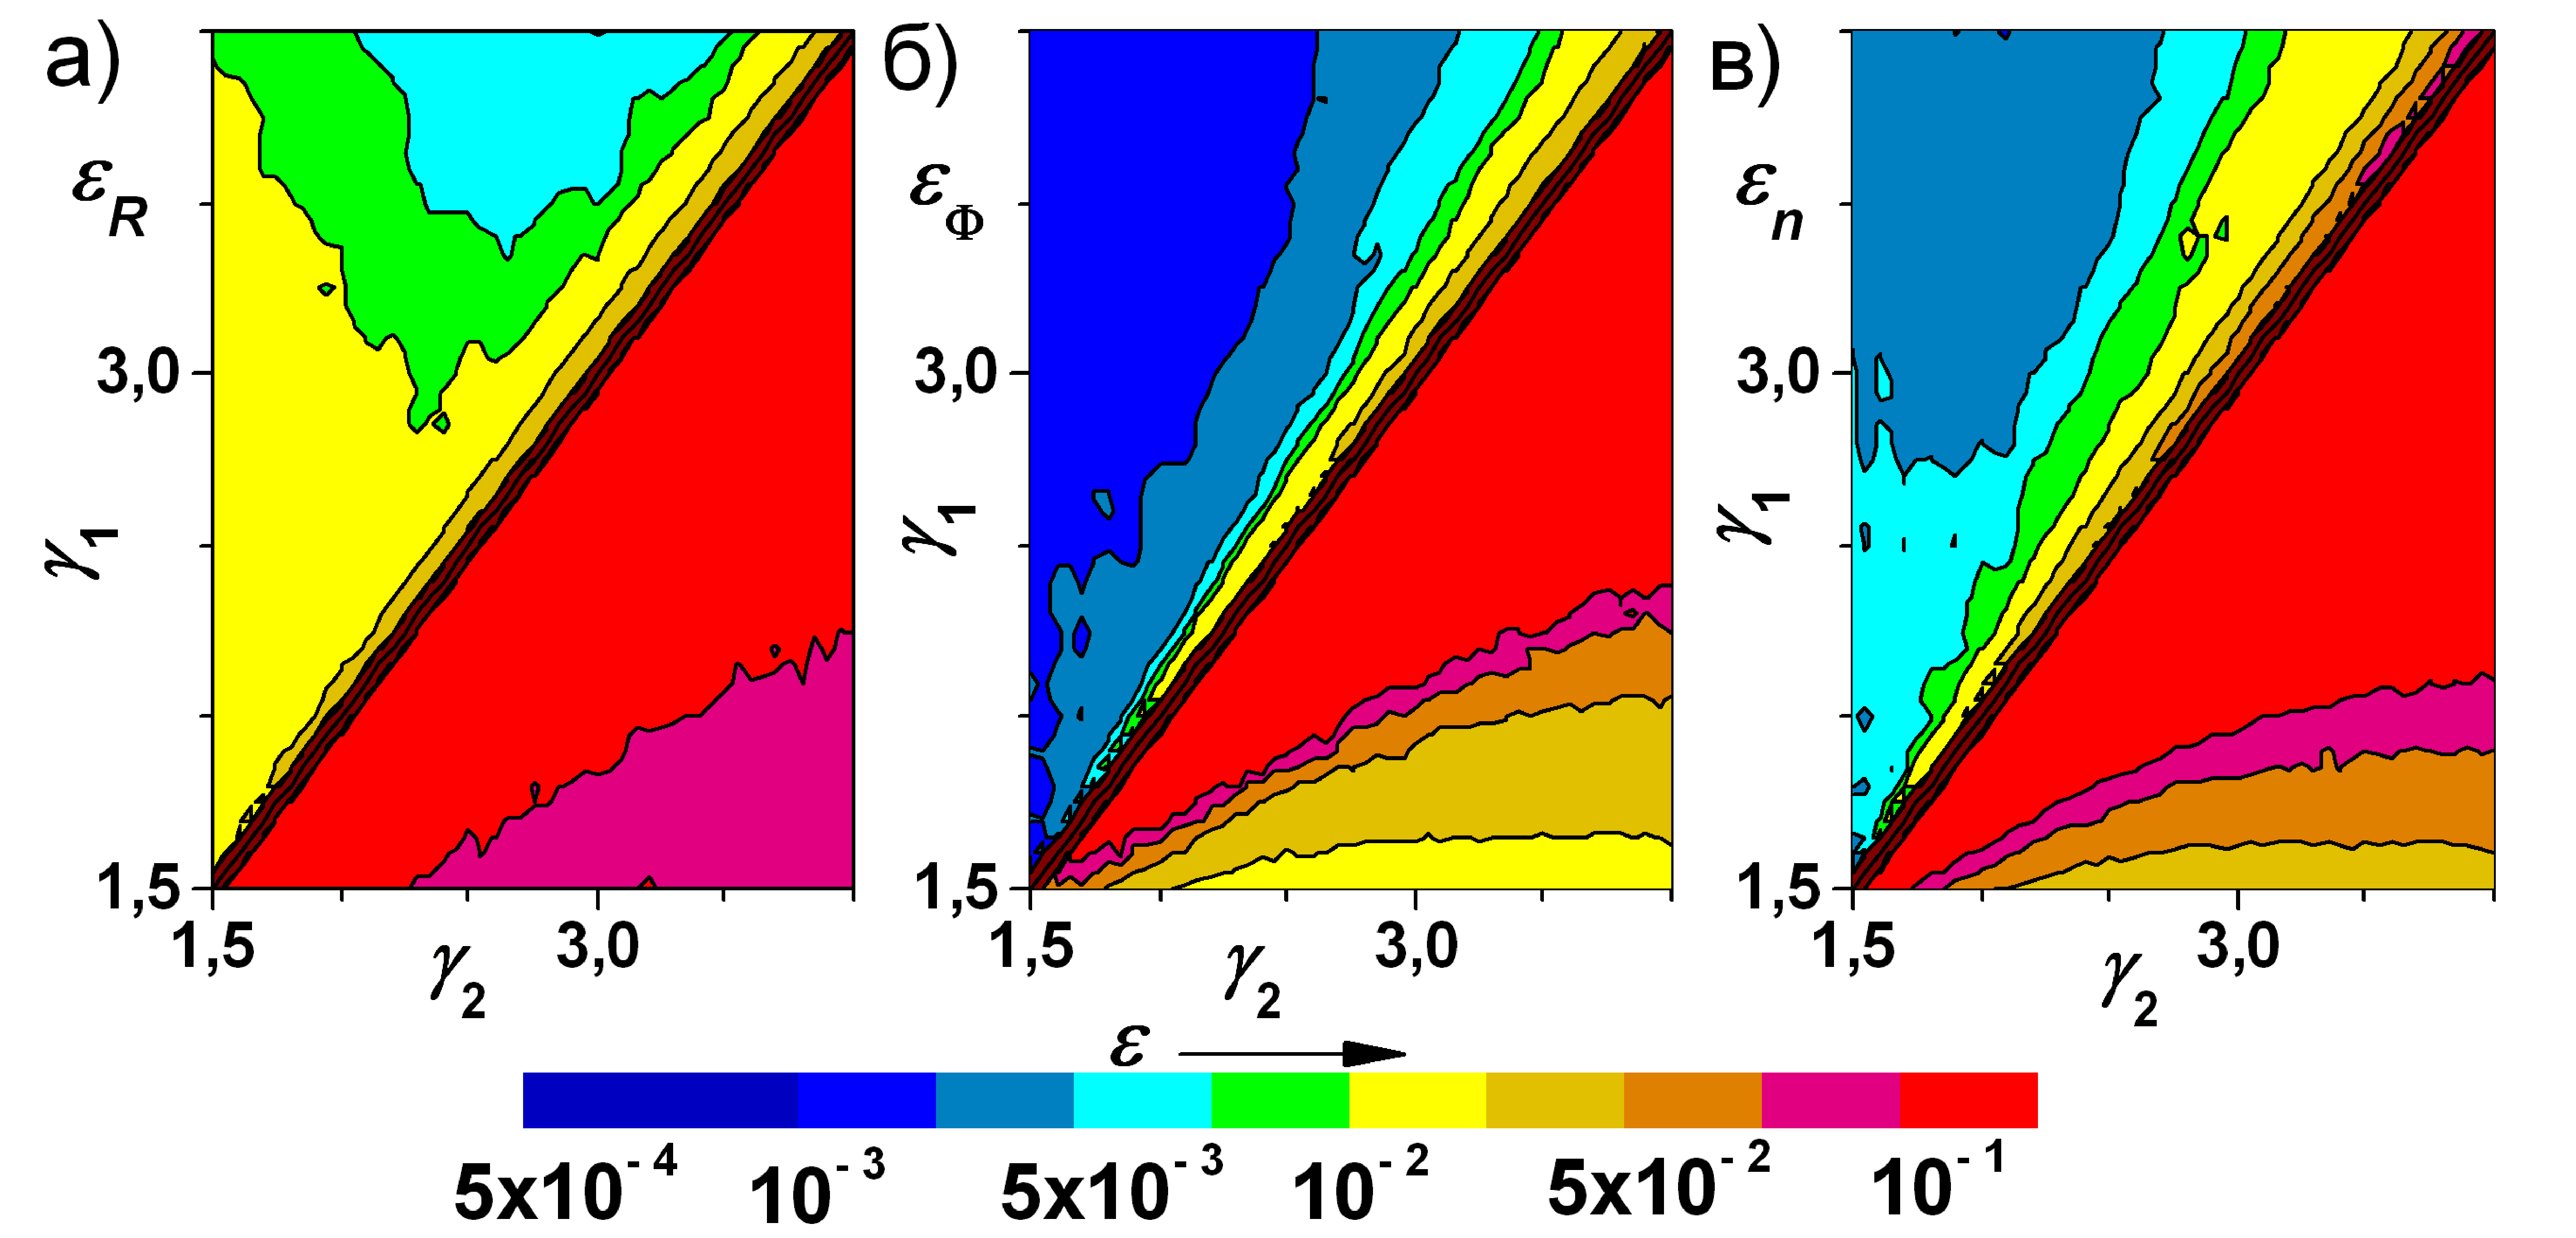
\includegraphics[width=0.8\textwidth]{figBohlin}%
\caption{\label{figBohlin}
Залежності похибок визначення $R_s$ (a), $\Phi_b$ (б) та $n_\mathrm{id}$ (в) від величини параметрів $\gamma_1$ та $\gamma_2$ при застосуванні метода Бохліна.
Наведено результати, отримані для наборів ідеальних ($\sigma_V=0$~V, $\sigma_I^\varepsilon=0$) синтезованих ВАХ (область $\gamma_1>\gamma_2$) та зашумлених ($\sigma_V=0,3$~мВ, $\sigma_I^\varepsilon=1\%$) даних (область $\gamma_2>\gamma_1$)
}
\end{figure}

В роботі \cite{Lee} для визначення параметрів ДШ запропоновано використовувати масив функцій $\{F_L(I)\}$:
\begin{equation}
\label{eqLee}
F_L(I)=V(I)-V_a\ln I,
\end{equation}
де
$V_a$ --- це довільне значення напруги.
Кожна з функцій $F_L(I)$ має бути апроксимована залежністю
\begin{equation}
\label{eqGrFit}
y(I)=c_1+c_2I+c_3\ln I
\end{equation}
та параметри $c_1$, $c_2$ та $c_3$ мають бути визначені.
Тоді очікується \cite{Lee}, що при $V>3kT/q$,
залежність $I_a=-c_3/c_2$ від $V_a$ має бути лінійною:
\begin{equation}
\label{eqLeeDet}
I_a(V_a)=(-n_\mathrm{id}kT/q+V_a)/R_s,
\end{equation}
що дозволяє визначити послідовний опір та фактор неідеальності.
В свою чергу, $\Phi_b$ може бути розрахований \cite{Lee} за допомогою виразу
\begin{equation}
\label{eqLeeFb}
\Phi_b=c_3/n_\mathrm{id}+kT/q\cdot\ln\left(AA^*T^2\right).
\end{equation}

В роботі при застосуванні даного методу використовувалися значення $V_a$ починаючи з 40~мВ з кроком 20~мВ;
апроксимація $F_L(I)$ здійснювалась за методом найменших квадратів.
Отримані дані позначені міткою <<Lee>>.

В роботі Д.~Громова та В.~Пугачевича \cite{Gromov} розглянуто два можливі шляхи визначення параметрів ДШ.
Згідно з першим з них залежність напруги від струму може бути апроксимована виразом (\ref{eqGrFit}) причому
\begin{eqnarray}
\label{eqGr1}
R_s&=&c_2\,,
\\
n_\mathrm{id}&=&(c_3q)/(kT)\,,
\\
\Phi_b&=&\left[c_1/c_3+\ln\left(AA^*T^2\right)\right]kT/q\,.
\end{eqnarray}
Другий шлях полягає у тому, що вираз (\ref{eqGrFit}) застосовується до апроксимації функції Норда з $\gamma_N=2$:
\begin{equation}
\label{eqGr2}
F(I)=V(I)/2-kT/q\cdot\ln(I/AA^*T^2).
\end{equation}
В цьому випадку \cite{Gromov}
\begin{eqnarray}
\label{eqGr2Det}
R_s&=&2c_2\,,
\\
n_\mathrm{id}&=&(2c_3q)/(kT)+2\,,
\\
\Phi_b&=&\frac{2c_1}{n_\mathrm{id}}+\frac{(2-n_\mathrm{id})kT}{n_\mathrm{id}q}\ln\left(AA^*T^2\right)\,.
\end{eqnarray}
Застосування методів показало, що обидва підходи приводять до абсолютно однакових результатів.
Більше того, визначені значення параметрів дуже близькі до даних, які отримані за однакових початкових умов при використанні методу, описаного в роботі \cite{Lee} та згаданого трохи вище.
Тобто ці методи не є незалежними.

З іншого боку, проведені оцінки показали, що точність визначення параметрів за допомогою цих методів залежить від діапазону вихідної ВАХ, який використовується для побудови допоміжної функції, яка потім апроксимується залежністю (\ref{eqGrFit}).
На рис.~\ref{figGromov} наведено залежності похибок екстрагованих параметрів від початкового значення діапазону напруг, в якому проводилась апроксимація.
Видно, що для ідеальних ВАХ точність підвищується при звуженні використаного діапазону.
Водночас для зашумлених даних спостерігається екстремальне значення точності  при певних значеннях ширини діапазону.
Причому ширина та положення діапазону, при якому точність визначення параметрів найбільша, залежить від рівня шуму.



\begin{figure}
\center
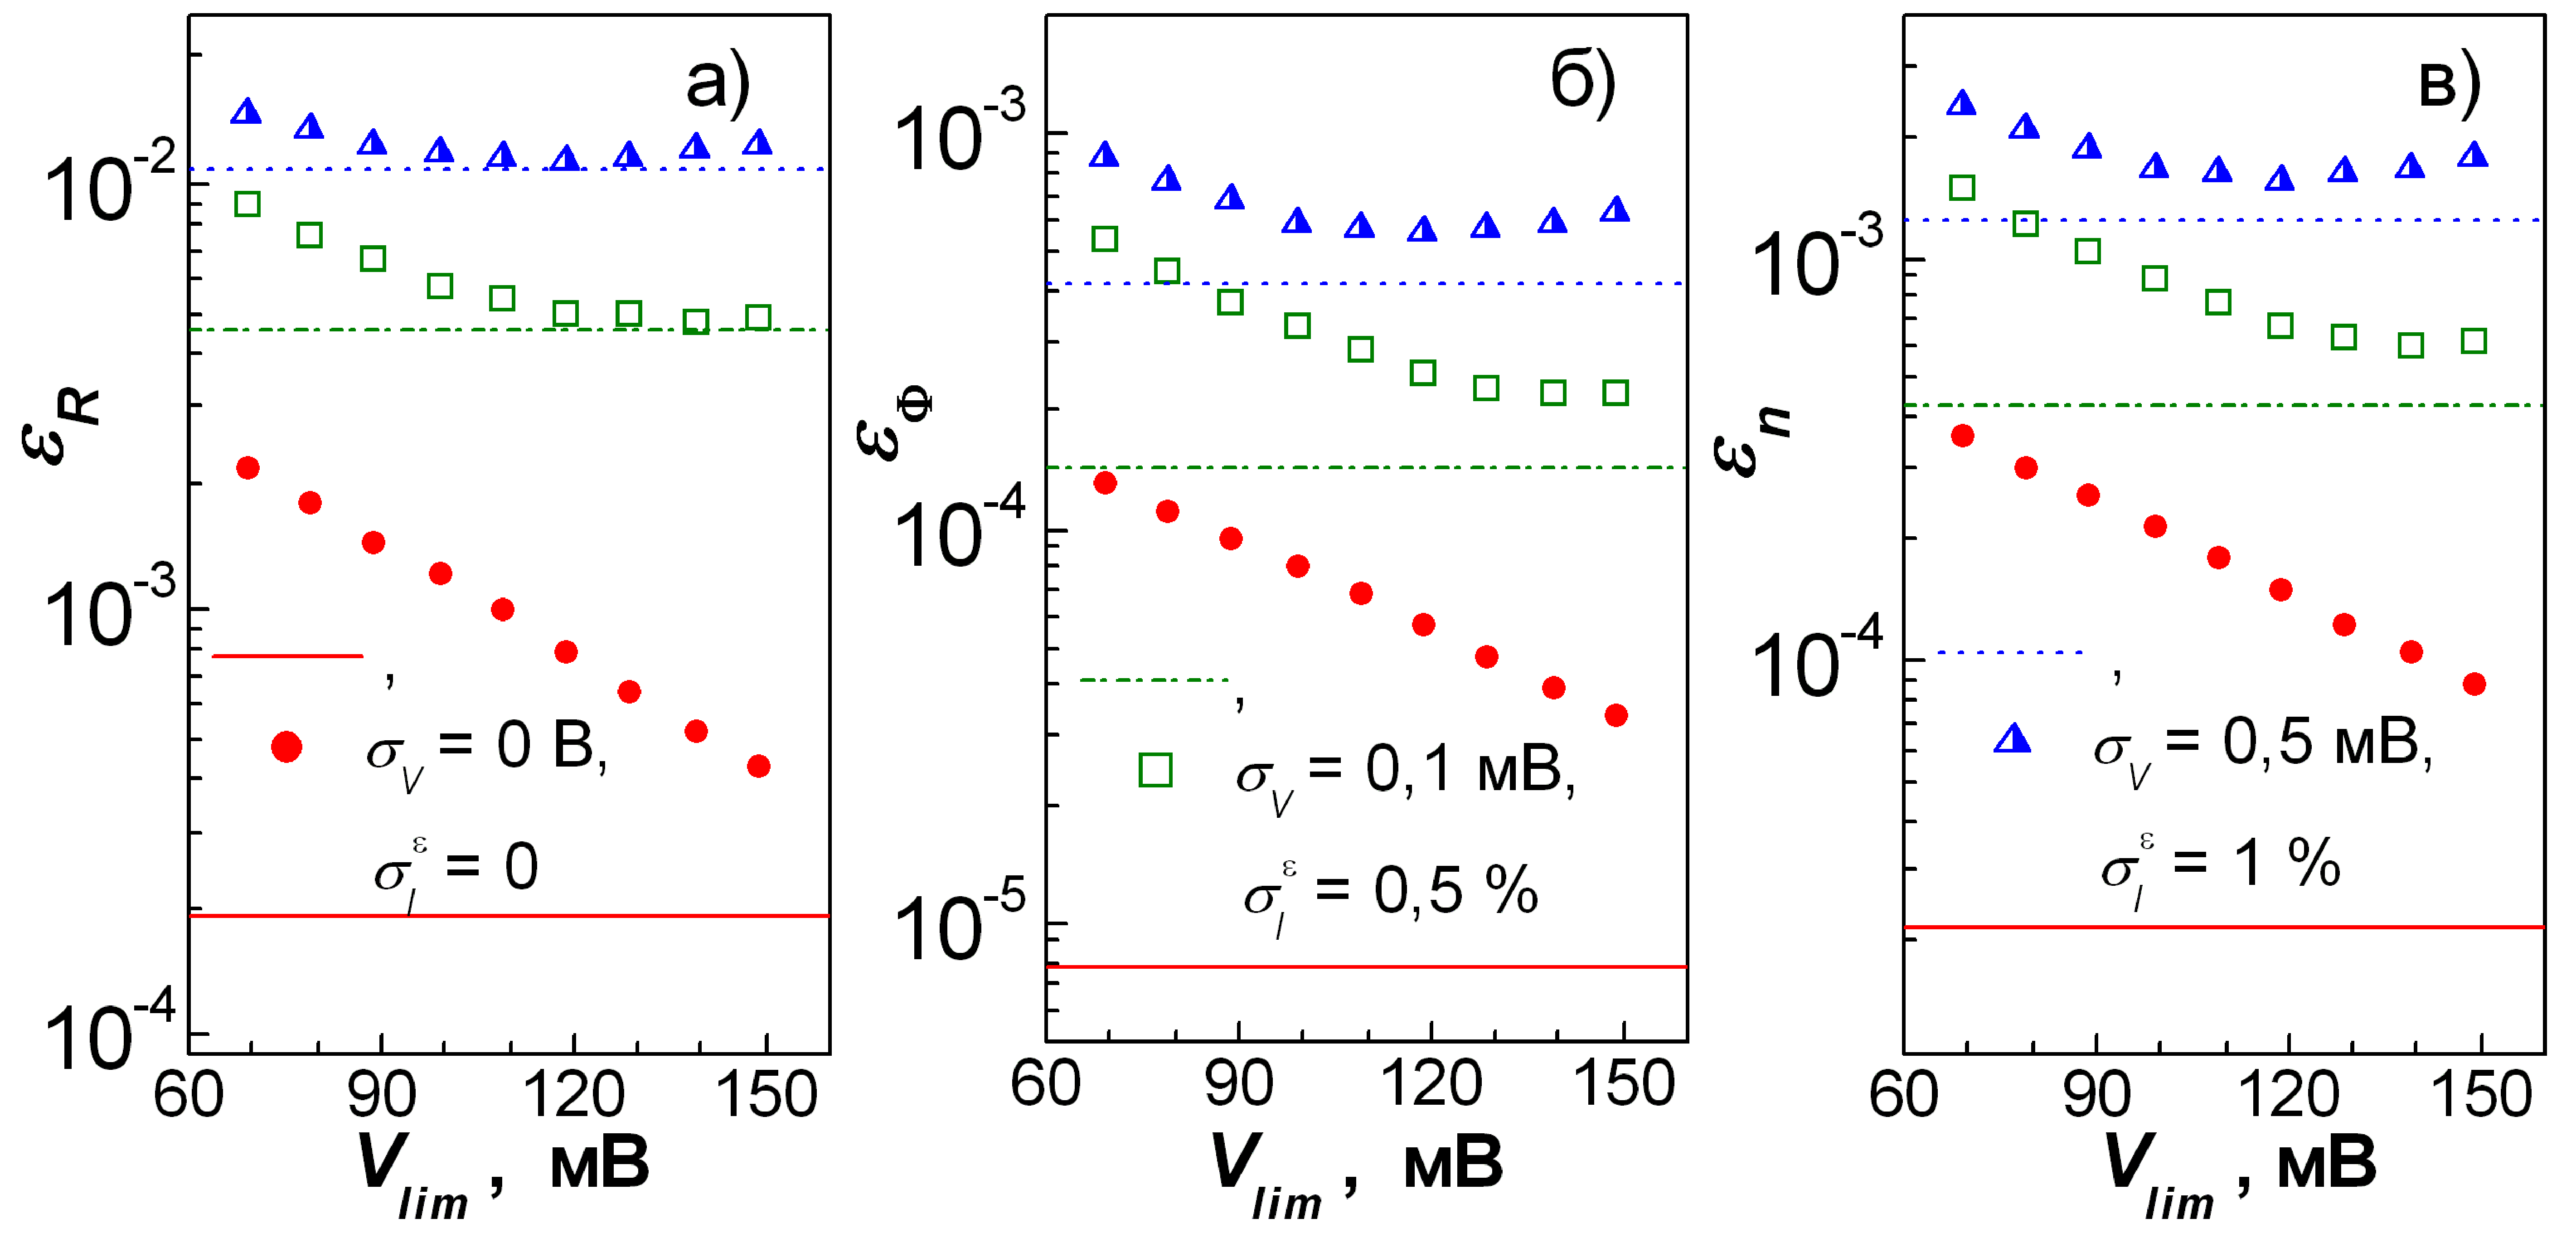
\includegraphics[width=0.9\textwidth]{figGromov}%
\caption{\label{figGromov}
Залежності похибок визначення $R_s$ (a), $\Phi_b$ (б) та $n_\mathrm{id}$ (в) при використанні методу Громова.
Наведено результати, отримані при апроксимуванні залежністю (\ref{eqGrFit}) допоміжної функції, побудованої
на основі ділянки ВАХ в діапазоні напруг від $V_{lim}$ до максимально значення.
Горизонтальні лінії вказують похибки значень параметрів ДШ, які отримані при використанні адаптивної процедури (див. текст).
Представлені результати, отримані при застосуванні методу до ідеальних синтезованих ВАХ (заповнені кружечки, суцільні лінії) та зашумлених даних
з $\sigma_V=0,1$~мВ та $\sigma_I^\varepsilon=0,5\%$ (незаповлені квадрати, штрих--пунктирні лінії) та з $\sigma_V=0,5$~мВ та $\sigma_I^\varepsilon=1\%$
(напівзаповнені трикутники, пунктирні лінії)
}
\end{figure}

У зв'язку з цим, для покращення ефективності роботи методів Громова та Лі, пропонується використовувати спеціальну адаптивну процедуру вибору діапазону побудови допоміжної функції.
Вона полягає в тому, що параметрів визначаються для всіх можливих діапазонів, кількість яких залежить від кількості точок вихідної ВАХ.
Після цього для кожного отриманого набору параметрів обчислюється величина $\theta=\sum_{i=1}^{N_p}[1-I_{calc}(V_i)/I_i]^2$,
де $I_{calc}(V_i)$ розраховується з використанням виразів (\ref{eqSDIV}) та (\ref{eqSDIs}).
Найкращим за точністю вважається той набір параметрів, для якого спостерігається мінімум величини $\theta$.

Зрозуміло, що подібна адаптивна процедура збільшує час, необхідних для визначення параметрів ДШ через необхідність багатократного повторення застосування методу Громова (Лі) та додаткових розрахунків.
Проте, з іншого боку, ця процедура може бути автоматизована, а також дозволяє підвищити точність (лінії на рис.~\ref{figGromov}).

Нижче представлені результати застосування методу Громова з використанням запропонованої адаптивної процедури.
Отримані дані позначені міткою <<Gromov>>.
Різниця між ними та позначеними міткою <<Lee>> визначає, фактично, доцільність запропонованої процедури.

В роботі \cite{Cheung} запропоновано визначати параметри ДШ шляхом побудови залежностей функцій $H(V)$
\begin{equation}
\label{eqH}
H(I)=V-\frac{n_\mathrm{id}kT}{q}\ln\left(\frac{I}{AA^*T^2}\right).
\end{equation}
та $dV/d(\ln I)$ від сили струму.
За умови $V_d>3kT/q$ ці залежності мають бути лінійними, причому
\begin{eqnarray}
\label{eqChung}
\frac{dV}{d\ln I}&=&R_sI+n_\mathrm{id}kT/q,
\\
\label{eqHDet}
H(I)&=&n_\mathrm{id}\Phi_b+IR_s.
\end{eqnarray}
При застосуванні методу спочатку визначаються $R_s$ та  $n_\mathrm{id}$ на основі рівняння (\ref{eqChung}),
а потім  $\Phi_b$, використовуючи вираз~(\ref{eqHDet}) та обчислене на попередньому кроці значення $n_\mathrm{id}$.
Отримані результати позначені міткою <<Chung>>.

Ще одним методом, де використовуються диференційні коефіцієнти ВАХ, є запропонований в роботі \cite{Mikhelashvili}.
В цьому випадку все починається з обчислення функції  $\alpha(V)$:
\begin{equation}
\label{eqMikh}
\alpha(V)=d(\ln I)/d(\ln V).
\end{equation}
Визначення параметрів відбувається з використанням співвідношень
\begin{eqnarray}
\label{eqMikhDet}
R_s&=&\frac{V_{max}}{\alpha^2_{max}I_{max}}\,,
\\
n_\mathrm{id}&=&\frac{qV_{max}(\alpha_{max}-1)}{\alpha_{max}^2kT}\,,
\\
\Phi_b&=&\frac{kT}{q}\left[\alpha_{max}+1-\ln\left(\frac{I_{max}}{AA^*T^2}\right)\right]\,.\label{eqMikhDetFi}
\end{eqnarray}
де
$\alpha_{max}$ та $V_{max}$  це координати максимуму залежності $\alpha$ від $V$;
$I_{max}$ --- сила струму, яка відповідає напрузі $V_{max}$.

\begin{figure}
\center
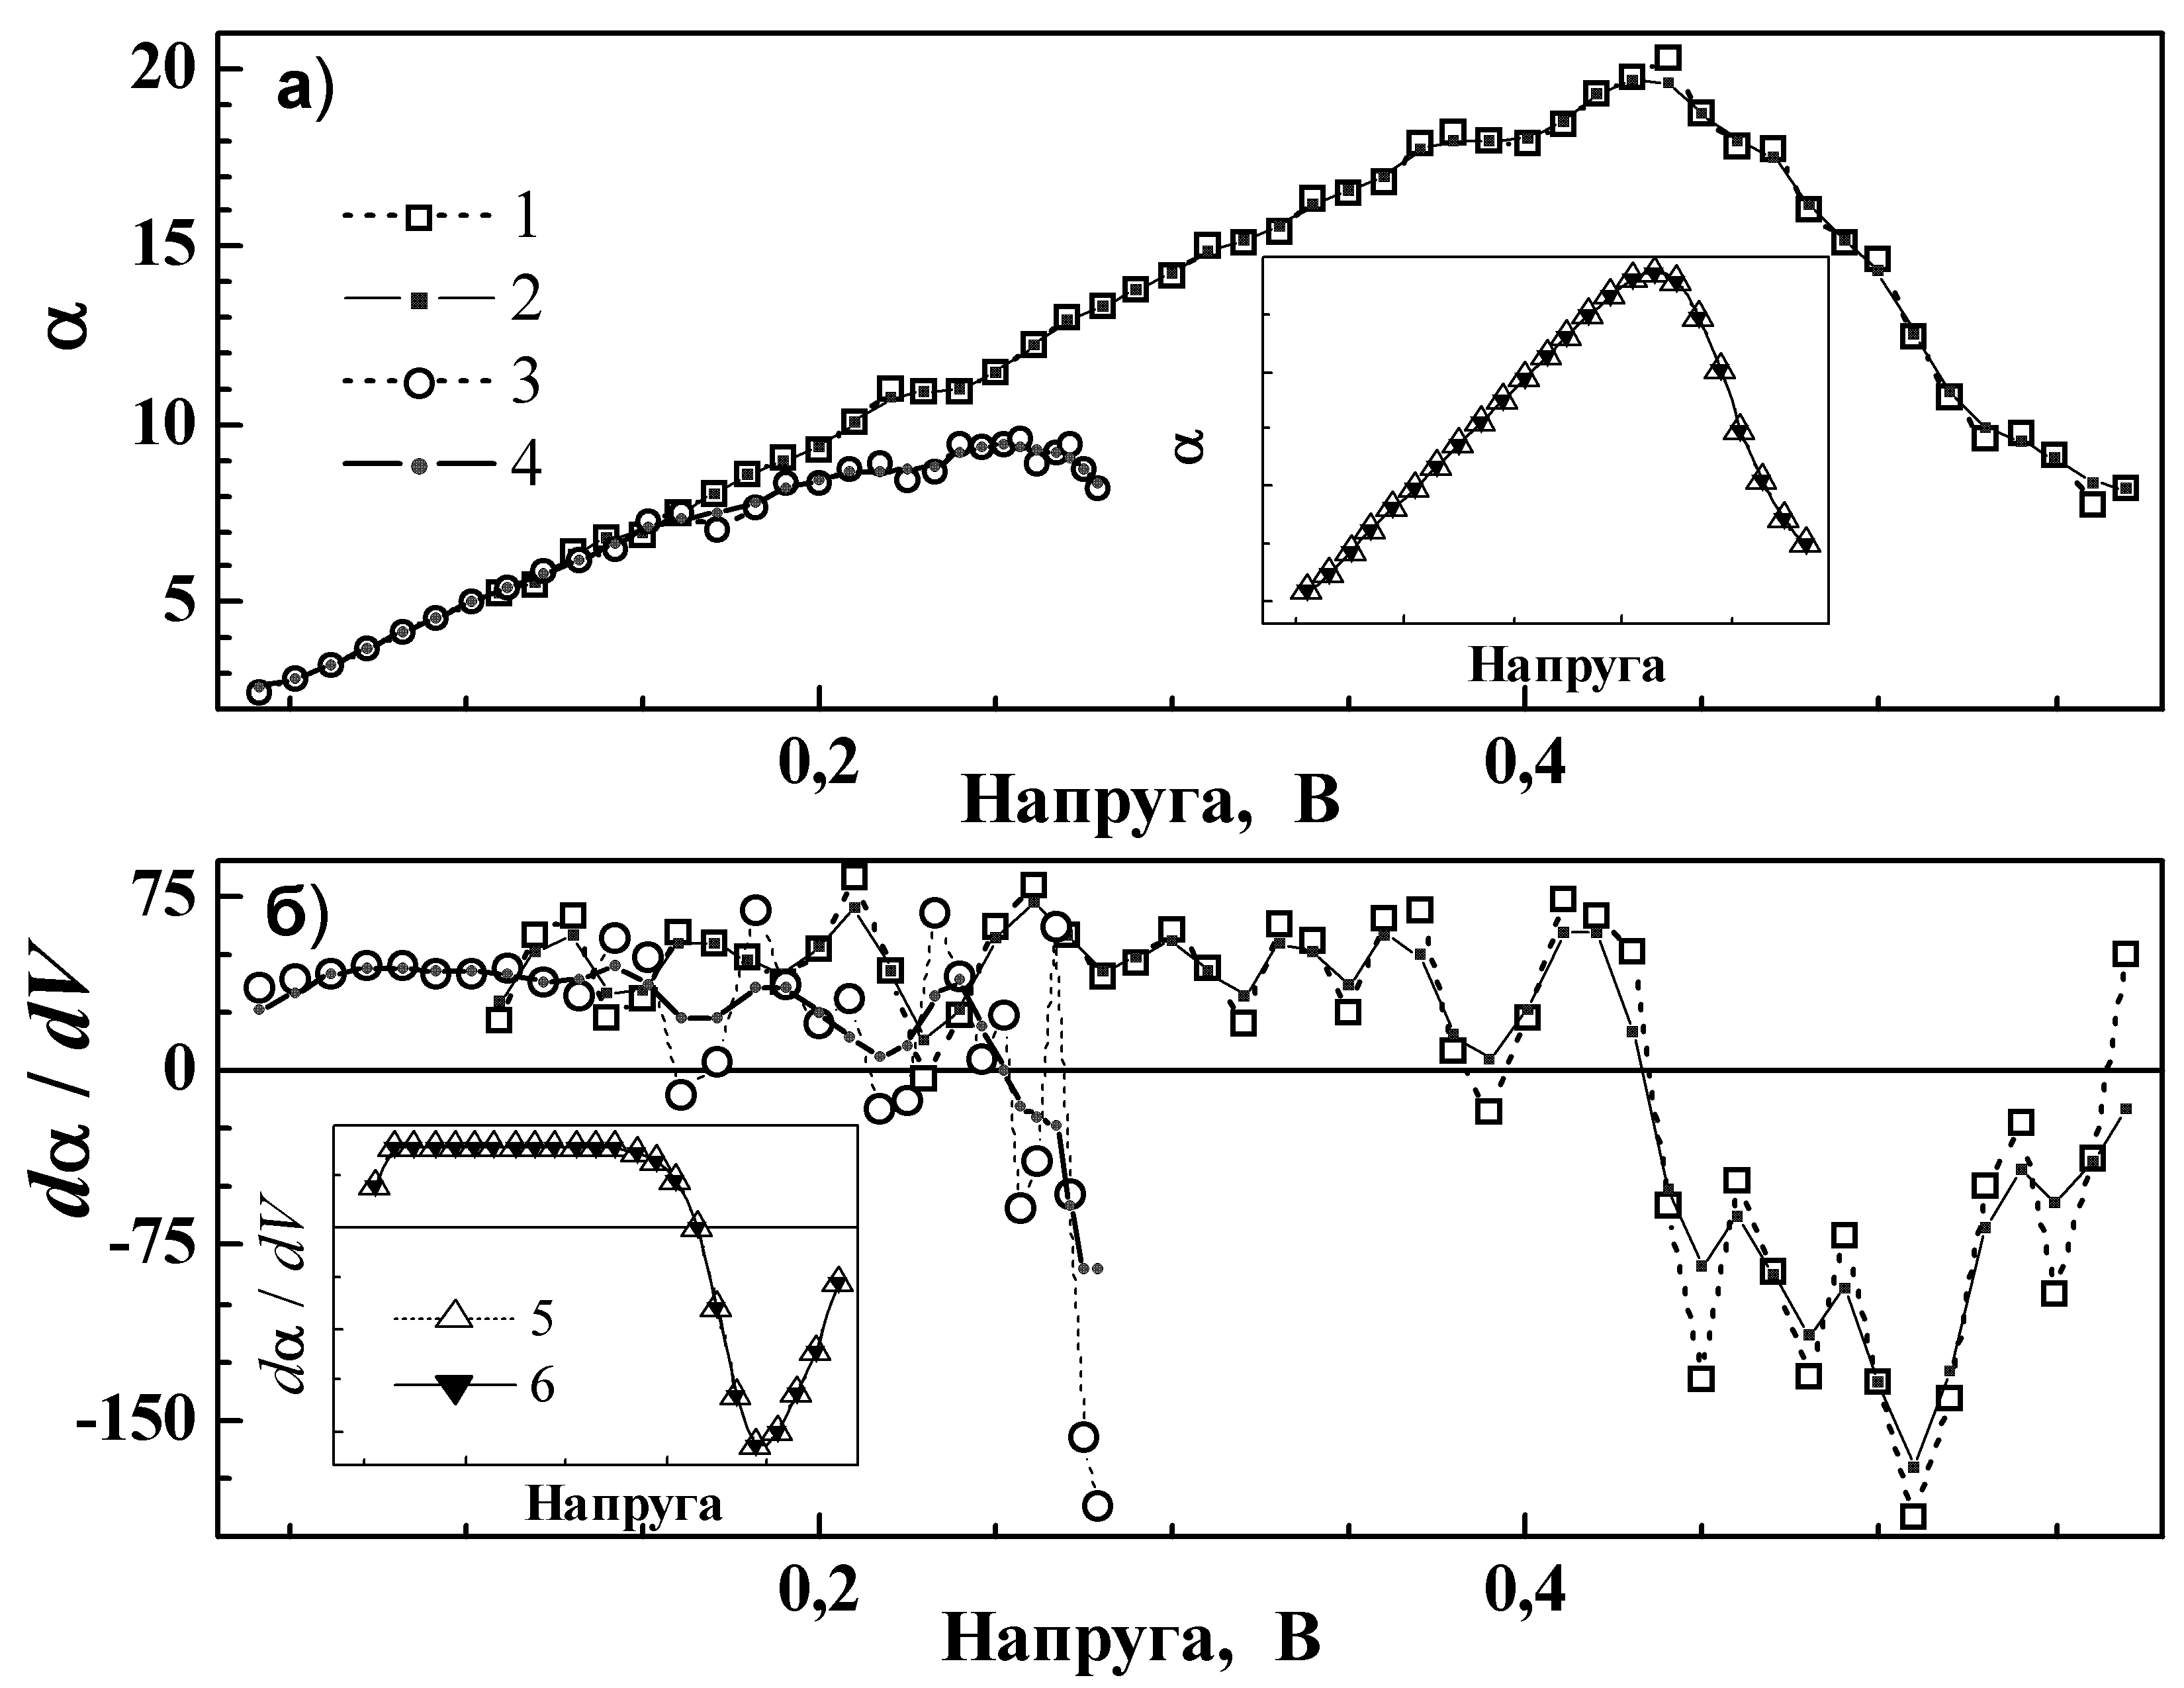
\includegraphics[width=0.65\textwidth]{figMikh}%
\caption{\label{figMikh}
Залежності функції~(\ref{eqMikh}) (а) та її похідної (б) від напруги.
Наведено графіки для зашумлених даних ($\sigma_V=0,3$~мВ, $\sigma_I^\varepsilon=1\%$, криві 1 та 2), для експериментально виміряних ВАХ (криві 3 та 4) та для ідеальних синтезованих ВАХ (вставка, криві 5 та 6) до (1, 3, 5) та після (2, 4, 6) запропонованої обробки
}
\end{figure}

Зауважимо, що однією з необхідних властивостей методу, які використовуються для обчислення параметрів пристроїв з набору ВАХ, отриманих за різних умов, є можливість його застосування в автоматичному режимі.
В цьому випадку один з найпоширеніших варіантів пошуку екстремуму полягає у знаходженні нулів похідної.
Як видно з виразів (\ref{eqMikh})--(\ref{eqMikhDetFi}), для даного методу це означає необхідність проведення процедури числового визначення другої похідної ВАХ.


Рис.~\ref{figMikh}(a) показує, що при використанні експериментальних ВАХ чи зашумлених даних числове диференціювання викликає появу багаточисленних локальних екстремумів на залежності функції $\alpha$ від $V$.
Ці екстремуми заважають автоматичному виявленню точки максимуму через наявність багатьох нульових точок на залежності $d\alpha/dV$ від $V$ (рис.~\ref{figMikh},б).
З метою подолання цих труднощів, в роботі запропоновано проводити спеціальну 2-стадійну процедуру обробки даних.
А саме, на першій стадії обробки до отриманої з ВАХ залежності $\alpha$ від $V$ пропонується застосовувати 3--точковий медіанний фільтр, після чого, на другій стадії, проводити згладжування.
І лише після цього, проводити визначення положення максимуму, визначення величин $\alpha_{max}$, $V_{max}$  та $I_{max}$ і розрахунок величин параметрів ДШ.
Дані на рис.~\ref{figMikh} показують, що запропонована процедура обробки дійсно зменшує вплив побічних максимумів та дозволяє покращити точність методу.
Згладжування здійснюється завдяки усередненню по трьом сусіднім точкам з ваговими коефіцієнтами, які визначаються розподілом Гауса з дисперсією, рівною 0,6.

Надалі наведено результати, позначені міткою <<Mikhelashvili>> та отримані з використанням зазначеної процедури обробки.


\subsection{Числові методи}
Надалі також наведені результати отримані при використанні стандартного методу найменших квадратів зі статистичними ваговими коефіцієнтами \cite[с.~67]{KalitkinBook}.
В цьому випадку параметри визначались шляхом мінімізації квадратичної форми
\begin{equation}
\label{eqLS}
S(I_s,n_\mathrm{id},R_s)=\sum_{i=1}^{N_p}I_i^{-1}\left[I_i-I_{calc}(V_i,I_s,n_\mathrm{id},R_s)\right]^2,
\end{equation}
де $I_{calc}$ --- значення сили струму, отримане при інтерполяції.
При мінімізації шукався розв'язок системи рівнянь, отриманих з умов $\partial S/\partial I_s=0$,
$\partial S/\partial n_\mathrm{id}=0$ та $\partial S/\partial R_s=0$.
Пошук розв'язку цієї системи нелінійних рівнянь проводився за допомогою методу покоординаткого градієнтного спуску \cite[с.~231]{KalitkinBook}.
Як критерій зупинки ітераційного процесу було вибрано умову $\mid(S_j-S_{j+1})/S_j\mid<10^{-12}$,
де $S_j$ --- це значення квадратичної форми на $j-$му кроці ітерації.
Початкове наближення величини $R_s$ обчислювалося шляхом визначення перетину з координатною віссю залежності $(dV/dI)/I$ від $1/I$,
побудованої з використанням останніх п'яти точок ВАХ.
Початкові наближення $I_s$ та $n_\mathrm{id}$ отримувалися шляхом лінійної апроксимації залежності $\ln I$ від $V_d$, причому для визначення останньої величини використовувалися початкове наближення  $R_s$.

Було розглянуто два варіанти методу найменших квадратів.
В першому з них для обчислення $I_{calc}$ використовувався вираз ~(\ref{eqSDIV}), тобто квадратична форма мала вигляд
\begin{equation}
\label{eqLSOrd}
S(I_s,n_\mathrm{id},R_s)=\sum_{i=1}^{N_p}I_i^{-1}\left[I_i-I_s\left\{\exp\left[\frac{q(V_i-I_iR_s)}{n_\mathrm{id}kT}\right]-1\right\}\right]^2.
\end{equation}
Отримані внаслідок мінімізації функції~(\ref{eqLSOrd}) результати позначені міткою <<Ordinary LS>>.

В другому випадку при побудові квадратичної форми використовувалася $W$--функція Ламберта.
За визначенням, функція $W$ є розв'язком рівняння $z=W(z)\cdot\exp(W(z))$, її значення обчислюються за допомогою ряду \cite{LambertBook}.
Згідно з результатами, представленими в роботі \cite{Lambert_Jung}, явний розв'язок  трансцендентного рівняння~(\ref{eqSDIV}) може бути виражений за допомогою основної гілки функції Ламберта, причому у випадку нехтування впливом шунтуючого опору він має вигляд
\begin{equation}
\label{eqLam}
    I(V)=\frac{n_\mathrm{id}kT}{qR_s}W\left\{\frac{qR_s}{n_\mathrm{id}kT}
      \exp\left[\frac{q(V+R_sI_s)}{n_\mathrm{id}kT}\right]  \right\}+I_s.
\end{equation}
Тобто квадратична форма може бути записана у вигляді
\begin{equation}
\label{eqLSLamb}
S(I_s,n_\mathrm{id},R_s)=\sum_{i=1}^{N_p}I_i^{-1}\left[I_i-\frac{n_\mathrm{id}kT}{qR_s}W\left\{\frac{qR_s}{n_\mathrm{id}kT}
      \exp\left[\frac{q(V_i+R_sI_s)}{n_\mathrm{id}kT}\right]  \right\}-I_s\right]^2,
\end{equation}
Результати, отримані при мінімізації (\ref{eqLSLamb}), позначені міткою <<Lambert LS>>.


\subsection{Еволюційні алгоритми\label{subEA}}
Еволюційні алгоритми -- це клас обчислювальних оптимізаційних моделей, які при своїй побудові та реалізації імітують поведінку живої природи.
При своїй роботі вони оперують наборами (популяціями) $P$ можливих розв'зків
$\overrightarrow{X}$: $P=\left\{\overrightarrow{X_k}\right\}$, $k\in(1,\ldots, N_S)$,
де $N_S$ --- це загальна кількість розв'язків у популяції.
Кожний із розв'язків (претендентів на звання остаточного розв'язку) є вектором, що складається з дійсних чисел:
$\overrightarrow{X_k}=\left\{x_{k,i}\right\}$, $i\in(1,\ldots, N_D)$,
де
$N_D$ дорівнює загальній кількості параметрів, які слід оптимізувати.
В нашому випадку $N_D=3$, $\overrightarrow{X}=\left\{R_s\,,\,n_\mathrm{id}\,,\,\ln I_s\right\}$.

Перед початком оптимізаційного процесу створюється початкова популяція.
Зазвичай початкові значення параметрів вибираються випадковим чином з інтервалу
$[\overrightarrow{X}^{L}, \overrightarrow{X}^{H}]$:
\begin{equation}
\label{eqEAIn}
x_{k,i,0}=x_i^L+r_{[0,1]}(x_i^H-x_i^L),
\end{equation}
де
$r_{[0,1]}$ --- випадкове число, рівномірно розподілене на інтервалі $[0,1]$,
$\overrightarrow{X}^{L}=\left\{x_i^L\right\}$ та $\overrightarrow{X}^{H}=\left\{x_i^H\right\}$ ---
нижня та верхня границі простору, де шукаються розв'язки, відповідно.
В даній роботі проводився пошук у просторі, границі якого задані наступним чином:
$R_s\in[0,\,50]$~Ом, $n_\mathrm{id}\in[1,\,2]$, $I_s\in[10^{-26},\,10^{-2}]$~A.

На кожному кроці ітерації
а)~проводиться трансформація кожного з розв'язків:
$\left\{\overrightarrow{X_{k}}_{,j-1}\right\}\rightarrow\left\{\overrightarrow{X_{k}}_{,j}\right\}$,
$j\in(1,\ldots, N_{it})$,
$N_{it}$ --- максимальна кількість ітерацій;
процедура трансформації залежить від конкретного алгоритму і описана далі;
б)~розраховується значення функції придатності (або цільової функції) $Fit(\overrightarrow{X_k}_{,j})$
для кожного $k$--го розв'язку.
Оптимальним для $j$--го ітераційного кроку розв'язком $\overrightarrow{X}_{j}^{opt}$ вважається той, для якого
значення функції придатності мінімальне:
$Fit(\overrightarrow{X}_{j}^{opt})=min\left\{Fit(\overrightarrow{X_k}_{,j})\right\}$.
Кінцевим результатом вважається $\overrightarrow{X}_{N_{it}}^{opt}$.

В даній роботі використовувалася цільова функція у вигляді суми квадратів відносних похибок апроксимації кожної з точок ВАХ
\begin{equation}
\label{eqEAFit}
Fit=\sum_{i=1}^{N_p}\left\{1-\frac{I_s}{I_i}\left[\exp\left(\frac{q(V_i-I_iR_s)}{nkT}\right)-1\right]\right\}^2.
\end{equation}
$N_{it}$ визначалося умовою збіжності розв'язку.

Метод диференційної еволюції імітує процеси природного відбору і використовує процеси диференційної мутації та випадкового схрещування.
У термінології даного алгоритму кожний з розв'язків називається особою, а послідовність дій на $j$--му ітераційному кроці має наступний вигляд \cite{DEWang,DEModif}:
\begin{itemize}[leftmargin=0cm,itemindent=1em]
  \item Мутація. Для кожного вектору $\overrightarrow{X_{k}}_{,j-1}$ генерується вектор мутації $\overrightarrow{M_{k}}_{,j}$
  \begin{equation}
 \label{eqDEMut}
 \overrightarrow{M_{k}}_{,j}=\overrightarrow{X_{r_1}}_{,j-1}+F_{sc}\cdot\left(\overrightarrow{X_{r_2}}_{,j-1}-\overrightarrow{X_{r_3}}_{,j-1}\right),
 \end{equation}
 де $r_1,r_2,r_3\in(1,\ldots,N_S)$ вибираються випадковим чином і мають відрізнятися від індексу $k$.
 $F_{sc}\in[0,2]$  --- дійсна стала величина, що називається масштабним коефіцієнтом.


  \item Схрещування. Формується пробний вектор $\overrightarrow{U_{k}}_{,j}$
  \begin{equation}
 \label{eqDECros}
 u_{k,i,j}=\left\{
 \begin{array}{ll}
 m_{k,i,j},& \text{if} \quad r_{[0,1]}\leq C\!R \quad \text{or} \quad i=r_{4}\\
 x_{k,i,j-1},& \text{otherwise}
 \end{array}
 \right.
 \end{equation}
 причому випадкова величина $r_4\in(1,\ldots,N_D)$
забезпечує наявність в $\overrightarrow{U_{k}}_{,j}$ хоча б одного елемента з $\overrightarrow{M_{k}}_{,j}$;
 константа $C\!R\in[0,1]$ називається темп схрещування.
  Спираючись на результати, представлені в \cite{P-DE_Ishaque},
  в даній роботі в даній роботі були використана штрафна функція, яка запобігає виходу розв'язків за межі пошукового простору.
  А саме, будь--який параметр, значення якого перевищувала допустимі межі, замінювався випадковою величиною згідно з
    \begin{equation}
 \label{eqDEPen}
 u_{k,i,j}=\left\{
 \begin{array}{ll}
 u_{k,i,j}-r_{[0,1]}(x_i^H-x_i^L),& \text{if} \quad u_{k,i,j}>x_i^H\\
 u_{k,i,j}+r_{[0,1]}(x_i^H-x_i^L),& \text{if} \quad u_{k,i,j}<x_i^L.
 \end{array}
 \right.
 \end{equation}
  \item Відбір.
      \begin{equation}
 \label{eqDESel}
 \overrightarrow{X_{k}}_{,j}=\left\{
 \begin{array}{ll}
\overrightarrow{U_{k}}_{,j},& \text{if} \quad Fit(\overrightarrow{U_k}_{,j})<Fit(\overrightarrow{X_k}_{,j-1})\\
 \overrightarrow{X_{k}}_{,j-1},& \text{otherwise}.
 \end{array}
 \right.
 \end{equation}

\end{itemize}
Користуючись результатами, представленими в \cite{DEWang},
були вибрані значення $F_{sc}=0,8$, $C\!R=0,3$ та $N_S=8N_D=24$.
Виявлено, що збіжність результатів досягається при $N_{it}=600$.
Отримані результати позначені міткою <<DE>>.

Розвиток методу оптимізації зграї частинок пов'язаний зі спостереженням соціальної поведінки тварин на кшталт зграї птахів чи риб.
У термінології алгоритму PSO розв'язки називаються частинками, які летять (чи плавають) і гіперпросторі параметрів.
На $j$--му ітераційному кроці виконуються наступні дії \cite{PSO_Ye}:
\begin{itemize}[leftmargin=0cm,itemindent=1em]
  \item Визначається найкраще положення $\overrightarrow{X_k}_{,j}^{best}$ для кожної з частинок:
 \begin{equation}
 \label{eqPSO_PB}
 \overrightarrow{X_k}_{,j}^{best}=\left\{
 \begin{array}{ll}
 \overrightarrow{X_k}_{,j-1}^{best},& \text{if} \quad Fit(\overrightarrow{X_k}_{,j-1})\geq Fit(\overrightarrow{X_k}_{,j-1}^{best})\\
 \overrightarrow{X_{k}}_{,j-1},& \text{otherwise}.
 \end{array}
 \right.
 \end{equation}
  \item  Визначається глобально найкраща позиція $\overrightarrow{B}_{j}$ серед всіх частинок зграї:
 \begin{equation}
 \label{eqPSO_GB}
 \overrightarrow{B}_{j}=min\{ Fit(\overrightarrow{X_1}_{,j}^{best}),\ldots, Fit(\overrightarrow{X_{N_S}}_{,j}^{best})\}.
 \end{equation}
  \item Змінюється вектор швидкості кожної частинки
\begin{eqnarray}
 \label{eqPSO_Vel}
\upsilon_{k,i,j}&=&w_j\,\upsilon_{k,i,j-1}+l_1r_{[0,1],1}\cdot(x_{k,i,j}^{best}-x_{k,i,j-1})+
\nonumber\\
&&l_2r_{[0,1],2}\cdot(b_{i,j}-x_{k,i,j-1})
\,,
\end{eqnarray}
де
$l_1$ та $l_2$ називаються коефіцієнти навчання, $w_j$ --- інерційна маса.
У даній роботі, використано підхід лінійного збільшення маси:
 \begin{equation}
 \label{eqPSO_W}
 w_j=w_{max}-j(w_{max}-w_{min})/N_{it},
 \end{equation}
де
$w_{max}$ та $w_{min}$ --- початкова та кінцева маси, відповідно.
Після цього швидкість кожної з частинок оновлюється з використанням наступного виразу:
 \begin{equation}
 \label{PSO_Vmax}
 \upsilon_{k,i,j}=\left\{
 \begin{array}{ll}
 \upsilon_{i}^{max},& \text{if} \quad \upsilon_{k,i,j}>\upsilon_{i}^{max}\\
 -\upsilon_{i}^{max},& \text{if} \quad \upsilon_{k,i,j}<-\upsilon_{i}^{max}\\
 \upsilon_{k,i,j},& \text{otherwise}\,,
 \end{array}
 \right.
 \end{equation}
де
константа $ \overrightarrow{\upsilon}^{max}$  призначена стримувати надлишкові блукання частинок.
Зазвичай \cite{PSO_Ye} $ \overrightarrow{\upsilon}^{max}$ вибирається рівним максимально можливому відхиленню даної частинки в певному напрямі.
 \item Кожна частинка переміщується у нове положення:
 \begin{equation}
 \label{eqPSO_Final}
 \overrightarrow{X_{k}}_{,j}=\overrightarrow{\upsilon_{k}}_{,j}+\overrightarrow{X_{k}}_{,j-1},
 \end{equation}
\end{itemize}
Згідно з \cite{PSO_Ye} було використано наступні значення параметрів:
$l_1=l_2=2$, $w_{max}=0,9$, $w_{min}=0,4$ та $N_S=15N_D=45$.
Крім того, при розрахунках вважалося, що початкові швидкості $\overrightarrow{\upsilon_{k}}_{,0}=0$.
Виявлено, що збіжність результатів досягається при $N_{it}=700$.
Отримані результати позначені міткою <<PSO>>.

Алгоритм методу модифікованої штучної бджолиної сім'ї базується на поведінці рою медоносних бджіл, пов'язаній з пошуком їжі.
Бджоли поділяються на три категорії: носії, спостерігачі та розвідники.
Носії експлуатують свої джерела їжі та взаємодіють зі спостерігачами.
Спостерігачі очікують у вулику та вирішують яке з джерел їжі експлуатувати.
Розвідники проводять пошуки нових джерел їжі навколо вулика.
Кількість носіїв та спостерігачів збігається з кількістю розв'язків.
Самі розв'язки описують розташування джерел їжі, а кількість нектару в джерелі визначається придатністю розв'язку.
Коли джерело їжі повністю вичерпується, пов'язані з ним носії стають розвідниками.
Дії, які передбачені під час $j$--ої ітерації наступні \cite{MABC}:
\begin{itemize}[leftmargin=0cm,itemindent=1em]
  \item Створюється новий розв'язок $\overrightarrow{T_{k}}_{,j}$ для кожного носія
 \begin{equation}
 \label{eqMABCNew}
 \overrightarrow{T_{k}}_{,j}=\overrightarrow{X_{k}}_{,j-1}+r_{[-1,1]}(\overrightarrow{X_{k}}_{,j-1}-\overrightarrow{X_{r}}_{,j-1}),
 \end{equation}
 де
 $r\in(1,\ldots,N_S)$ --- це випадковим чином вибраний індекс, $r\neq k$.
  \item Застосовується жадібний процес відбору до носіїв:
 \begin{eqnarray}
 \label{eqMABC_GS1}
 \overrightarrow{X_{k}}_{,j-1}=\left\{
 \begin{array}{ll}
\overrightarrow{T_{k}}_{,j},& \text{if} \: Fit(\overrightarrow{T_k}_{,j})<Fit(\overrightarrow{X_k}_{,j-1})\\
 \overrightarrow{X_{k}}_{,j-1},& \text{otherwise}.
 \end{array}
 \right.
 \\
 \label{eqMABC_GS2}
 s_k=\left\{
 \begin{array}{ll}
0,& \text{if} \: Fit(\overrightarrow{T_k}_{,j})<Fit(\overrightarrow{X_k}_{,j-1})\\
s_k+1 ,& \text{otherwise}.
 \end{array}
 \right.
 \end{eqnarray}
 Тут $\overrightarrow{S}=\{s_1,\ldots,s_{N_S}\}$ вектор, який містить інформацію щодо зручності всіх джерел їжі.
 Початкові значення $s_k=0$.

 \item Розраховується ймовірність $p_k$ для кожного розв'язку:
 \begin{equation}
 \label{eqMABCP}
 p_k=\frac{(1+ Fit(\overrightarrow{X_k}_{,j-1}))^{-1}}{\sum_{m=1}^{N_S}(1+ Fit(\overrightarrow{X_m}_{,j-1}))^{-1}}.
  \end{equation}

 \item Для кожного спостерігача

 а)~створюється новий розв'язок $\overrightarrow{T_{k}}_{,j}$ з вибраного розв'язку
$\overrightarrow{X_{k}}_{,j-1}$ by using Eq.~(\ref{eqMABCNew}) if $r_{[0,1]}<p_k$, $k={1,\ldots,N_S}$;

 б)~застосовується механізм жадібного вибору --- див. рівняння~(\ref{eqMABC_GS1}) та (\ref{eqMABC_GS2}).

 \item
 Визначають відкинуті розв'язки та, відповідно, розвідники, і якщо вони існують, розв'язки замінюються новими, створеними випадковим чином
  \begin{equation}
 \label{eqMABCSC}
 x_{k,i,j}=\left\{
 \begin{array}{ll}
 x_i^L+r_{[0,1]}(x_i^H-x_i^L) & \text{if} \quad s_k>L_{imit}
 \\
 x_{k,i,j-1},& \text{otherwise}.
 \end{array}
 \right.
 \end{equation}
 де
 $L_{imit}$ --- регулюючий параметр алгоритму, який визначає допустиме число поколінь, протягом яких кожне джерело їжі має бути відкинуте.
\end{itemize}

В розрахунках були використані значення $L_{imit}=36$ та $N_S=24$ \cite{MABC}.
Крім того вважалося, що найкращий розв'язок не може біти відкинуто.
Виявлено, що збіжність результатів досягається при $N_{it}=250$.
Отримані результати позначені міткою <<MABC>>.

Алгоритм оптимізованого викладання та навчання використовує концепцію навчального процесу в класі.
Група учнів у класі розглядається як популяція розв'язків.
Алгоритм імітує процес навчання, при якому учні спочатку отримують знання від учителя, а потім також і внаслідок спілкування між собою.
На $j$--му кроці ітераційного процесу дії описуються наступним чином\cite{TLBO_Patel}:
\begin{itemize}[leftmargin=0cm,itemindent=1em]
  \item Етап учителя.
 Проводиться модифікація знань учня $\overrightarrow{T_{k}}_{,j}$
   \begin{equation}
  \label{eqTLBOTP}
   \overrightarrow{T_{k}}_{,j}=\overrightarrow{X_{k}}_{,j-1}+r_{[0,1]}\left(\overrightarrow{X}_{j-1}^{opt}-
      r_{(1,\ldots,2)}\overrightarrow{X}_{j-1}^{mean}\right),
  \end{equation}
  для кожної особи ($\overrightarrow{X_{k}}_{,j-1}$) в класі за винятком вчителя ($\overrightarrow{X}_{j-1}^{opt}$).
  Тут
    \begin{equation}
 \label{eqTLBOMean}
  x_{i,j-1}^{mean}=\frac{1}{N_S}\sum_{k=1}^{N_S}x_{k,i,j-1}.
  \end{equation}
  Якщо $\overrightarrow{T_{k}}_{,j}$ є кращим ніж $\overrightarrow{X_{k}}_{,j-1}$, то він його замінює згідно з~(\ref{eqMABC_GS1}).



  \item Етап учня.
  Для кожного з учнів генерується новий розв'язок $\overrightarrow{U_{k}}_{,j}$, причому
\begin{eqnarray}
 \label{eqTLBOLP}
 \overrightarrow{U_{k}}_{,j}&=&\overrightarrow{X_{k}}_{,j-1}+r_{[0,1]}\left(\overrightarrow{X_{k}}_{,j-1}-\overrightarrow{X_{r}}_{,j-1}\right),
\\
&& \text{if}\quad Fit(\overrightarrow{X_{k}}_{,j-1})>Fit(\overrightarrow{X_{r}}_{,j-1})
\nonumber
\\
 \label{eqTLBOLP2}
 \overrightarrow{U_{k}}_{,j}&=&\overrightarrow{X_{k}}_{,j-1}-r_{[0,1]}\left(\overrightarrow{X_{k}}_{,j-1}-\overrightarrow{X_{r}}_{,j-1}\right),
\\
&& \text{if}\quad Fit(\overrightarrow{X_{k}}_{,j-1})\leq Fit(\overrightarrow{X_{r}}_{,j-1}),
\nonumber
\end{eqnarray}
де
$r\in(1,\ldots,N_S)$ --- індекс, вибраний випадковим чином, $r\neq k$.
Після цього використовується вираз~(\ref{eqDESel}) для визначення $\overrightarrow{X_{k}}_{,j}$.
\end{itemize}
В роботі використовувалася величина $N_S=1000$.
Розрахунки показали, що збіжність розв'язку спостерігається при $N_{it}=900$.
Отримані результати позначені міткою <<TLBO>>.

\section{Порівняння ефективності методів визначення параметрів структур метал--напівпровідник}

\subsection{Точність визначення параметрів на основі ідеальних ВАХ}

\begin{figure}
\center
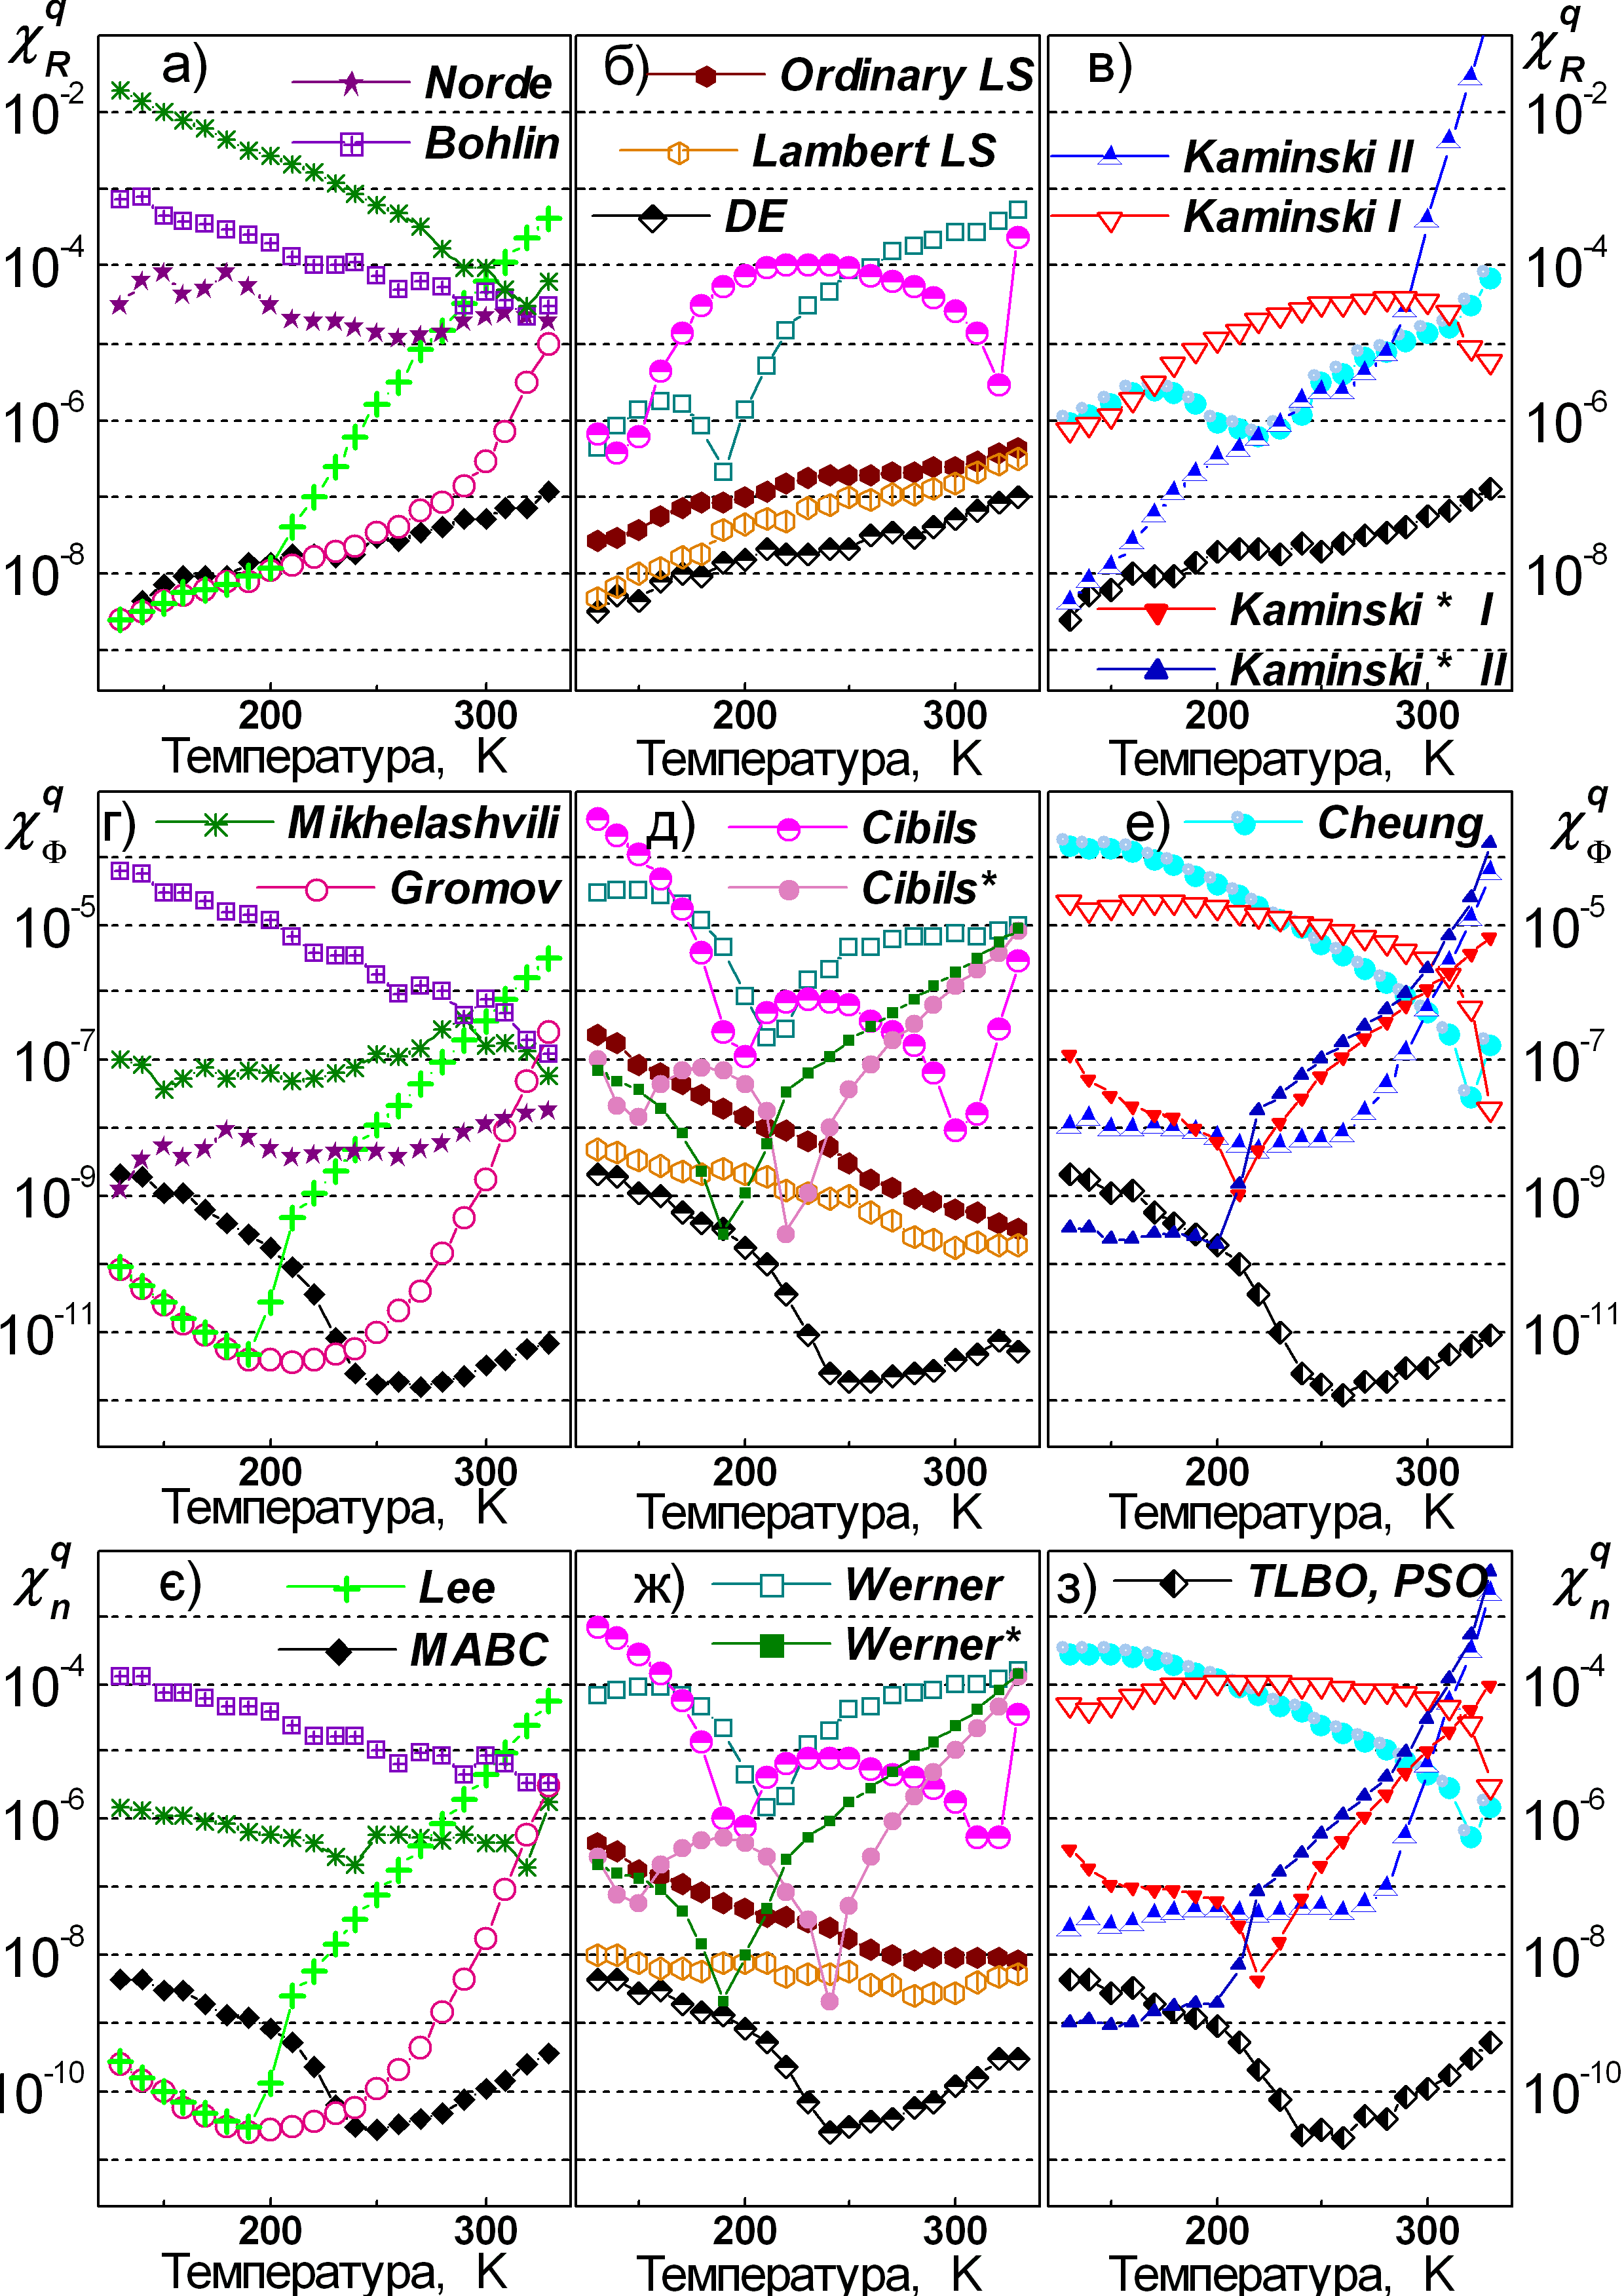
\includegraphics[width=0.85\textwidth]{figId}%
\caption{\label{figId}
Температурні залежності відносних похибок визначення $R_s$ (а --- в), $\Phi_b$ (г --- е) та $n_\mathrm{id}$ (є --- з) при застосуванні різних методів до ідеальних синтезованих ВАХ
%Залежності точності визначення послідовного опору (а --- в), ВБШ (г --- е) та фактора неідеальності (є --- з) при використанні різних методів від температури.
%Результати отримані при використанні ідеальних синтезованих ВАХ.
}
\end{figure}

Точність визначення параметрів з окремої ВАХ залежно від температури, при якій її синтезовано, наведено на рис.~\ref{figId}.
Насамперед зауважимо, що наведені дані показують:
\begin{enumerate}[label=\asbuk*),leftmargin=0em,itemindent=1.5em]
%\begin{enumerate}[label=\asbuk*),labelindent=0em,itemindent=1.5em]
\item при використанні всіх еволюційних алгоритмів для аналізу однакових ВАХ були отримані дуже близькі значення як послідовного опору, так і ВБШ та фактора неідеальності;
це цілком очікуваних результат, пов'язаний з тим що у всіх випадках використовувалася ідентична цільова функція;
\item використання адаптивної процедури в методі Gromov дає можливість суттєво знизити помилки визначення параметрів;
\item використання функції Ламберта при числових обчисленнях дозволяє зменшити помилки визначення параметрів порівняно з випадком, коли в методі найменших квадратів використовується трансцендентна форма рівняння ВАХ;
\item при застосуванні методів Werner, Cibils, та Kaminskii~I шляхом лінійної апроксимації допоміжної функції доцільно визначати лише величину послідовного опору,
тоді як $\Phi_b$ та $n_\mathrm{id}$ краще екстрагувати на наступному етапі, при лінійній апроксимацій ВАХ, скорегованої з врахуванням  отриманого значення $R_s$;
іншими словами використання варіантів цих методів, позначених зірочками дозволяє підвищити точність визначення параметрів;
\item найбільшу точність при аналізі ідеальних синтезованих ВАХ вдається досягти при використанні еволюційних алгоритмів, апроксимації за допомогою методу найменших квадратів з використанням функції Ламберта, Norde (при визначенні $\Phi_b$), Ordinary LS (при визначенні $R_s$), методу Gromov, доповненого адаптивною процедурою, та методу Lee (за винятком випадків високих температур та великих значень $I_s$).
\end{enumerate}




\begin{figure}
\center
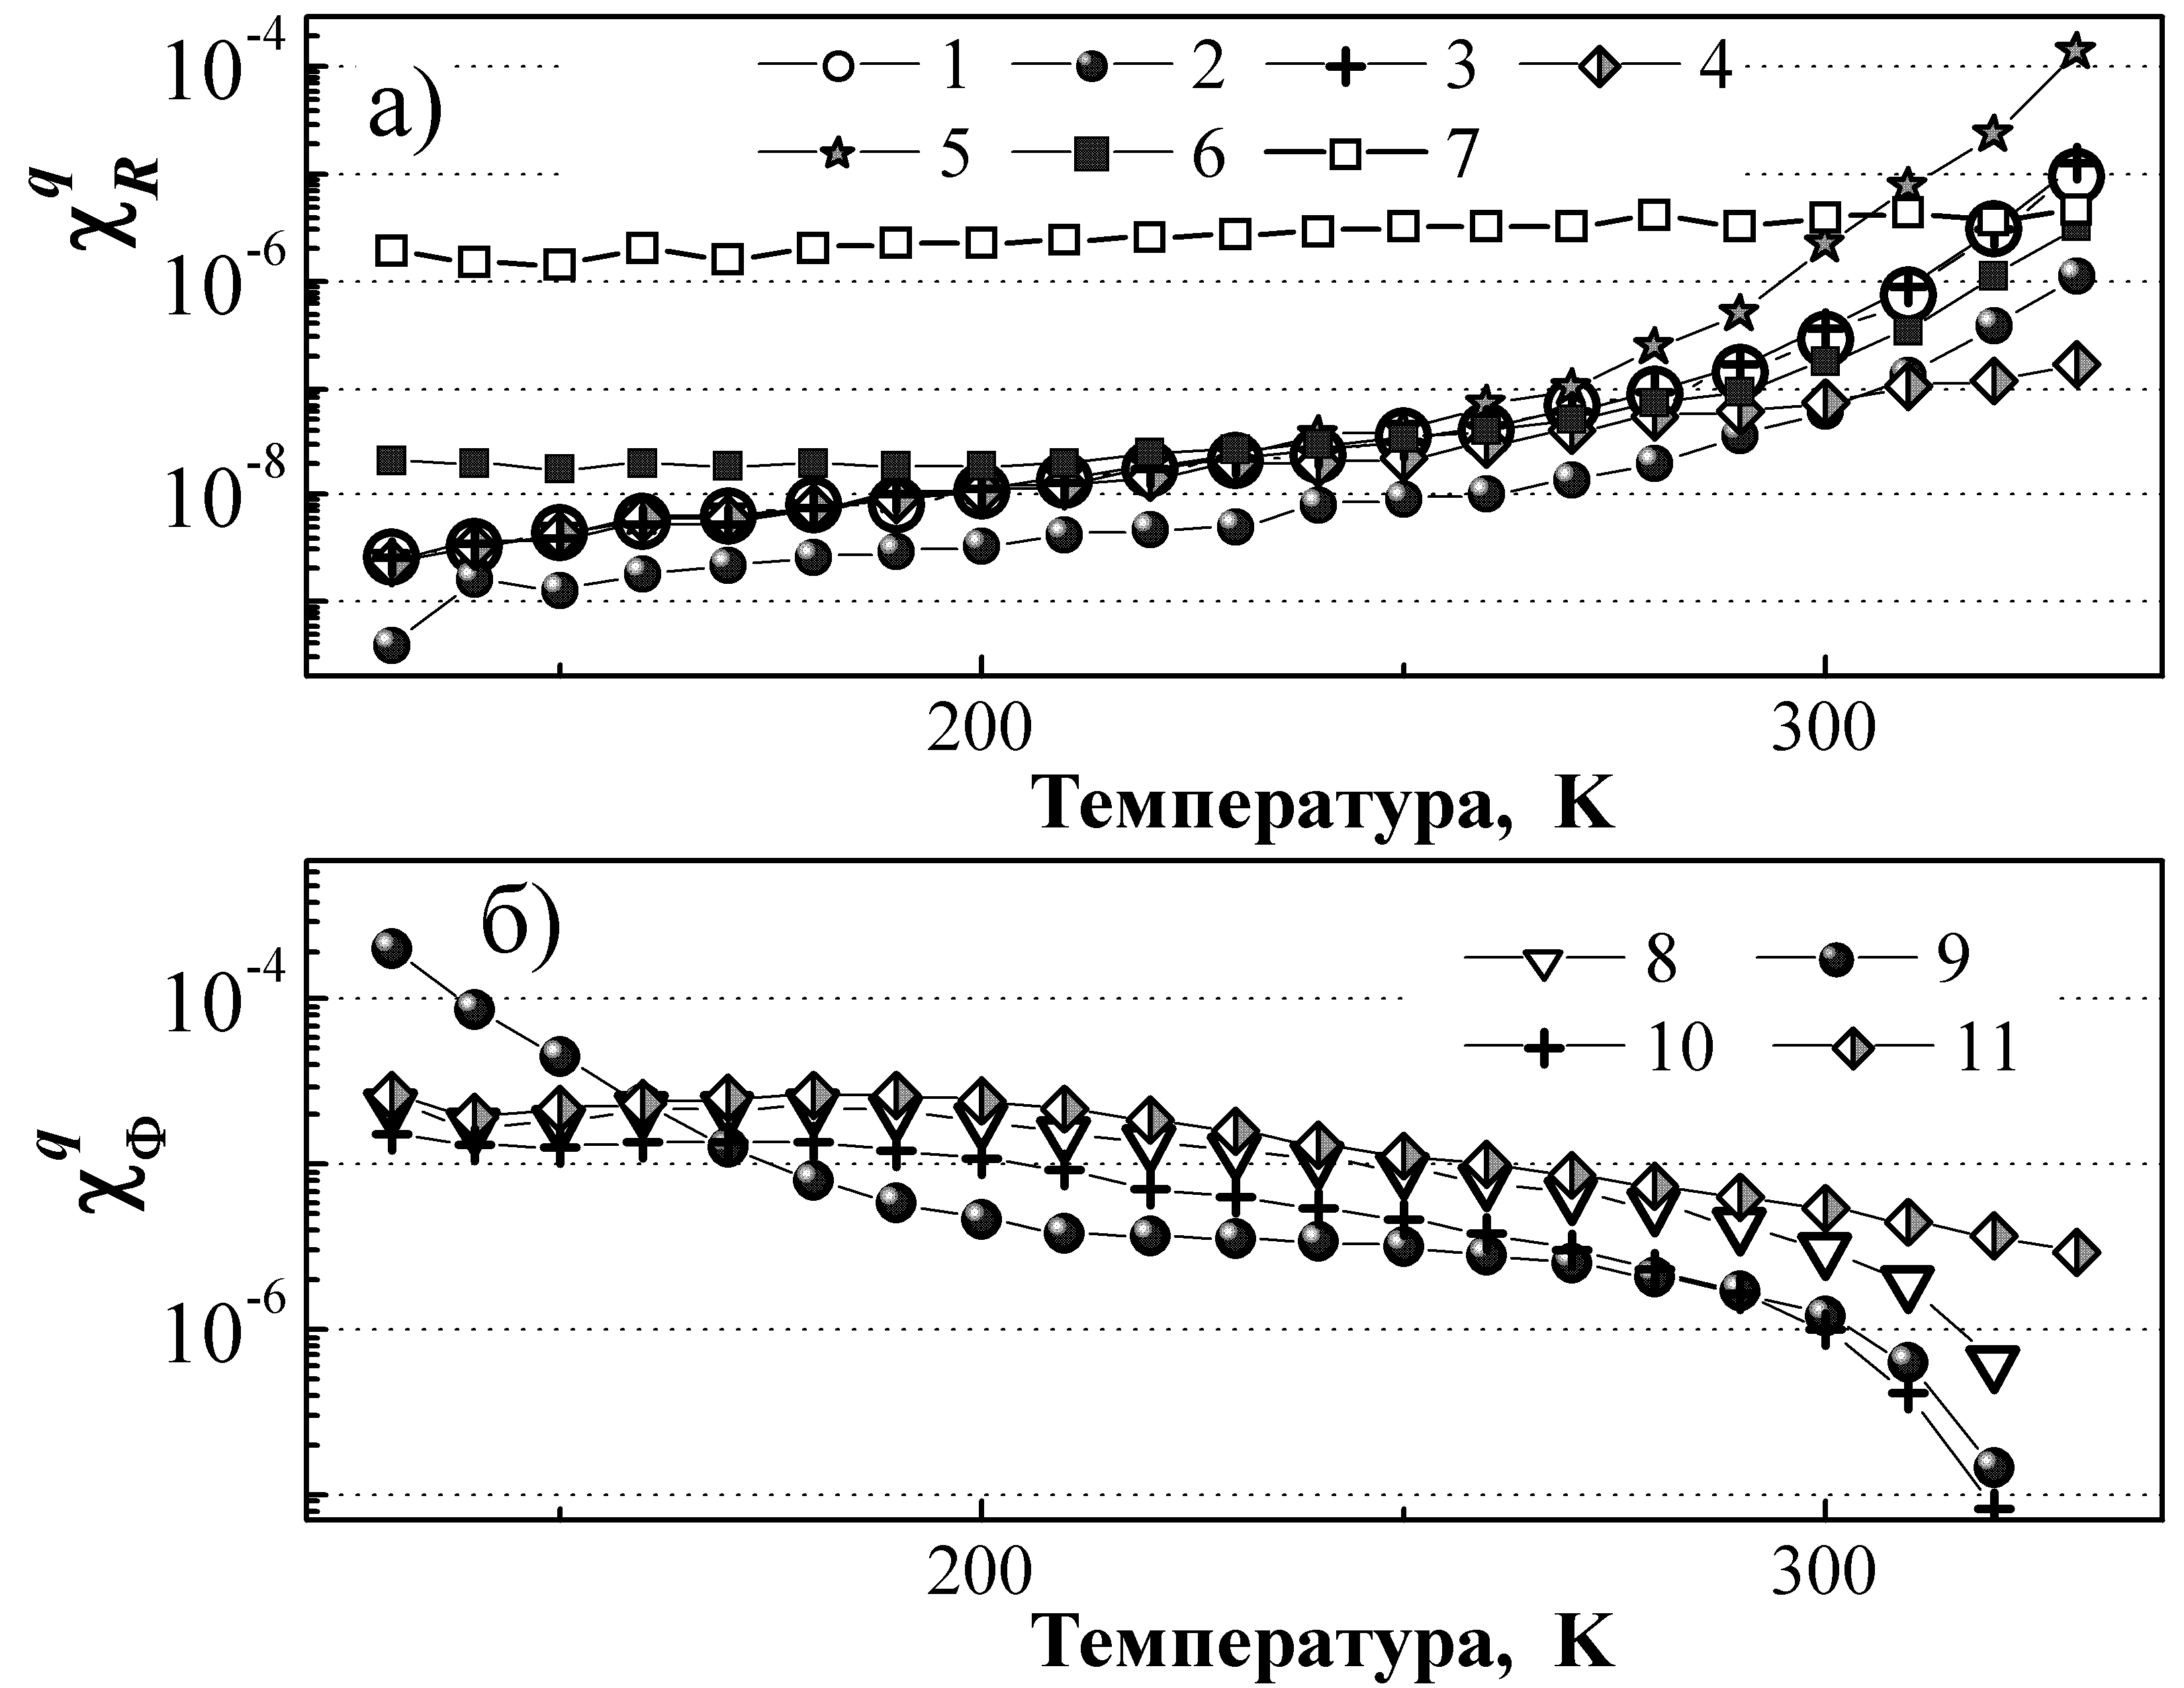
\includegraphics[width=0.65\textwidth]{figCon}%
\caption{\label{figCon}
Температурні залежності похибок визначення $R_s$ (a) та $\Phi_b$ (б) при використанні методів Gromov (a) та  Kaminskii I (б).
Під час синтезу ВАХ використовувалися параметри, величини яких переважно визначались формулами~(\ref{eqSDIs}--\ref{eqRsT}),
проте для  побудови кривих 2 та 9 використовувалися ВАХ для яких значення $R_s$ було в 3 рази більше,
для кривих 3 та 10 величина $n_\mathrm{id}$ була в 1,2 раза більша,
для кривих 4 та 11 величина $I_s$ була в 100 разів менша,
для кривої 5 значення $\Phi_b$ було зменшено на 0,1 еВ,
для кривої 6 величини $R_s$ та $\Phi_b$ залишалися незмінними та рівними 2~Ом та 0,7~еВ, відповідно, під час синтезу всього
набору ВАХ (були незалежні від температури),
для кривої 7 значення $R_s$ та $I_s$ були незмінні та рівні 2~Ом та $10^{-5}$~A, відповідно
}
\end{figure}

З іншого боку, наведені результати показують, що точність визначення параметрів змінюється для різних ВАХ з одного набору (залежить від температури, при якій ВАХ була синтезована).
Фактично мова йде про те, що похибка визначення параметра з масиву $\left\{R_s\,,\,n_\mathrm{id}\,,\, I_s\right\}$ залежить як від його величини, так і від значення інших характеристик ДШ з цього набору.
Для виявлення подібних залежностей всі методи були також застосовані до синтезованих даних, при створенні яких вважалося, що одна з величин з набору ($R_s$, $\Phi_b$, $I_s$ $n_\mathrm{id}$) відрізняється за значенням від того, який очікується згідно з виразами ~(\ref{eqSDIs}--\ref{eqRsT}).
Деякі характерні результати наведені на рис.~\ref{figCon}.

Рис.~\ref{figCon},a показує що, похибки визначення послідовного опору при використанні методу Gromov
\begin{enumerate}[label=\asbuk*),leftmargin=0em,itemindent=1.5em]
\item зростають з підвищенням $\Phi_b$;
\item зменшуються при збільшенні $R_s$ та зменшенні $I_s$;
\item залишаються практично постійними при зміні $n_\mathrm{id}$.
\end{enumerate}
Очевидно, що $I_s$ та $\Phi_b$ пов'язані між собою співвідношенням~(\ref{eqSDIs}).
Проте, на нашу думку, саме величина струму насичення, а не ВБШ, є першочерговим фактором впливу на процес визначення $R_s$.
На користь цього висновку свідчать криві 6 та 7 на рис.~\ref{figCon},a.
Крива 6 була отримана для набору ВАХ, які синтезовані використовуючи припущення що незалежними від температури є як $R_s$, так і $\Phi_b$.
Незважаючи на ці обмеження, $\chi^q_R$ зростає при збільшенні температури.
На противагу, крива 7, отримана для незалежних від температури $R_s$ та $I_s$, показує, що точність визначення послідовного опору залишається практично постійною для всього набору ВАХ.
З іншого боку, рис.~\ref{figCon},б показує, що при використанні методу Kaminskii I зменшення струму насичення підвищує похибку визначення ВБШ.
Загалом проведені дослідження показують, що величина $I_s$ є основним, а величина  $\Phi_b$ другорядним визначальними факторами для точності екстракції інших параметрів (не лише $R_s$) при використанні різних методів (не лише Gromov).
З рис.~\ref{figCon},б також видно, що похибка визначення $\Phi_b$ зменшується у випадку більших значень фактора неідеальності (криві 8 та 10).
В той же час збільшення послідовного опору немонотонно впливає на точність екстракції ВБШ (криві 8 та 9 на рис.~\ref{figCon},б):
при низьких температурах (високих значеннях $\Phi_b$) $\chi^q_{\Phi}$ зростає, при високих $T$ --- навпаки, зменшується.

Узагальнюючи аналіз отриманих результатів, можна зробити висновок, що точність визначення кожного з параметрів зазвичай зростає зі збільшенням його величини.
Проте похибка визначення $\chi^q_{x_i}$ даного параметра ($x_i\in\left\{R_s\,,\,n_\mathrm{id}\,,\, I_s\right\}$) залежить також і від абсолютних величин інших характеристик ДШ ($x_j,\,j\neq i$), причому характер цих залежностей є функцією абсолютних значень кожного параметра з набору і змінюється при використанні різних методів ($\chi^q_{x_i}=f(x_i,\,x_j,\,\text{метод})$).


\begin{figure}
\center
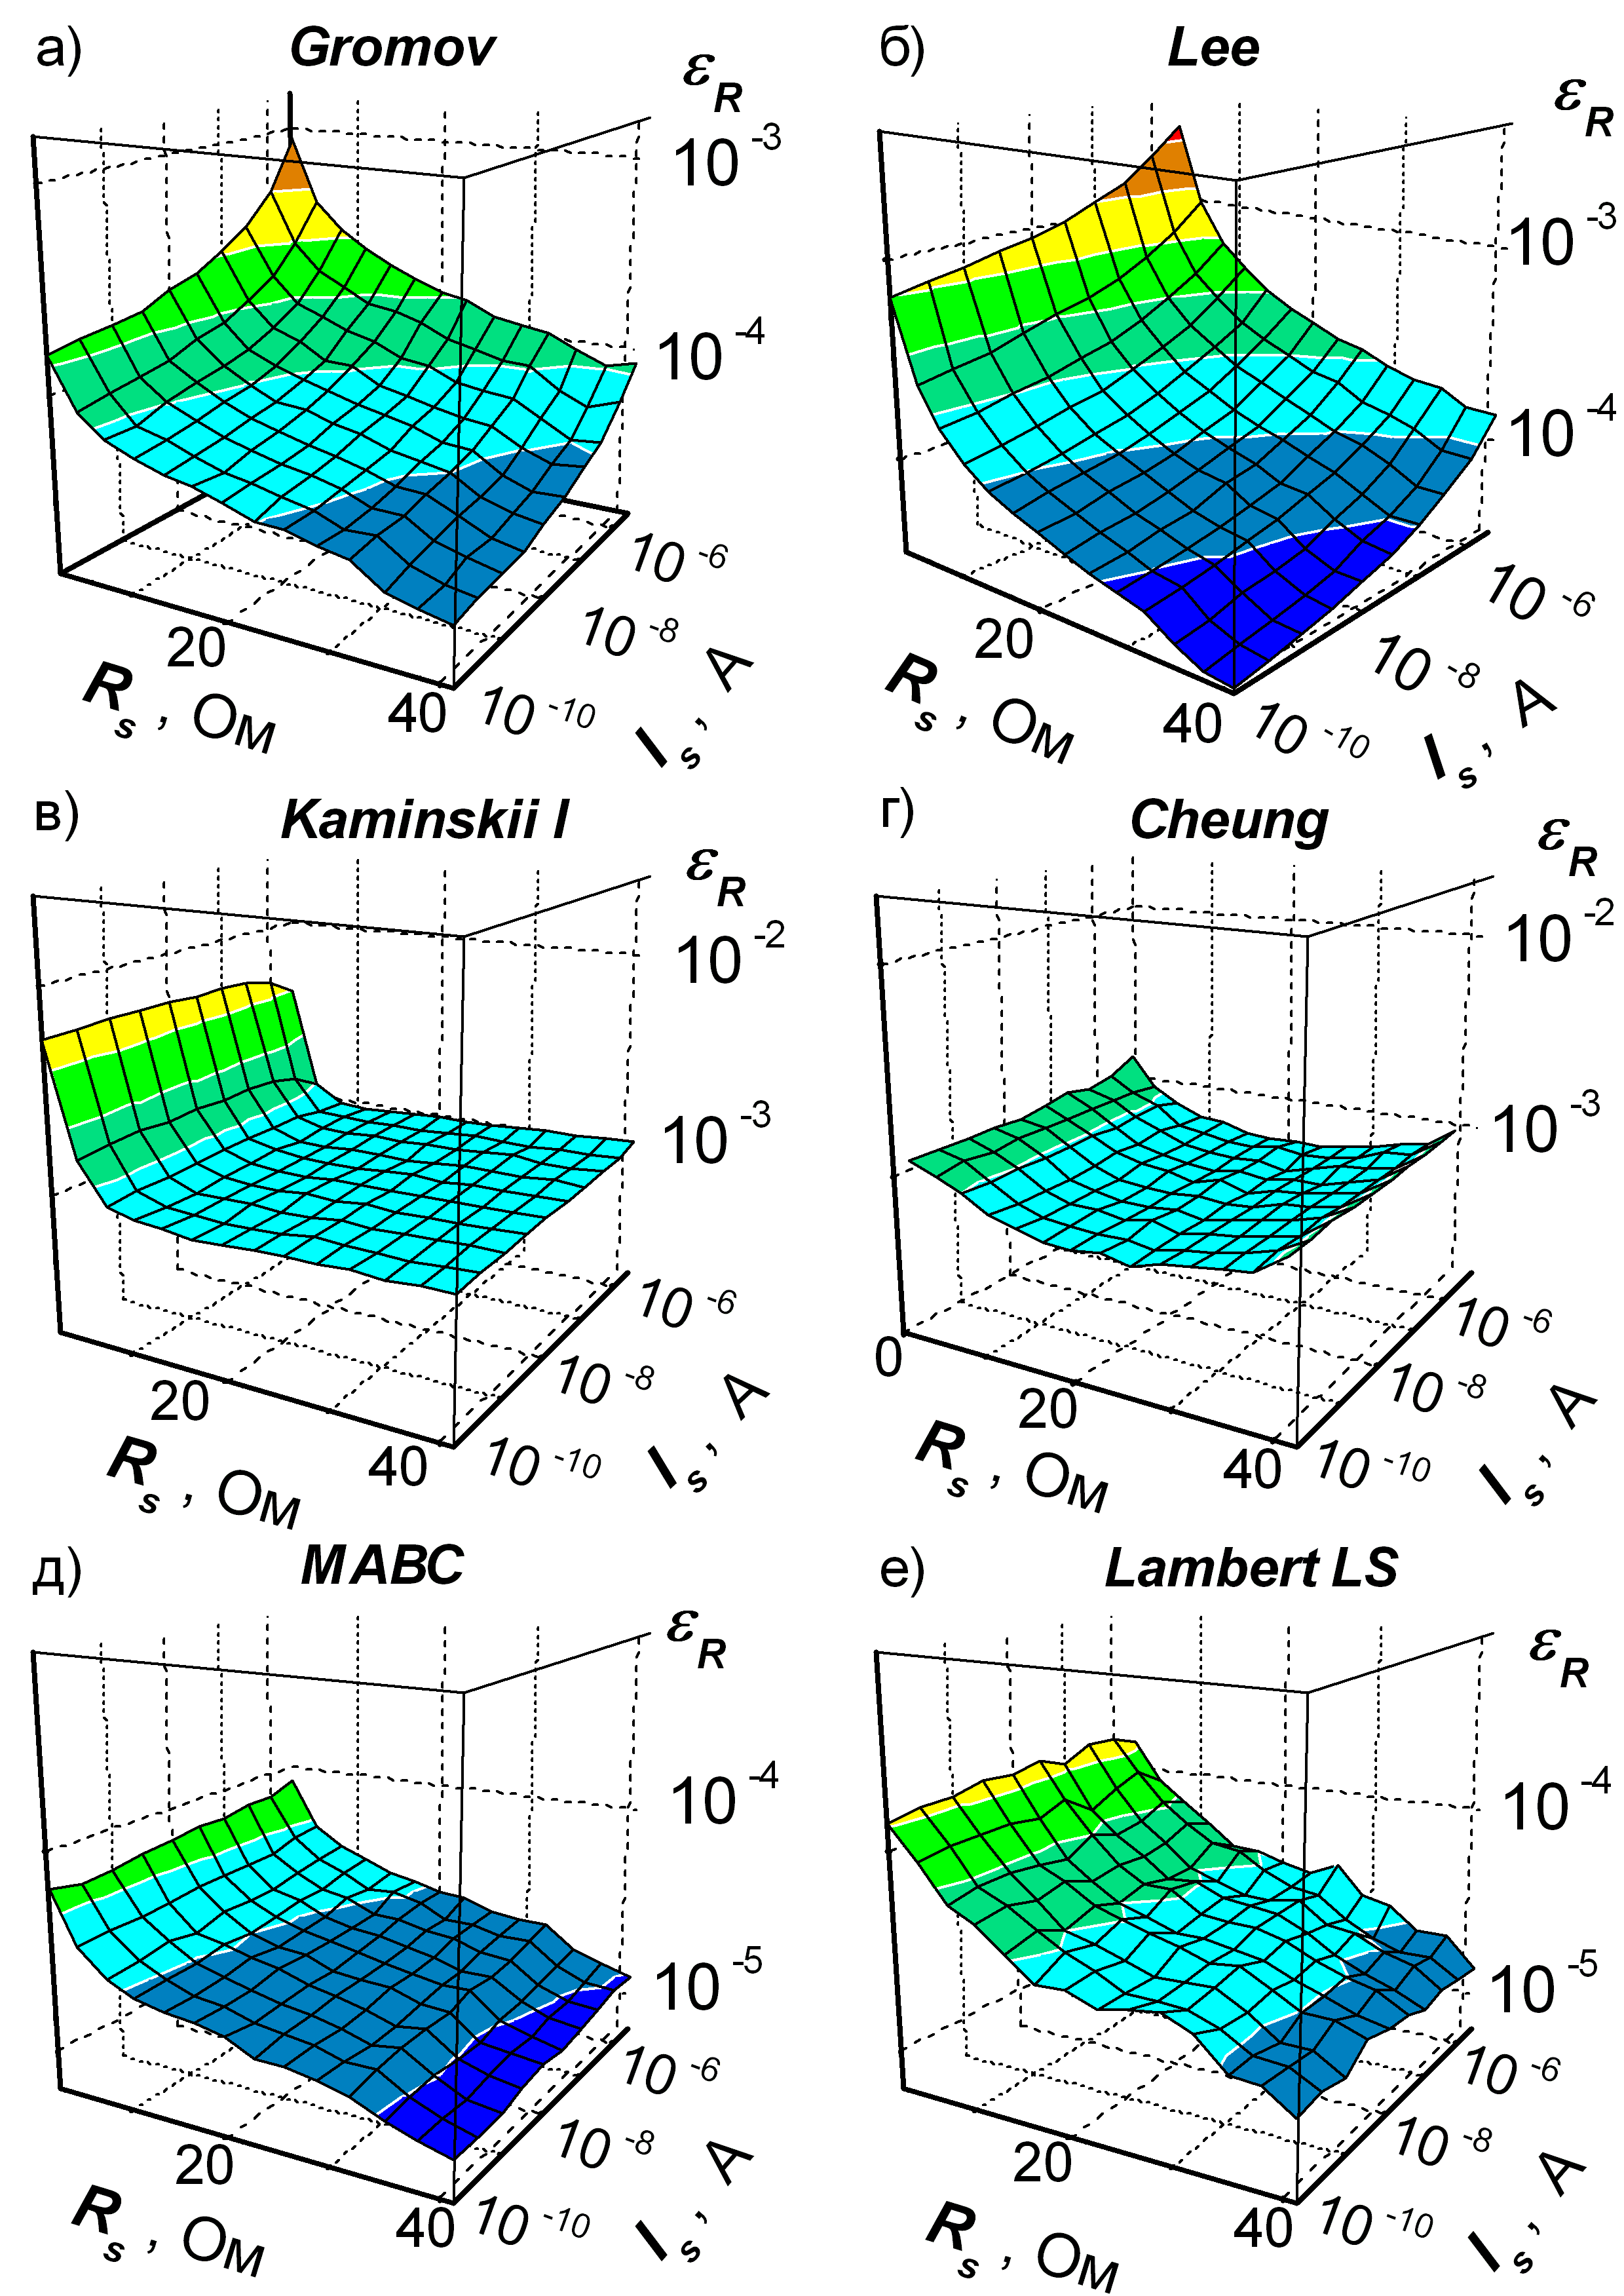
\includegraphics[width=0.8\textwidth]{figR3D}%
\caption{\label{figR3D}
Похибки визначення величини послідовного опору з набору ВАХ, який був синтезований при постійних значеннях $R_s$ та $I_s$.
Показані результати застосування методів Gromov (a), Lee (б), Kaminskii I (в), Cheung (г), MABC (д) та and Lambert LS (е)
}
\end{figure}

\begin{figure}
\center
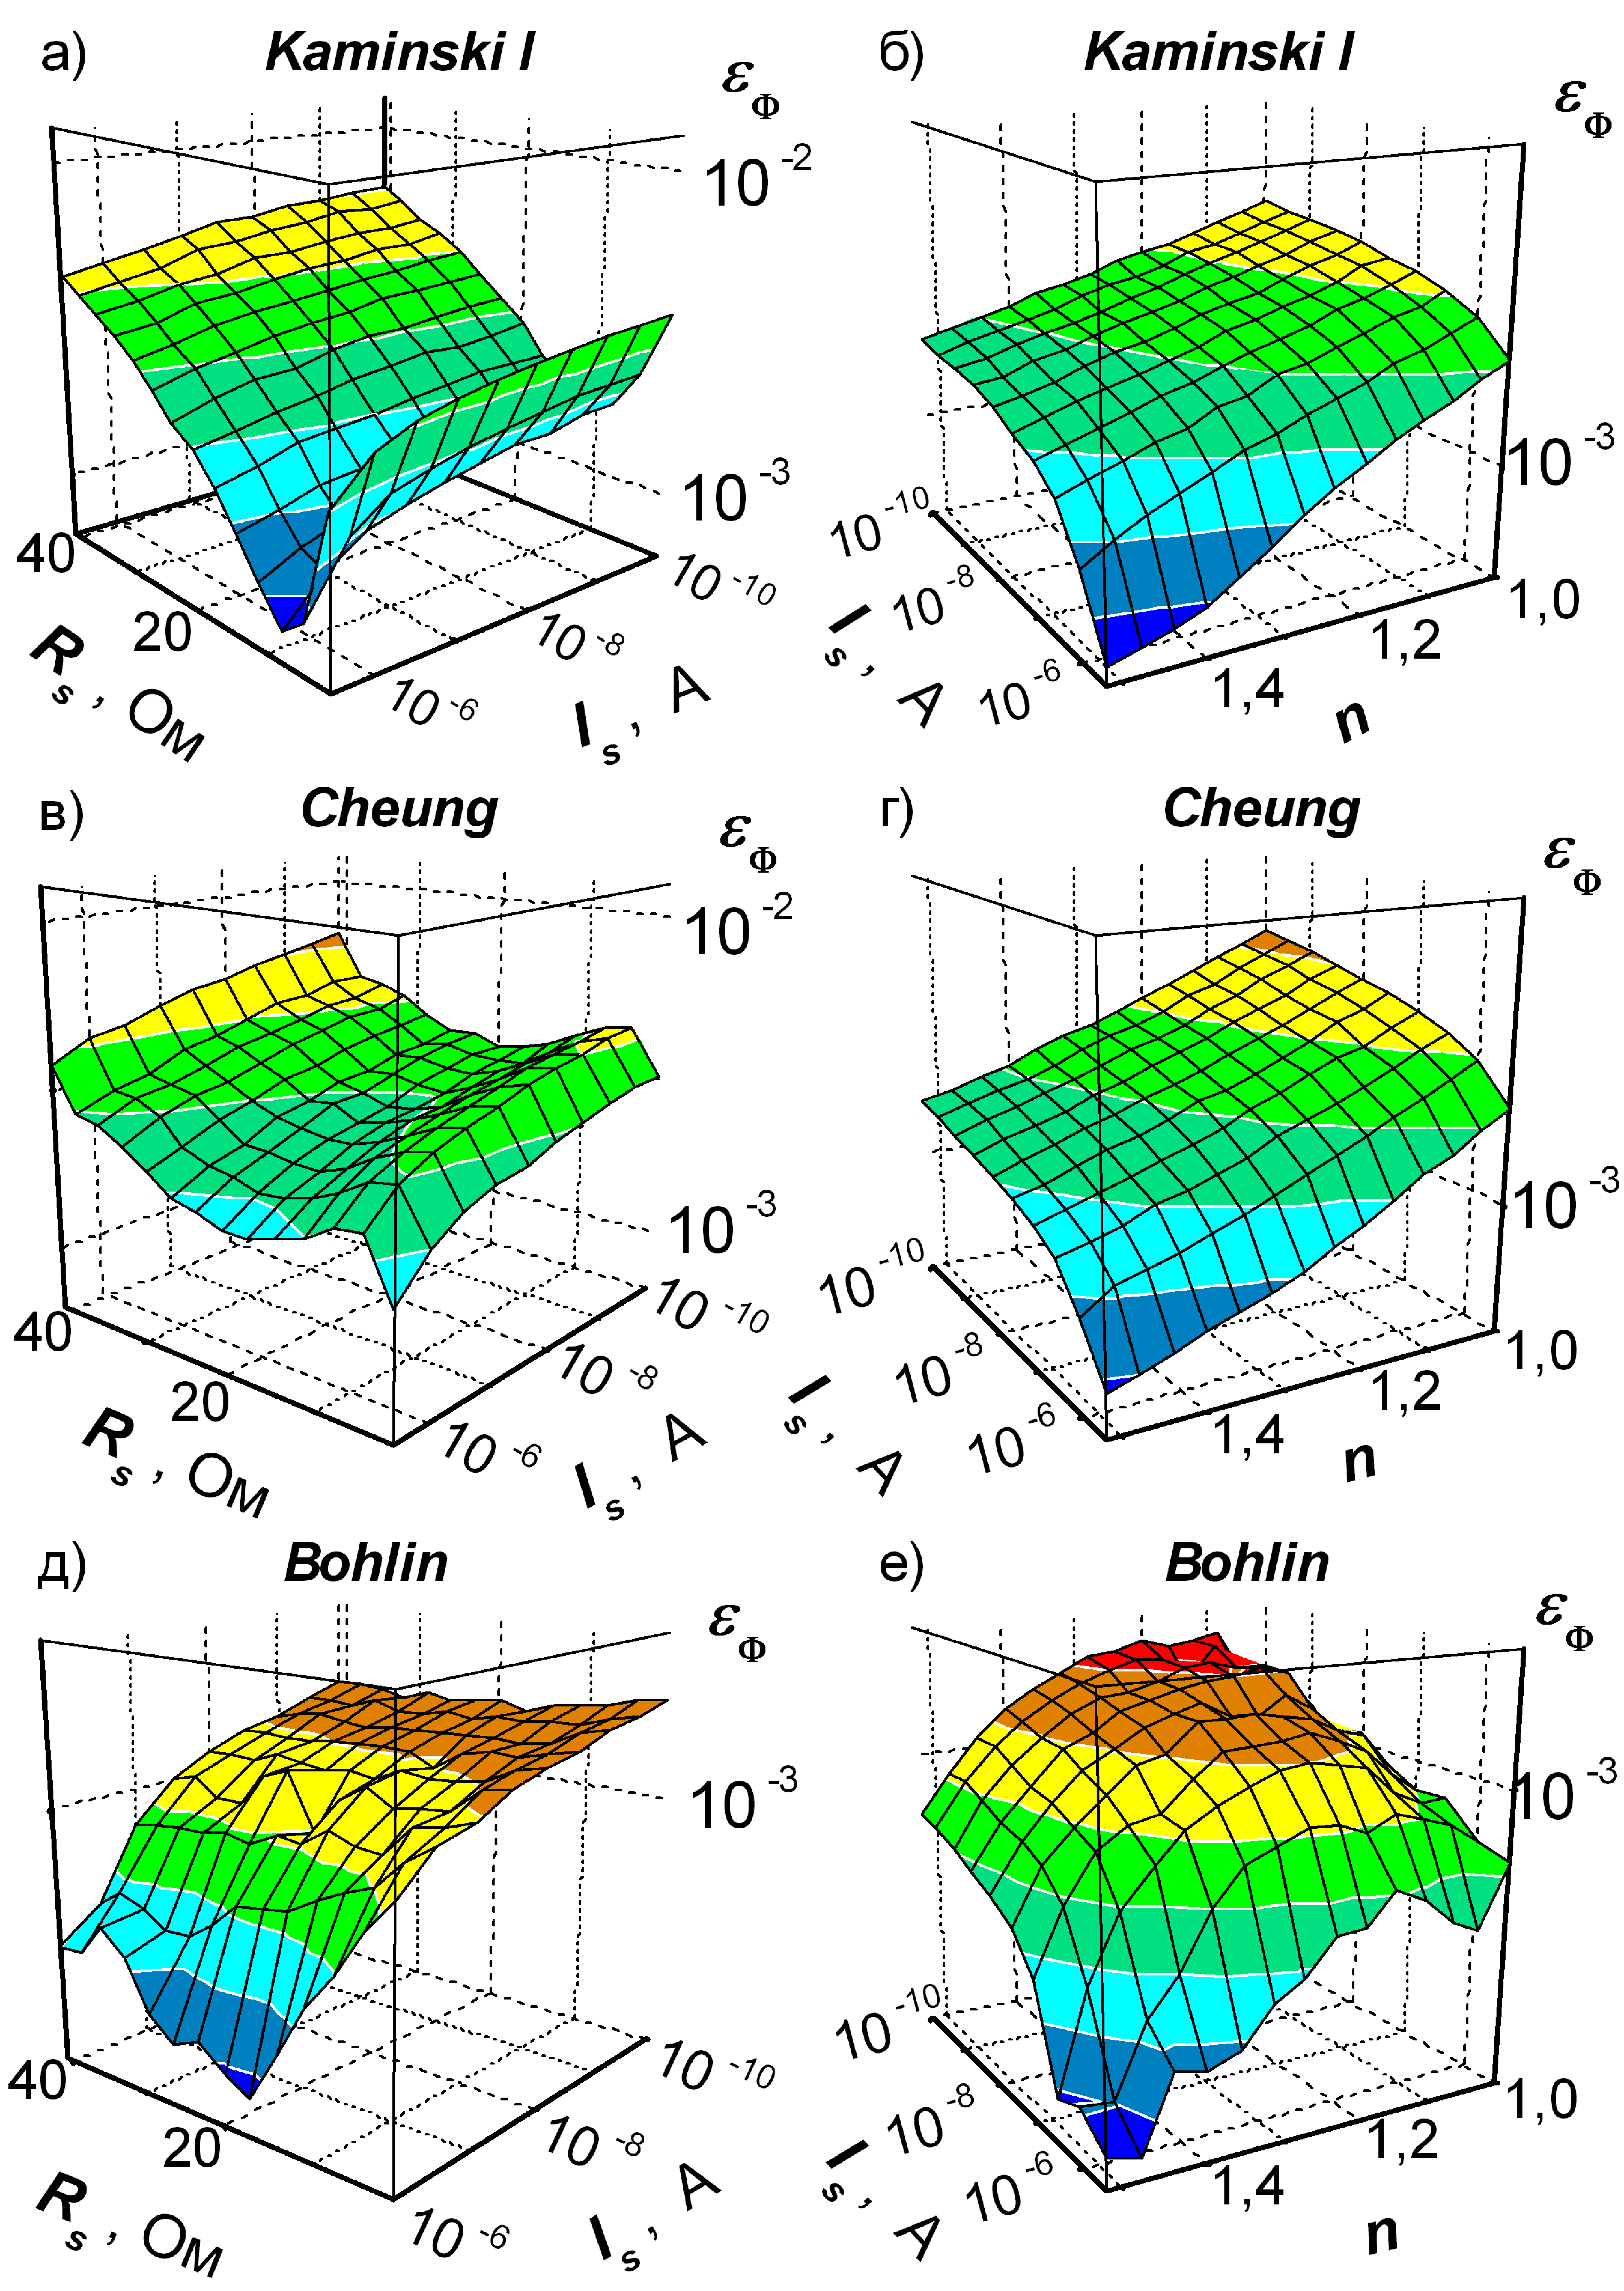
\includegraphics[width=0.8\textwidth]{figF3D}%
\caption{\label{figF3D}
Похибки визначення величини висоти бар'єру Шотткі опору з набору ВАХ, який був синтезований при постійних значеннях $R_s$ та $I_s$ (рисунки а, в та д) або постійних значеннях $n_\mathrm{id}$ та $I_s$ (рисунки б, г, е).
Показані результати застосування методів Kaminskii I (a, б), Cheung (в, г) та Bohlin (д, е)
}
\end{figure}


\begin{figure}
\center
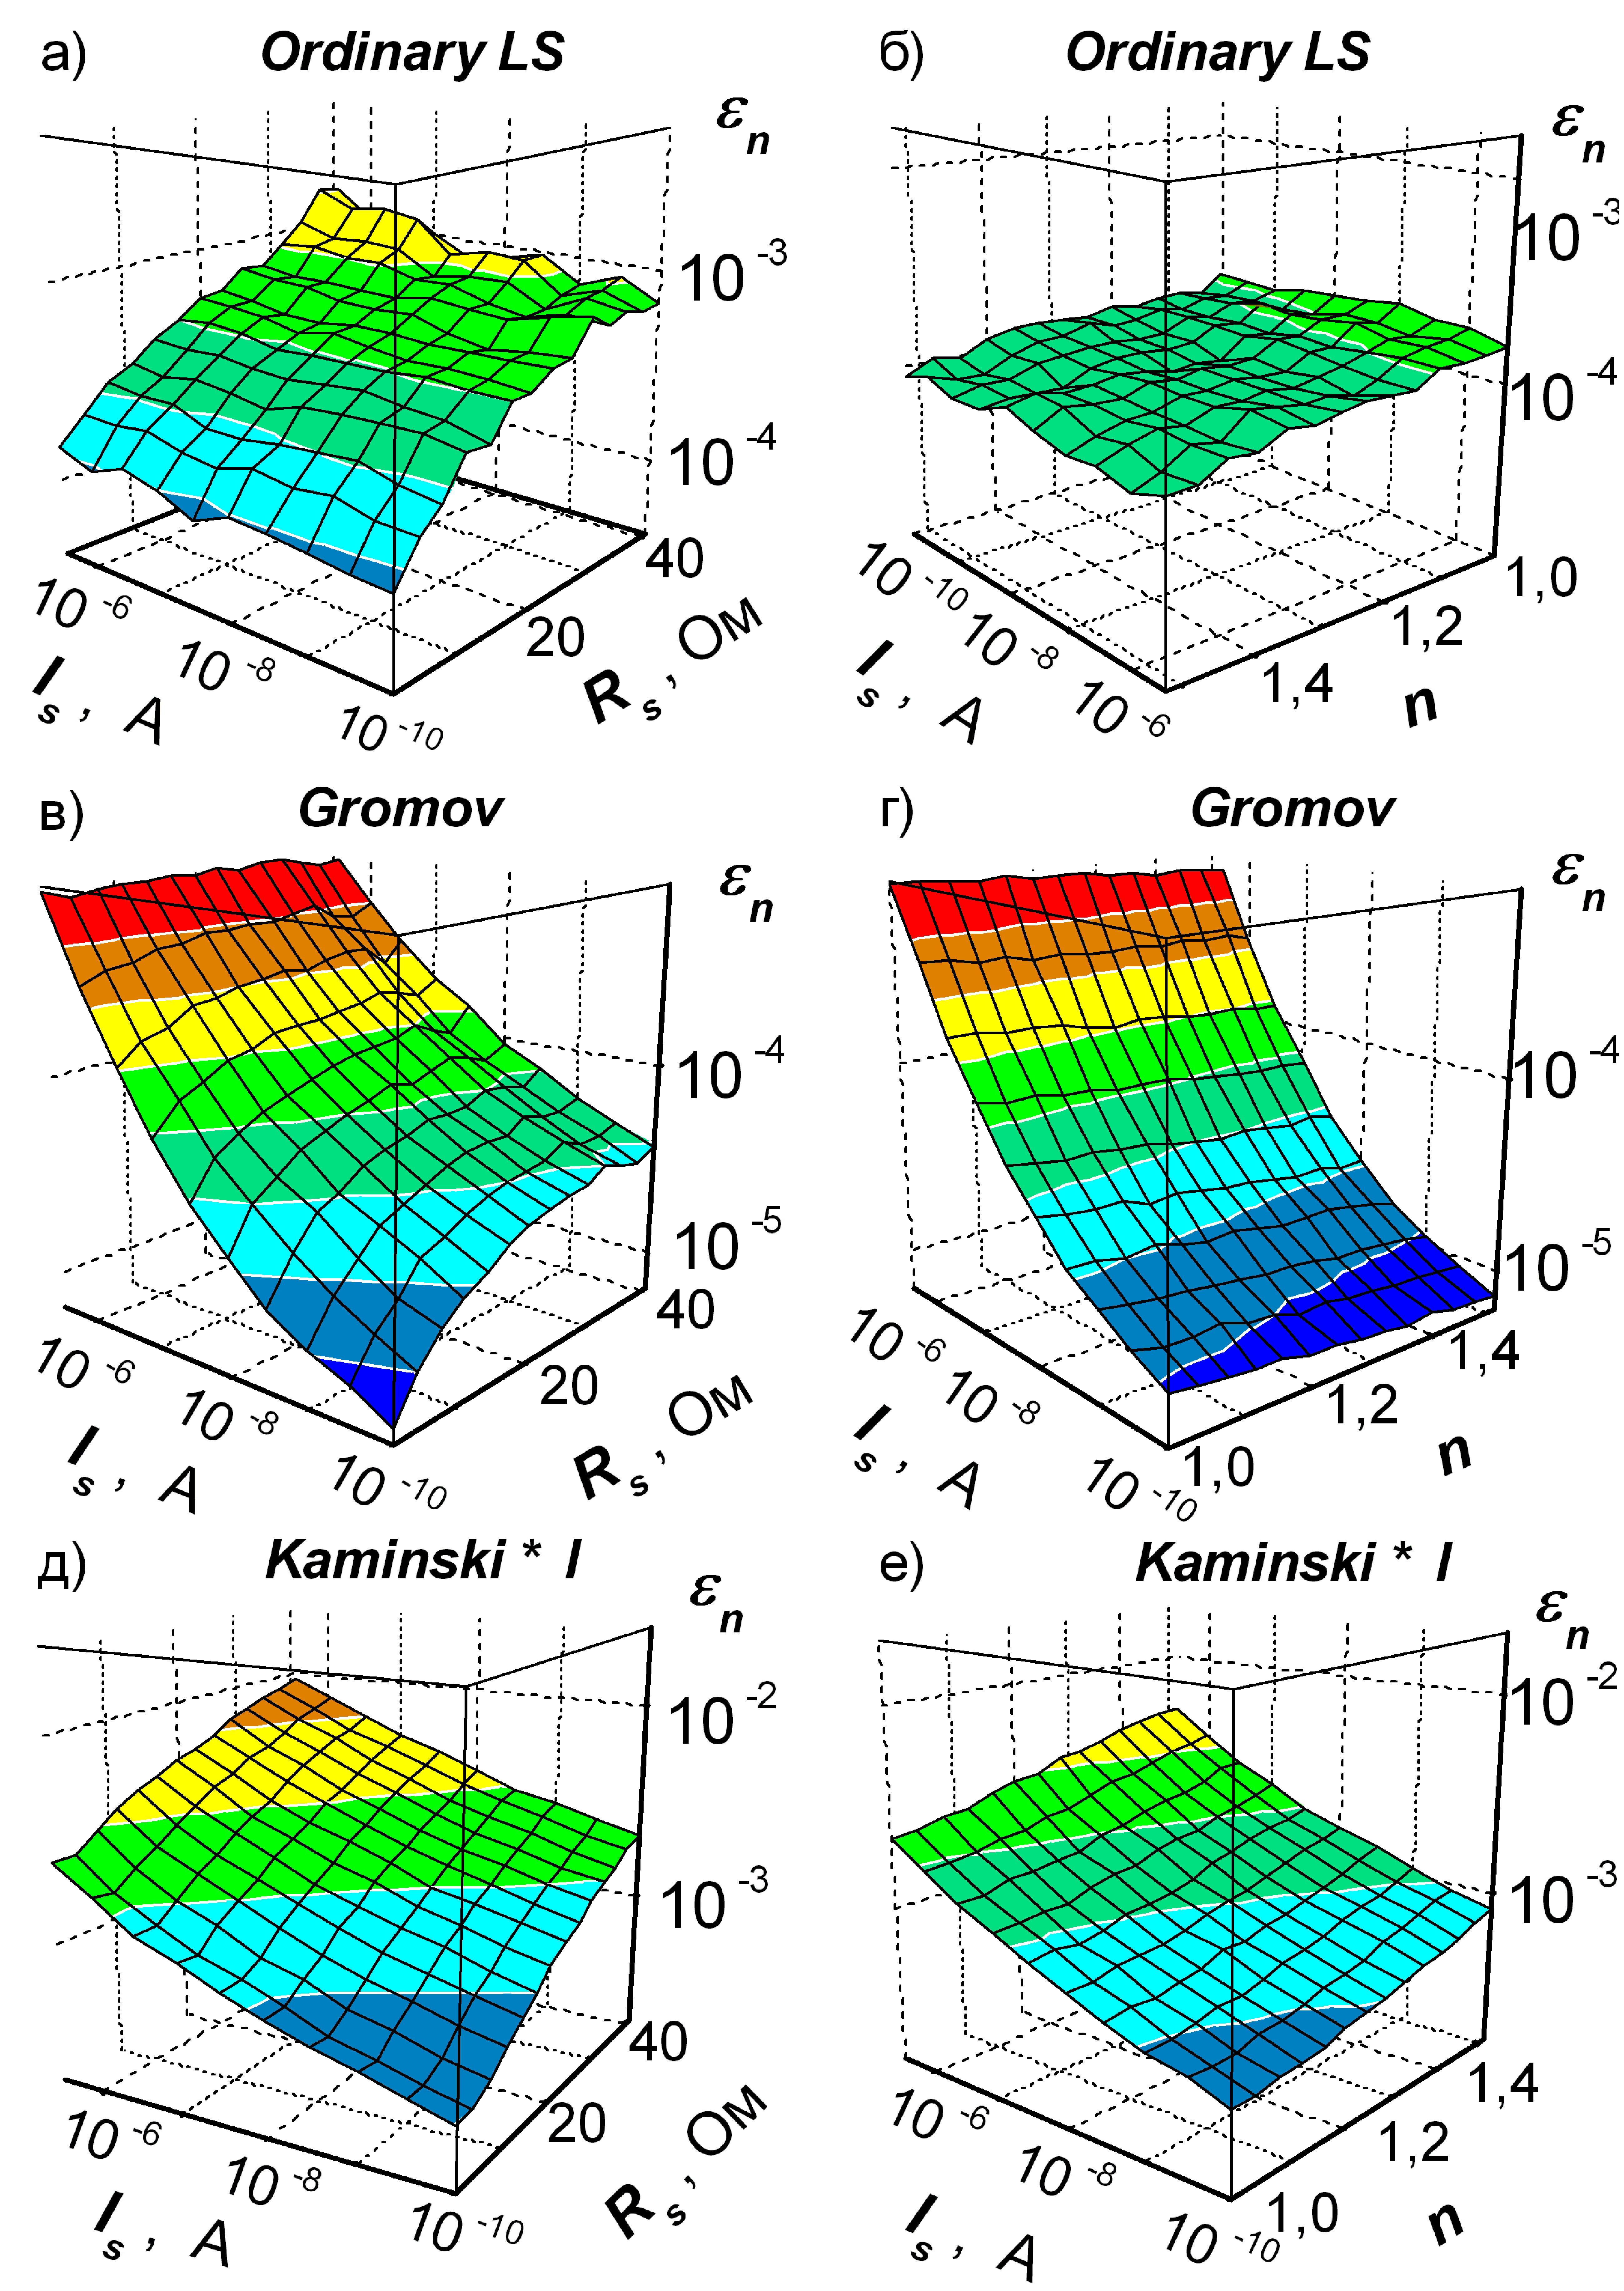
\includegraphics[width=0.8\textwidth]{fign3D}%
\caption{\label{fign3D}
Похибки визначення величини фактора неідеальності з набору ВАХ, який був синтезований при постійних значеннях $R_s$ та $I_s$ (рисунки а, в та д) або постійних значеннях $n_\mathrm{id}$ та $I_s$ (рисунки б, г, е).
Показані результати застосування методів Ordinary LS (a, б), Gromov (в, г) та Kaminskii*~I (д, е)
}
\end{figure}

Для того, щоб виявити основні тенденції цих залежностей були проведені додаткові дослідження.
А саме, були синтезовані набори ВАХ, при побудові яких вважалося, що деякі параметри є незалежними від температури.
В цьому випадку
а)~постійними у всьому температурному діапазоні вважалася два параметри ($R_s$ та $I_s$  або $n_\mathrm{id}$ та $I_s$ для різних наборів ВАХ);
б)~$n_\mathrm{id}$ (або $R_s$) обчислювалися відповідно до того, як описано раніше, в розділі~\ref{SubData}.
Було створено сукупність наборів ВАХ, для яких незалежні від температури величини $R_s$, $n_\mathrm{id}$ та $I_s$ змінювались в діапазонах від
2 до 41~Ом, від 1 до 1,52 та від $10^{-10}$ до $5\cdot10^{-5}$~A, відповідно.
Після цього кожний з методів було застосована до кожного з набору ВАХ, визначено величини параметрів, а також їх похибки.
Найбільш типові результати наведено на рис.~\ref{figR3D}--\ref{fign3D}.
Зокрема, рис.~\ref{figR3D},a підтверджує, що при використанні методу Gromov збільшення $R_s$ та $I_s$ призводить до зменшення та збільшення помилки визначення послідовного опору, відповідно.


Отримані результати щодо факторів впливу узагальнено в табл.~\ref{tabIF}.
В цій таблиці використано ряд символів для опису поведінки похибки визначення параметрів при зміні величини фактора впливу.
А саме.
Якщо помилка визначення монотонно зростає або зменшується зі збільшенням впливаючого фактора, то використовувалися символи <<$\downarrow$>> та <<$\uparrow$>>, відповідно.
Наприклад, саме ці символи характеризують кореляцію точності визначення $R_s$ за допомогою методу Gromov та величини $R_s$ та $I_s$.



\begin{table}
\caption{\label{tabIF}Фактори впливу на похибки визначення параметрів ДШ$^{1)}$
%\footnote{The presence of $R_s$ or $I_s$ or $n$ in the cell indicates the impact on extracted parameter accuracy;
%the subscript and inside bracket symbol deal with extraction error behavior with influencing factor increasing --- see details in the text.}
}
\centering
\small
\begin{tabular}{|l|c|c|c|}
%\begin{tabularx}{\textwidth}{|l|
%                              >{\centering\arraybackslash}X|
 %                             >{\centering\arraybackslash}X|
  %                            >{\centering\arraybackslash}X|}
\hline
\multicolumn{1}{|c|}{Метод}&\multicolumn{3}{c|}{Визначений параметр}\\
\cline{2-4}
%\hline
 &$R_s$&$\Phi_b$&$n$\\
%Метод &$R_s$&$\Phi_b$&$n$\\
%\hline
%\hline
\hhline{|====|}
Norde &$n_\mathrm{id}^w(\vee)$&$I_s(\downarrow)$&---\\
\hline
Werner &$R_s(\vee)$&$R_s(\downarrow)$, $I_s^w(\downarrow)$, $n_\mathrm{id}^w(\downarrow)$&$R_s(\uparrow)$, $n_\mathrm{id}^w(\downarrow)$\\
\hline
Werner* &$R_s(\vee)$&$R_s(\vee)$, $I_s(\uparrow)$, $n_\mathrm{id}(\uparrow)$&$R_s(\vee)$, $I_s(\uparrow)$, $n_\mathrm{id}^w(\uparrow)$\\
\hline
Cibils &$R_s(\vee)$, $n_\mathrm{id}(\uparrow)$&$R_s(\uparrow)$, $n_\mathrm{id}(\vee)$& $R_s(\uparrow)$, $n_\mathrm{id}(\vee)$\\
\hline
Cibils* &$R_s(\vee)$, $n_\mathrm{id}(\uparrow)$&$R_s(\vee)$, $I_s(\uparrow)$, $n_\mathrm{id}(\uparrow)$& $R_s(\vee)$, $I_s(\uparrow)$, $n_\mathrm{id}(\uparrow)$\\
\hline
Kaminskii I&$R_s(\leftharpoonup)$, $n_\mathrm{id}^w(\downarrow)$&$R_s(\vee)$, $I_s(\downarrow)$, $n_\mathrm{id}(\downarrow)$& $R_s(\vee)$, $I_s^w(\downarrow)$, $n_\mathrm{id}(\downarrow)$\\
\hline
Kaminskii* I&$R_s(\leftharpoonup)$, $n_\mathrm{id}^w(\downarrow)$&$R_s(\uparrow)$, $I_s(\uparrow)$, $n_\mathrm{id}(\uparrow)$& $R_s(\uparrow)$, $I_s(\uparrow)$, $n_\mathrm{id}(\uparrow)$\\
\hline
Kaminskii II&$R_s(\downarrow)$, $I_s(\rightharpoonup)$, $n_\mathrm{id}^w(\uparrow)$&$I_s(\rightharpoonup)$, $n_\mathrm{id}^w(\uparrow)$& $I_s(\rightharpoonup)$\\
\hline
Kaminskii* II&$R_s(\downarrow)$, $I_s(\rightharpoonup)$, $n_\mathrm{id}^w(\uparrow)$&$I_s(\uparrow)$, $n_\mathrm{id}(\uparrow)$& $I_s(\uparrow)$, $n_\mathrm{id}(\uparrow)$\\
\hline
Bohlin &$I_s(\rightharpoondown)$&$I_s(\downarrow)$, $n_\mathrm{id}(\wedge)$& $I_s(\rightharpoondown)$, $n_\mathrm{id}(\wedge)$\\
\hline
Lee &$R_s(\downarrow)$, $I_s(\uparrow)$, $n_\mathrm{id}(\uparrow)$&$I_s(\uparrow)$, $n_\mathrm{id}(\uparrow)$& $I_s(\uparrow)$, $n_\mathrm{id}(\uparrow)$\\
\hline
Gromov &$R_s(\downarrow)$, $I_s(\uparrow)$&$R_s(\uparrow)$, $I_s(\uparrow)$, $n_\mathrm{id}^w(\downarrow)$&$R_s(\uparrow)$, $I_s(\uparrow)$, $n_\mathrm{id}^w(\downarrow)$\\
\hline
Cheung &$R_s^w(\vee)$&$R_s(N)$, $I_s(\downarrow)$, $n_\mathrm{id}(\downarrow)$&$R_s^w(N)$, $I_s(\rightharpoondown)$, $n_\mathrm{id}(\downarrow)$\\
\hline
Mikhelashvili &$R_s(\uparrow)$, $I_s(\downarrow)$, $n_\mathrm{id}^w(\downarrow)$&$R_s(\uparrow)$, $I_s(\wedge)$, $n_\mathrm{id}^w(\downarrow)$&$R_s(\uparrow)$, $I_s(\wedge)$, $n_\mathrm{id}^w(\downarrow)$\\
\hline
Ordinary LS &$R_s(\downarrow)$&$R_s(\uparrow)$, $I_s^w(\downarrow)$, $n_\mathrm{id}^w(\downarrow)$&$R_s(\uparrow)$, $n_\mathrm{id}^w(\downarrow)$\\
\hline
Lambert LS &$R_s(\downarrow)$&$I_s^w(\downarrow)$&$n_\mathrm{id}^w(\downarrow)$\\
\hline
EAs &$R_s(\downarrow)$, $I_s^w(\uparrow)$&$R_s(\uparrow)$, $I_s(\vee)$, $n_\mathrm{id}^w(\downarrow)$&$R_s(\uparrow)$, $I_s(\vee)$, $n_\mathrm{id}^w(\downarrow)$\\
\hline
\multicolumn{4}{|p{0.9\textwidth}|}{$^{1}$\textit{Наявність $R_s$ або $I_s$ або $n_\mathrm{id}$ в клітинці означає
вплив величини, відповідно, послідовного опору або струму насичення або фактора неідеальності на точність визначення параметра;
верхній індекс та символ в дужках пов'язані з характером поведінки точності визначення параметра при збільшенні $R_s$ або $I_s$ або $n_\mathrm{id}$ --- деталі див. у тексті.
}}\\
\hline
\end{tabular}
%\end{tabularx}
\end{table}

Виявлено, може залежати від фактора впливу не лише монотонно.
Наприклад, рис.~\ref{figCon},б та рис.~\ref{figF3D},a показують, що при використанні методу Kaminskii~I похибка визначення $\Phi_b$ зростає з підвищенням послідовного опору при великих ($>10$~Ом) значеннях $R_s$ і зменшується при малих величинах $R_s$.
Для позначення залежності з такою поведінкою в табл.~\ref{tabIF} використовується символ <<$\vee$>>.
Подібна залежність спостерігається при використанні метода Chueng для визначення $R_s$ (рис.~\ref{figR3D},г).
Проте в цьому випадку сама величина $R_s$ порівняно слабко впливає на точність визначення послідовного опору.
Схожі слабкі залежності позначаються в табл.~\ref{tabIF} за допомогою верхнього індексу  <<$w$>>.
Інші приклади слабких залежностей $I_s$ та  $n_\mathrm{id}$ можна побачити на рис.~\ref{figR3D},д та рис.~\ref{fign3D},г, відповідно.

Якщо графік залежності похибки визначення параметра від величини фактора впливу має не мінімум, а максимум (див., наприклад, рис.~\ref{figF3D},е),
то використовувався символ <<$\wedge$>>.
Наявність на залежності екстремумів обох типів (див., наприклад, рис.~\ref{figF3D},в) позначено за допомогою символу <<$N$>>.

Ще один тип залежності показаний на рис.~\ref{figR3D},в.
При використанні методу Kaminskii~I для визначення  $R_s$ помилки залишаються постійними в широкому діапазоні змін $R_s$ та $I_s$ і зростають лише для малих значень $R_s$.
Подібні залежності між помилкою визначення та впливаючим фактором позначені символом <<$\leftharpoonup$>>.
Символи <<$\rightharpoonup$>> або <<$\rightharpoondown$>> якщо помилки зростають або зменшуються, відповідно, лише при великих значеннях фактора впливу.

З наведених даних, зокрема, видно, що фактори, які впливають на точність екстракції $\Phi_b$ та  $n_\mathrm{id}$ подібні для більшості методів, які розглядалися в роботі.
Використання адаптивної процедури в методі Gromov призводить до того, що точність визначення $\Phi_b$ та  $n_\mathrm{id}$ стає залежною від величини $R_s$, тоді як вплив величини фактора неідеальності послаблюється.
Точність методів Werner*, Cibils* та Kaminskii* більш чутлива до величин параметрів ніж при використанні варіантів цих же методів без зірочок.
Найбільш стійкими до величин параметрів є точності числових методів, особливо при використанні функції Ламберта (Lambert LS).


\subsection{Швидкодія методів визначення параметрів діодів Шотткі}
Ще одним, поряд з точністю, критерієм для характеризації різних методів визначення параметрів структур МН є час, необхідний для визначення параметрів (RT, running time).
Для оцінки RT були використані WinAPI функції $QueryPerformanceCounter()$ та $QueryPerformanceFrequency()$.
Розрахунки проводились на персональному комп'ютері з наступними характеристиками:
\begin{itemize}
  \item процесор AMD A4-3400 2.7~GHz;
  \item 3072~MB RAM;
  \item операційна система Windows XP.
\end{itemize}
Очевидно, що точний час екстракції параметрів залежить від програмної реалізації, від завантаження процесору в даний момент часу тощо.
Тим не менш, всі методи тестувалися за однакових умов, а отже вибраний підхід дозволяє порівняти тривалість роботи різних методів, а також оцінити порядок величини RT.

\begin{table}
\caption{\label{tabRT}Час визначення параметрів ДШ з однієї ВАХ}
\begin{tabularx}{\textwidth}{|>{\raggedright\arraybackslash}X|
                             >{\centering\arraybackslash}X|
                            >{\centering\arraybackslash}X|}
\hline
\multicolumn{1}{|c|}{Метод}&\multicolumn{2}{c|}{Час роботи, с}\\
\cline{2-3}
%\begin{tabular}{lcc}
%Method &\multicolumn{2}{c}{Running time, s}\\
 &максимальний&мінімальний\\
\hhline{|===|}
Norde &$3,7\cdot10^{-5}$&$2,6\cdot10^{-5}$\\ \hline
Werner $^{1)}$ &$4,5\cdot10^{-5}$&$4,0\cdot10^{-5}$\\ \hline
Cibils $^{1)}$ &$5,3\cdot10^{-3}$&$1,9\cdot10^{-4}$\\ \hline
Kaminskii I $^{1)}$ &$8,0\cdot10^{-5}$&$4,5\cdot10^{-5}$\\ \hline
Kaminskii II $^{1)}$ &$2,6\cdot10^{-3}$&$3,0\cdot10^{-4}$\\ \hline
Bohlin &$6,3\cdot10^{-5}$&$4,0\cdot10^{-5}$\\ \hline
Lee &$3,6\cdot10^{-3}$&$1,8\cdot10^{-4}$\\ \hline
Gromov &$2,2\cdot10^{-2}$&$2,2\cdot10^{-2}$\\ \hline
Gromov $^{2)}$ &$4,6\cdot10^{-5}$&$2,7\cdot10^{-5}$\\ \hline
Cheung &$3,2\cdot10^{-5}$&$2,0\cdot10^{-5}$\\ \hline
Mikhelashvili &$4,7\cdot10^{-5}$&$2,9\cdot10^{-5}$\\ \hline
Ordinary LS &$460$&$1,8$\\ \hline
Lambert LS &$540$&$7,6$\\ \hline
DE &$0,73$&$0,36$\\ \hline
PSO &$0,35$&$0,14$\\ \hline
MABC &$0,20$&$5,7\cdot10^{-2}$\\ \hline
TLBO &$19,2$&$5,4$ \\
\hline
\multicolumn{3}{|p{17cm}|}{$^{1}$\textit{Час корекції ВАХ та лінійної апроксимації дорівнює $1.8\cdot10^{-5}$~с (максимальний) або $1.4\cdot10^{-5}$~с (мінімальний)}.
}\\
\multicolumn{3}{|p{17cm}|}{$^{2}$\textit{Для випадку, коли адаптивна процедура не використовується}.
}\\ \hline
\end{tabularx}
\end{table}

Отримані значення RT при застосуванні різноманітних методів до аналізу ідеальних синтезованих ВАХ наведено в табл.~\ref{tabRT}.
Загалом RT залежить від кількості точок у вихідній залежності;
в таблиці наведено значення, отримані при застосування методів до ВАХ, сгенерованих для температур 130~K та 330~K.
Очевидно, що
\begin{enumerate}[label=\asbuk*),leftmargin=0em,itemindent=1.5em]
\item час роботи аналітичних методів при використанні сучасних комп'ютерів знехтувано малий;
\item у випадку ВАХ з великою кількістю експериментальних точок RT числових методів може досягати значних величин;
\item використання функції Ламберта призводить до збільшення часу роботи числових методів; однією з причин цього є необхідність використовувати числовий ряд для обчислення значення самої функції;
\item використання адаптивної функції очікувано викликає збільшення RT на декілька порядків, проте його абсолютне значення залишається невеликим;
\item серед еволюційних алгоритмів найбільш швидким при визначенні параметрів ДШ є MABC, тоді як найбільш повільним --- TLBO.
\end{enumerate}


Узагальнюючи результати, отримані при дослідженні застосування методів до ідеальних синтезованих ВАХ, зауважимо,
що еволюційні алгоритми видаються найбільш придатними для визначення параметрів ДШ завдяки низькому рівню помилок, помірній чутливості точності до величини параметрів
та допустимому часу роботи.
Поряд з цим, іншими методами, яким також варто надавати перевагу є аналітичний метод Gromov з використанням адаптивної процедури та числовий метод Lambert LS.
Проте точність визначення параметрів для першого з них суттєво зменшується при високих значеннях струму насичення (високих температурах).
Щодо методу Lambert LS, то його основним недоліком є значний час, потрібний для обчислень.


\subsection{Вплив випадкових похибок на точність визначення параметрів структур метал--напівпровідник}

На рис.~\ref{figG1003} та рис.~\ref{figDiag} наведено результати застосування різноманітних методів до зашумлених даних.
Цілком очікувано, помилки при екстракції параметрів збільшуються при підвищенні рівня шуму (рівня випадкових помилок вимірювань).
Проте залежності правильності визначення параметрів з однієї ВАХ схожі до отриманих при аналізі ідеальних синтезованих ВАХ.
Як наслідок, фактори впливу на точність також ідентичні, тобто дані табл.~\ref{tabIF} цілком застосовні і в цьому випадку.
Крім того, інші характерні особливості методів, виявлені раніше, проявляються і в цьому випадку.
Наприклад, використання функції Ламберта дозволяє досягнути більшої точності числових методів при визначенні параметрів ДШ.
Еволюційні алгоритми, методи Gromov та Lee характеризуються найменшими помилками.
З іншого боку, різниця між результатами, отриманими за допомогою методів Gromov та Lee зменшується.
Це свідчить про зниження переваги застосування запропонованої адаптивної процедури з підвищенням рівня випадкових похибок.



\begin{figure}
\center
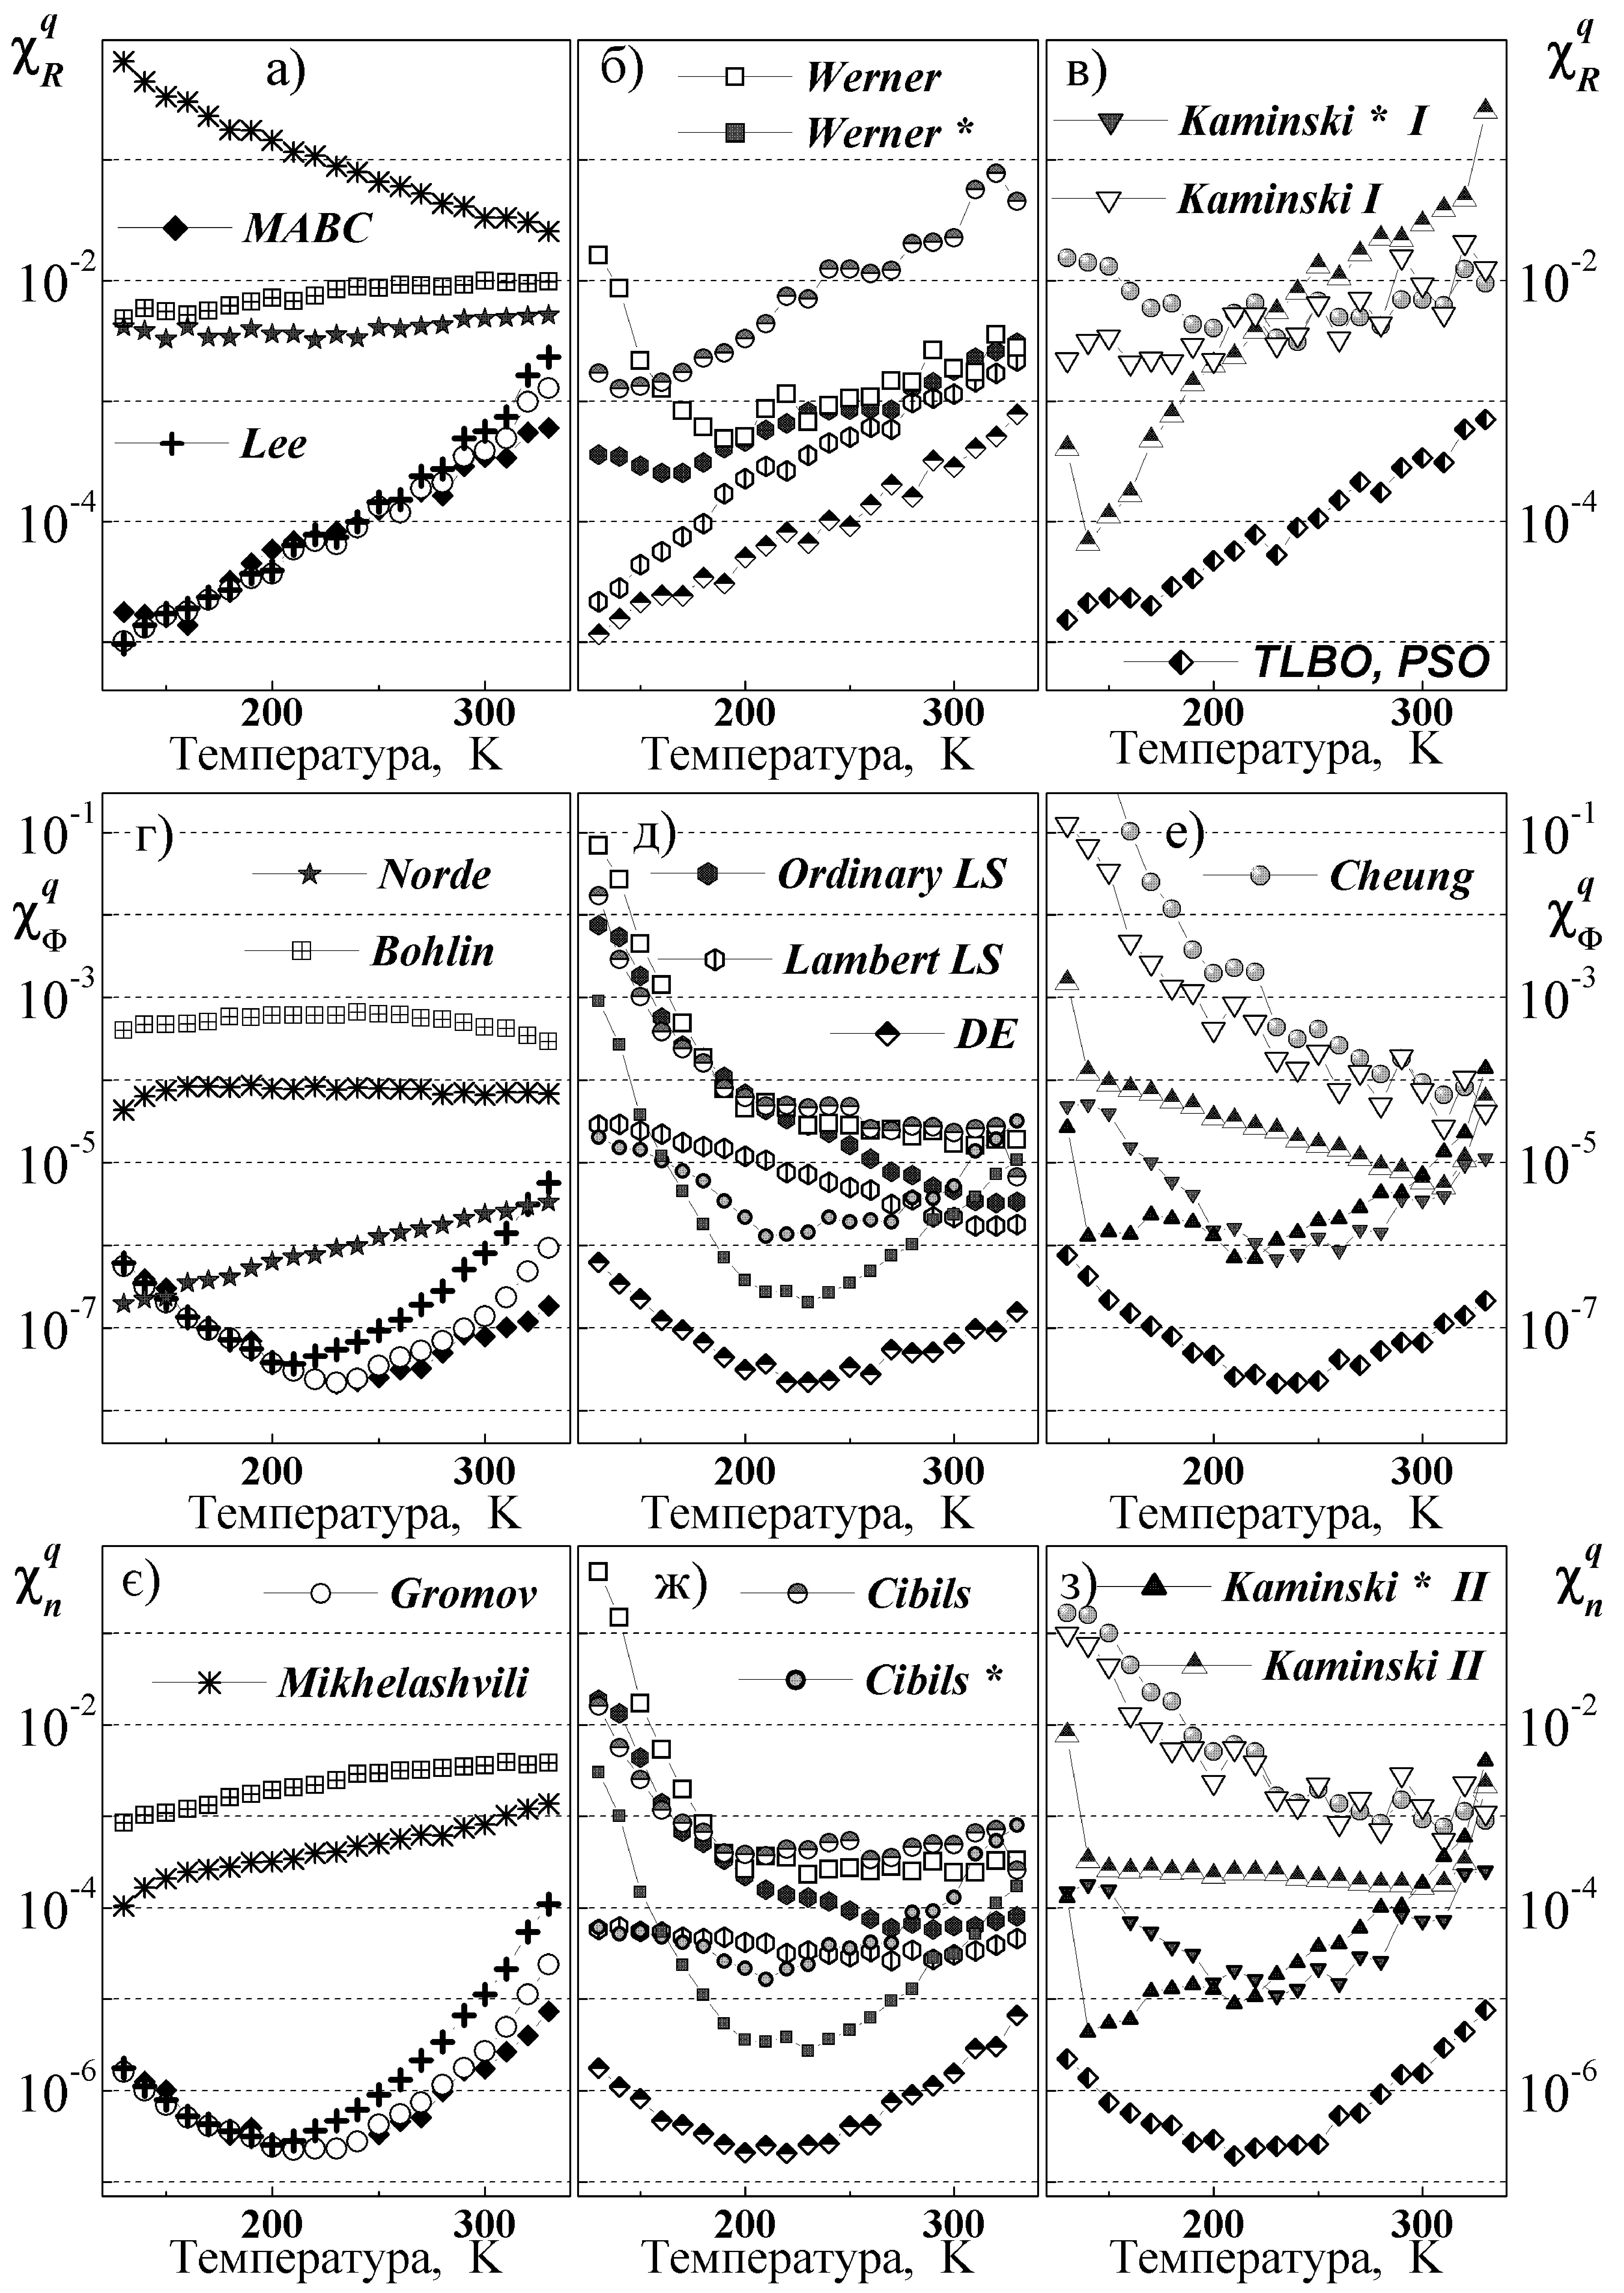
\includegraphics[width=0.8\textwidth]{figG1003}%
\caption{\label{figG1003}
Температурні залежності похибок визначення послідовного опору (а --- в), ВБШ (г --- е) та фактора неідеальності (є --- з) при застосуванні різних методів до наборів зашумлених даних.
$\sigma_V=0,3$~мВ, $\sigma_I^\varepsilon=1\%$
}
\end{figure}

\begin{figure}
\center
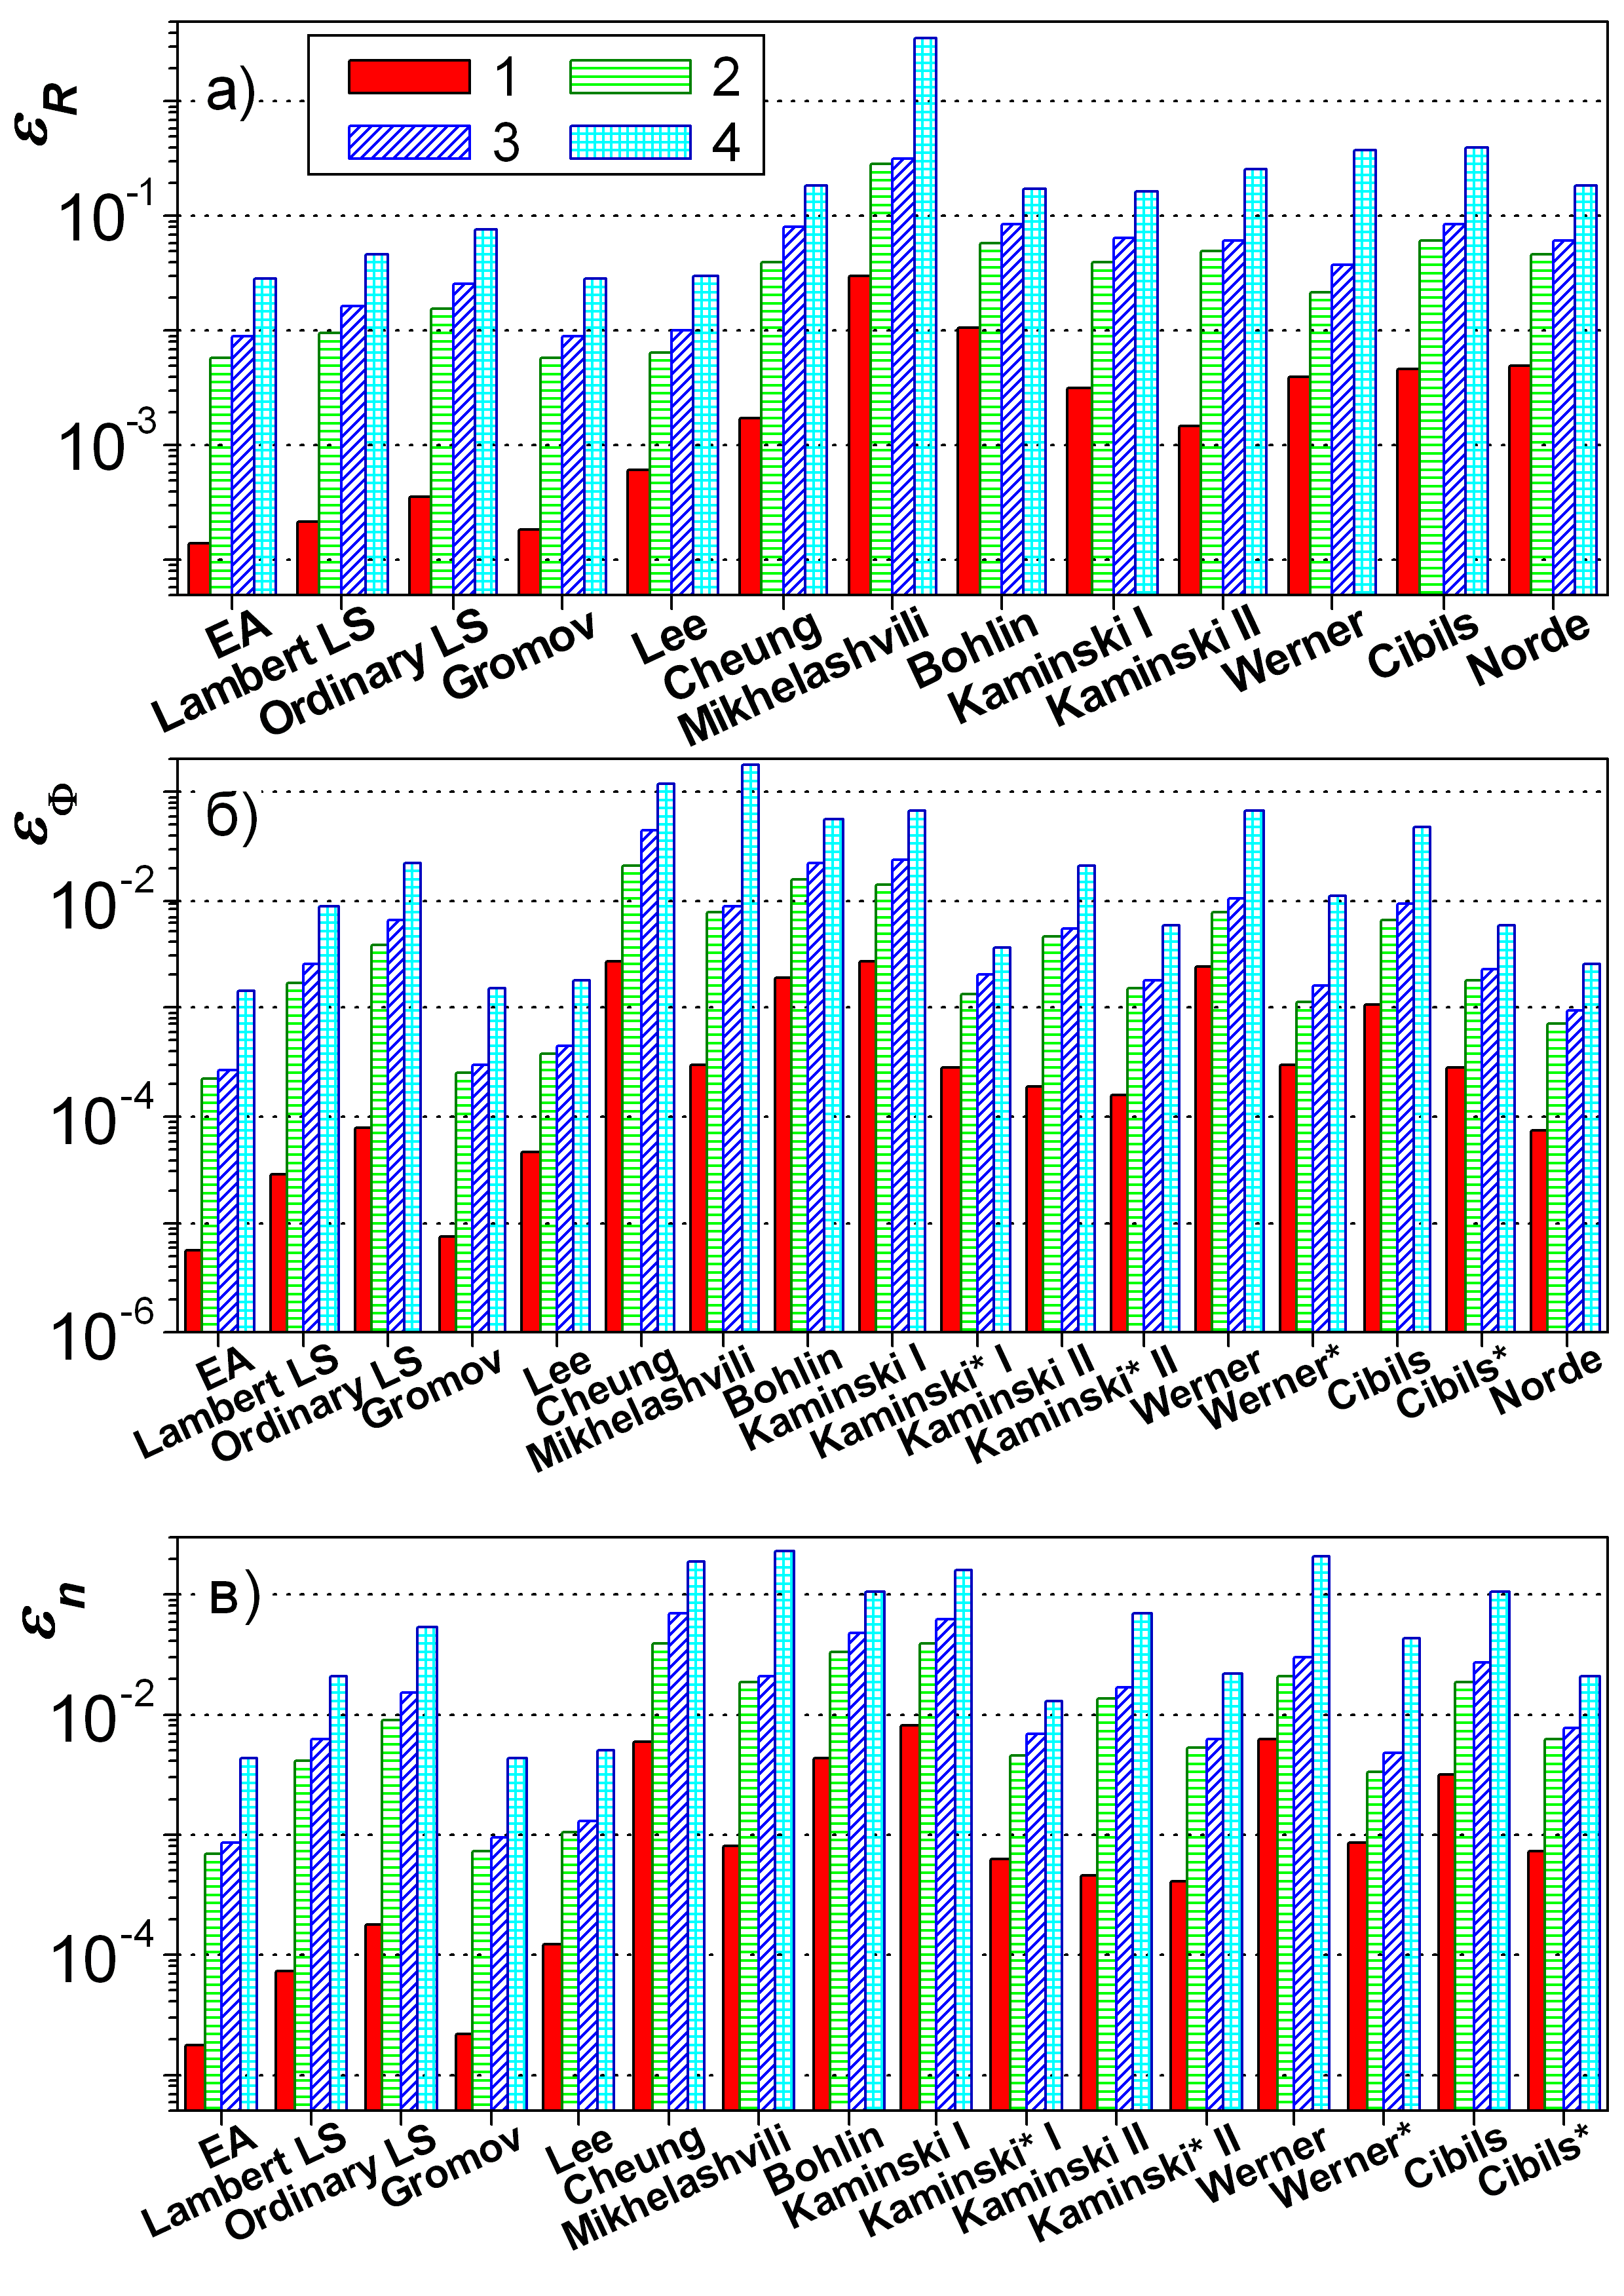
\includegraphics[width=0.8\textwidth]{figDiag}%
\caption{\label{figDiag}
Похибки визначення $R_s$ (a), $\Phi_b$ (б) та $n_\mathrm{id}$ (в) з наборів зашумлених даних.
$\sigma_V$, мВ: 0 (1), 0,3 (2, 3), 2 (4).
$\sigma_I^\varepsilon$, \%: 0 (1), 0,5 (2), 1 (3, 4)
}
\end{figure}


У випадку, коли методи Werner, Cibils, Kaminskii~I або  Kaminskii~IІ застосовуються до зашумлених даних, визначення $n_\mathrm{id}$ шляхом апроксимації скорегованої ВАХ є більш точним, ніж у випадку, коли ця величина визначається внаслідок апроксимації допоміжної функції.
Крім того, точність цих методів наближається до найкращих результатів інших методів і стає порівняною з точністю числових методів, або й навіть переважає її (рис.~\ref{figG1003}).
Метод Norde дозволяє достатньо точно визначати висоту бар'єру Шотткі, проте фактор неідеальності можна отримати лише застосовуючи інші методи.

Залежності похибок визначення параметрів від рівня шуму (від рівня випадкових помилок) показані на рис.~\ref{figErr}.
Наведені графіки отримані при використанні методу Gromov, проте вони є цілком типовими і для інших методів також.
Видно, що величини помилок при визначенні всіх параметрів практично лінійно залежать як від похибок вимірювання напруги, так і від відносних похибок сили струму.
Крім того, помилки визначення $\Phi_b$ та $n_\mathrm{id}$, викликані неточністю вимірювання напруги та сили струму, значно менші, ніж помилки визначення послідовного опору за тих самих умов.


\begin{figure}
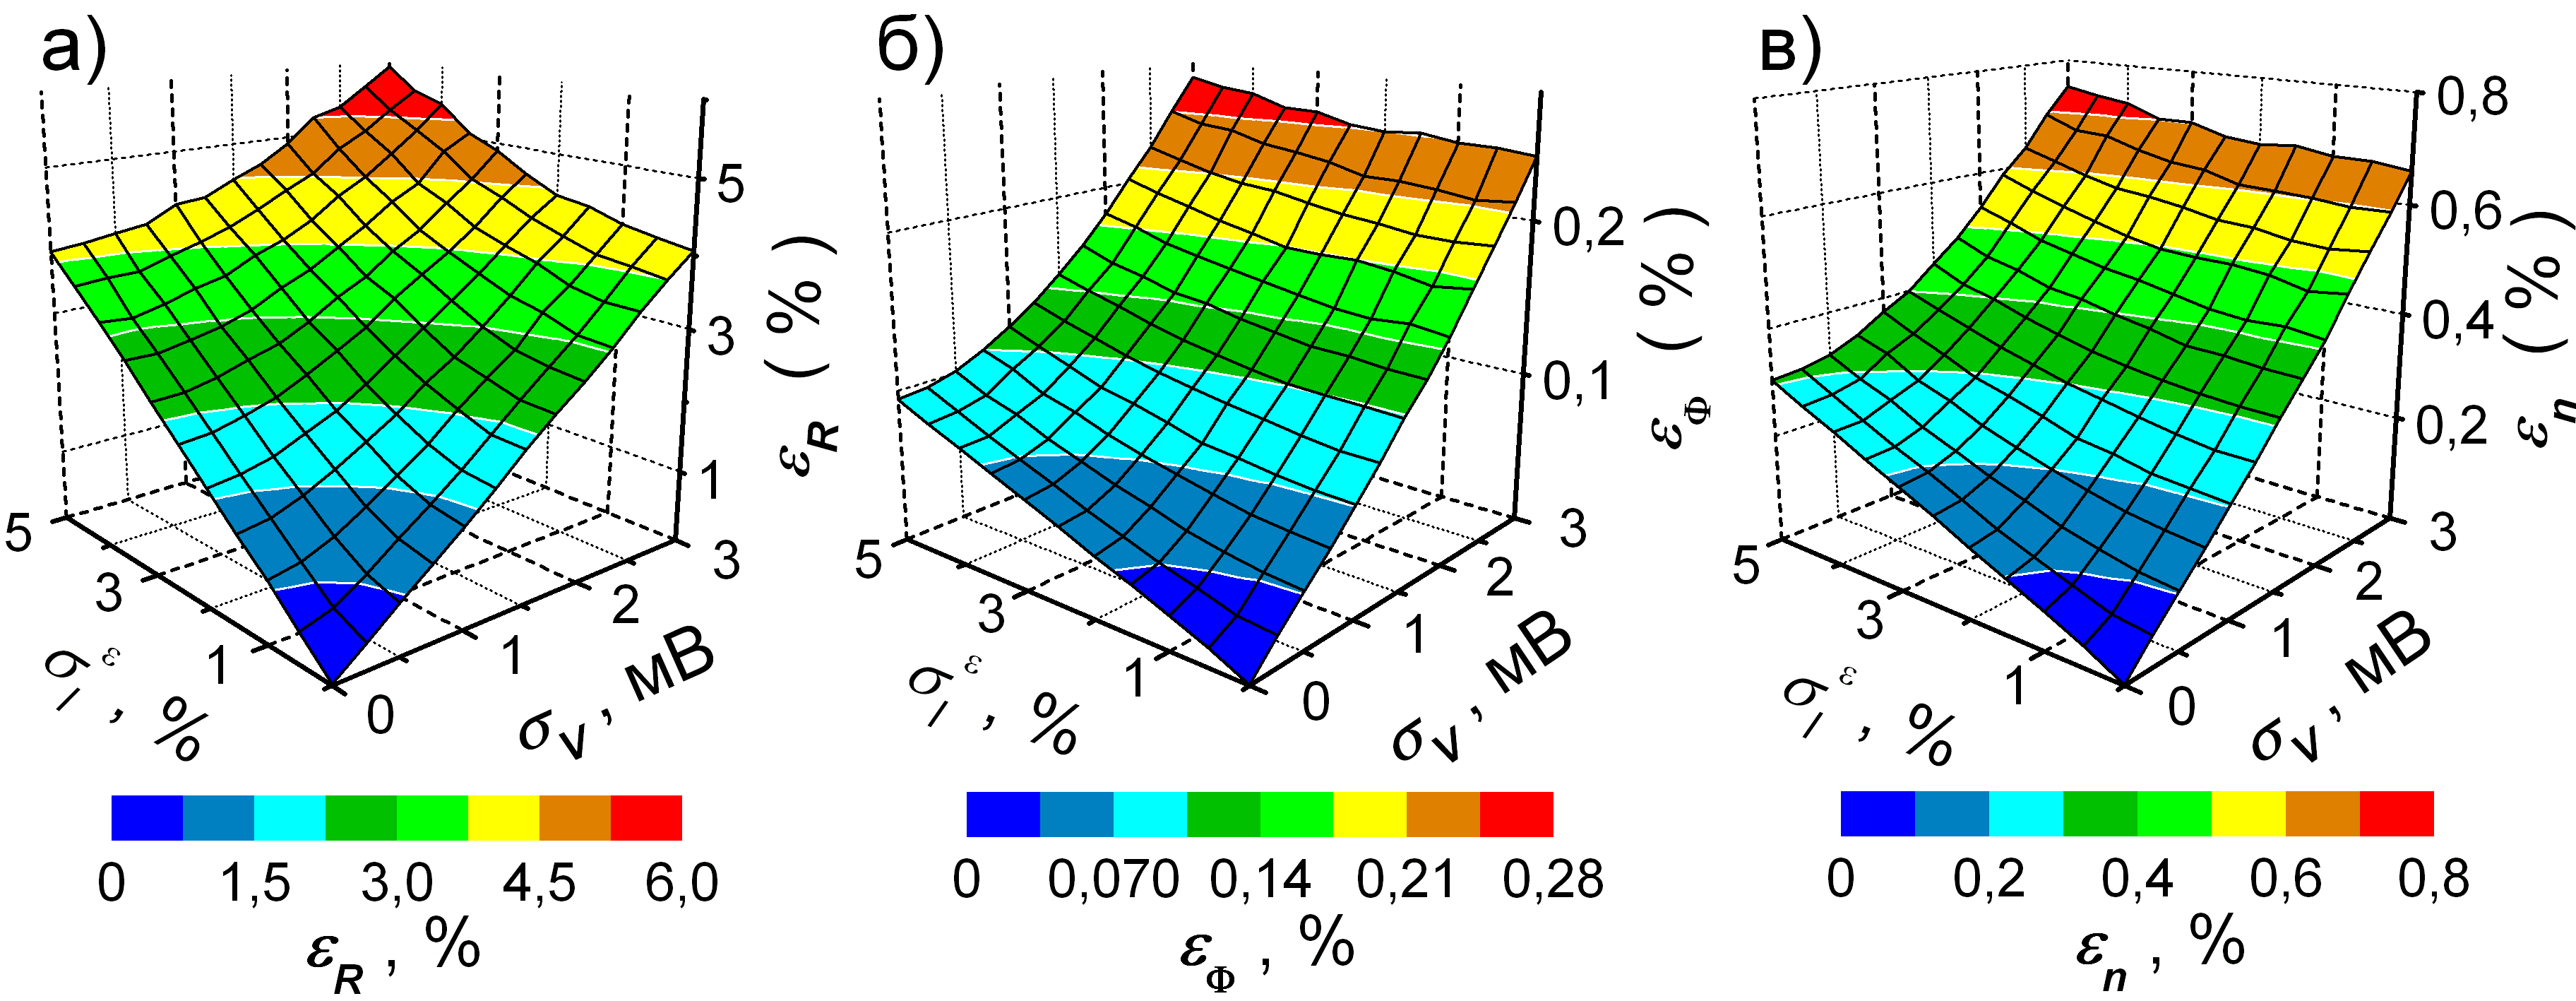
\includegraphics[width=1\textwidth]{figErr}%
\caption{\label{figErr}
Залежності похибок визначення $R_s$ (a), $\Phi_b$ (б) та $n_\mathrm{id}$ (в) при використанні методу Gromov  від похибок вимірювання сили струму та напруги
}
\end{figure}


\subsection{Визначення параметрів реальних структур метал--напівпровідник}

Температурні залежності параметрів, отриманих з експериментальних ВАХ наведені на рис.~\ref{figPract}.
Зауважимо, що в цьому випадку при застосуванні метода Bohlin були використані значення $\gamma_1=1,6$ та $\gamma_2=1,8$ замість  $\gamma_1=1,6$ та $\gamma_2=3,5$, для яких, як показано в розділі~\ref{AnMethod}, очікується менше значення похибки.
Це пов'язано з тим, що для діапазону сил струму, у якому були отримані експериментальні дані, відсутній мінімум функції Норда з $\gamma_N=3.5$.



\begin{figure}
\center
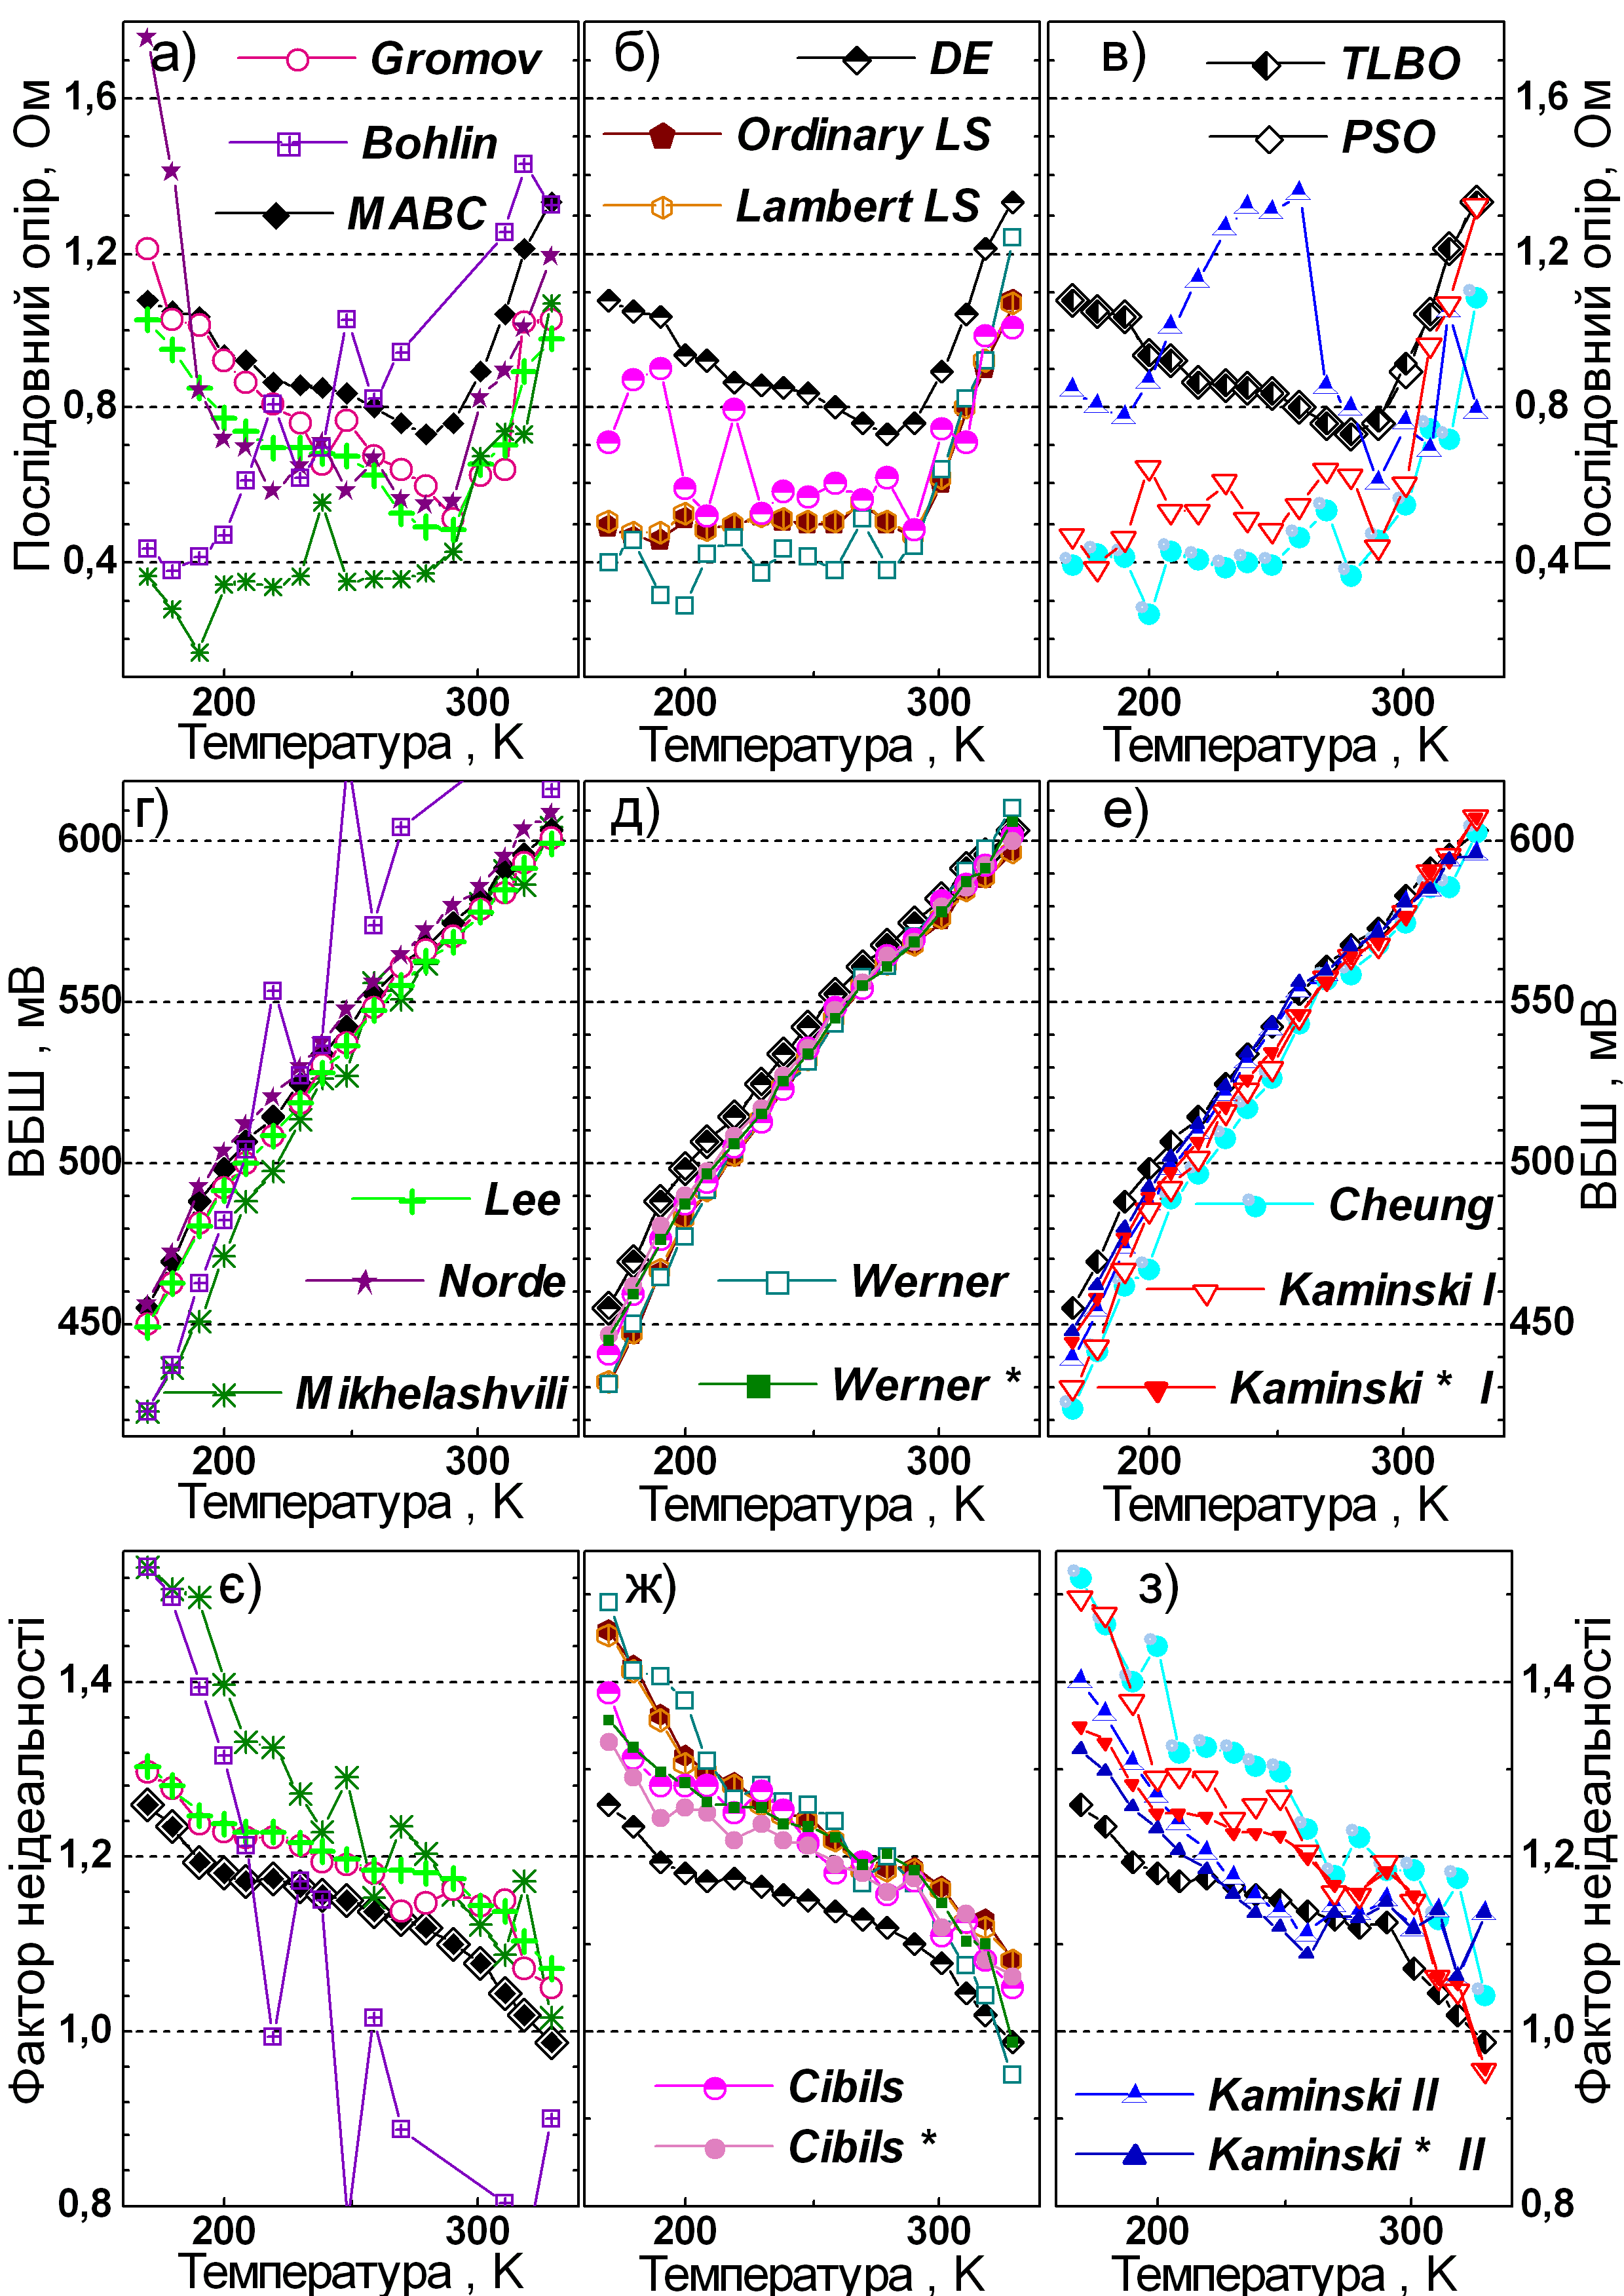
\includegraphics[width=0.8\textwidth]{figPract}%
\caption{\label{figPract}
Температурні залежності послідовного опору (а --- в), ВБШ (г --- е) та фактора неідеальності (є --- з) при
застосуванні різних методів до експериментальних ВАХ
}
\end{figure}

Виявлена температурна залежність висоти бар'єру, які відрізняється від виразу (\ref{eqFbT}), що використовувався при синтезі ВАХ, може бути пов'язана з неоднорідністю контакту МН \cite{Tung:MSE,Olikh:2013IEEE}.
Зростання послідовного опору при високих температурах в літературі \cite{Rs:Dokme} пов'язується з тим, що за цих умов визначальним для $R_s$ буде контактний опір, а не опір об'єму напівпровідника.

Зупинимось на отриманих температурних залежностях послідовного опору.
Використання ЕА, методів Gromov та Lee дозволяє виявити немонотонну температурну залежність $R_s$, причому абсолютні значення опору, отримані за допомогою різних методів, дещо відрізняються.
Взявши до уваги невелике значення послідовного опору (близько 1~Ом), а також виявлене раніше значне збільшення похибок методів Gromov та Lee при малих значеннях $R_s$ та великих $I_s$ (рис.~\ref{figId},a, \ref{figR3D},a, \ref{figR3D},б та \ref{figG1003},a), можна зробити висновок, що величини, отримані при застосуванні еволюційних алгоритмів, більш правильні.
З фізичної точки зору, виявлена поступова зміна опору з температурою є цілком ймовірною.
При застосуванні числових методів отримана залежність $R_s$ від $T$ також є досить гладкою, проте її поведінка відрізняється від результатів ЕА при низьких температурах (рис.~\ref{figPract},б).
З іншого боку, зашумленість температурних залежностей має свідчити про наявність помилок або під час вимірювань ВАХ, або під час визначення параметрів, а саме такі залежності виникають при застосуванні інших методів.

Подібні особливості характерні і для визначених залежностей ВБШ та фактора неідеальності.
Розкид значень $\Phi_b$ суттєво менший ніж для $n_\mathrm{id}$, що корелює з меншою величиною похибки визначення ВБШ (рис.~\ref{figG1003} -- \ref{figErr}).
Найбільш погані результати отримані при використанні методів Bohlin, Mikhelashvili та Cheung.

Для оцінки розходжень виміряних та апроксимуючих ВАХ було використане середнє значення відхилення сили струму $\Delta_I$:
 \begin{equation}
 \label{eqMCur}
 \Delta_I=\frac{1}{N_p}\sum_{i=1}^{N_p}\left|\frac{I_{calc}(V_i)-I_i}{I_i}\right|.
 \end{equation}
При обчисленні $\Delta_I$, значення $I_{calc}(V_i)$ розраховувалися з використанням виразів (\ref{eqSDIV}--\ref{eqSDIs}) та параметрів, визначених при використанні різних методів.
Результати для трьох ВАХ, виміряних при різних температурах, наведені на рис.~\ref{figPrAcc}.
Як видно, в цьому випадку еволюційні алгоритми, методи Gromov та Lee також продемонстрували свої переваги.


\begin{figure}
\center
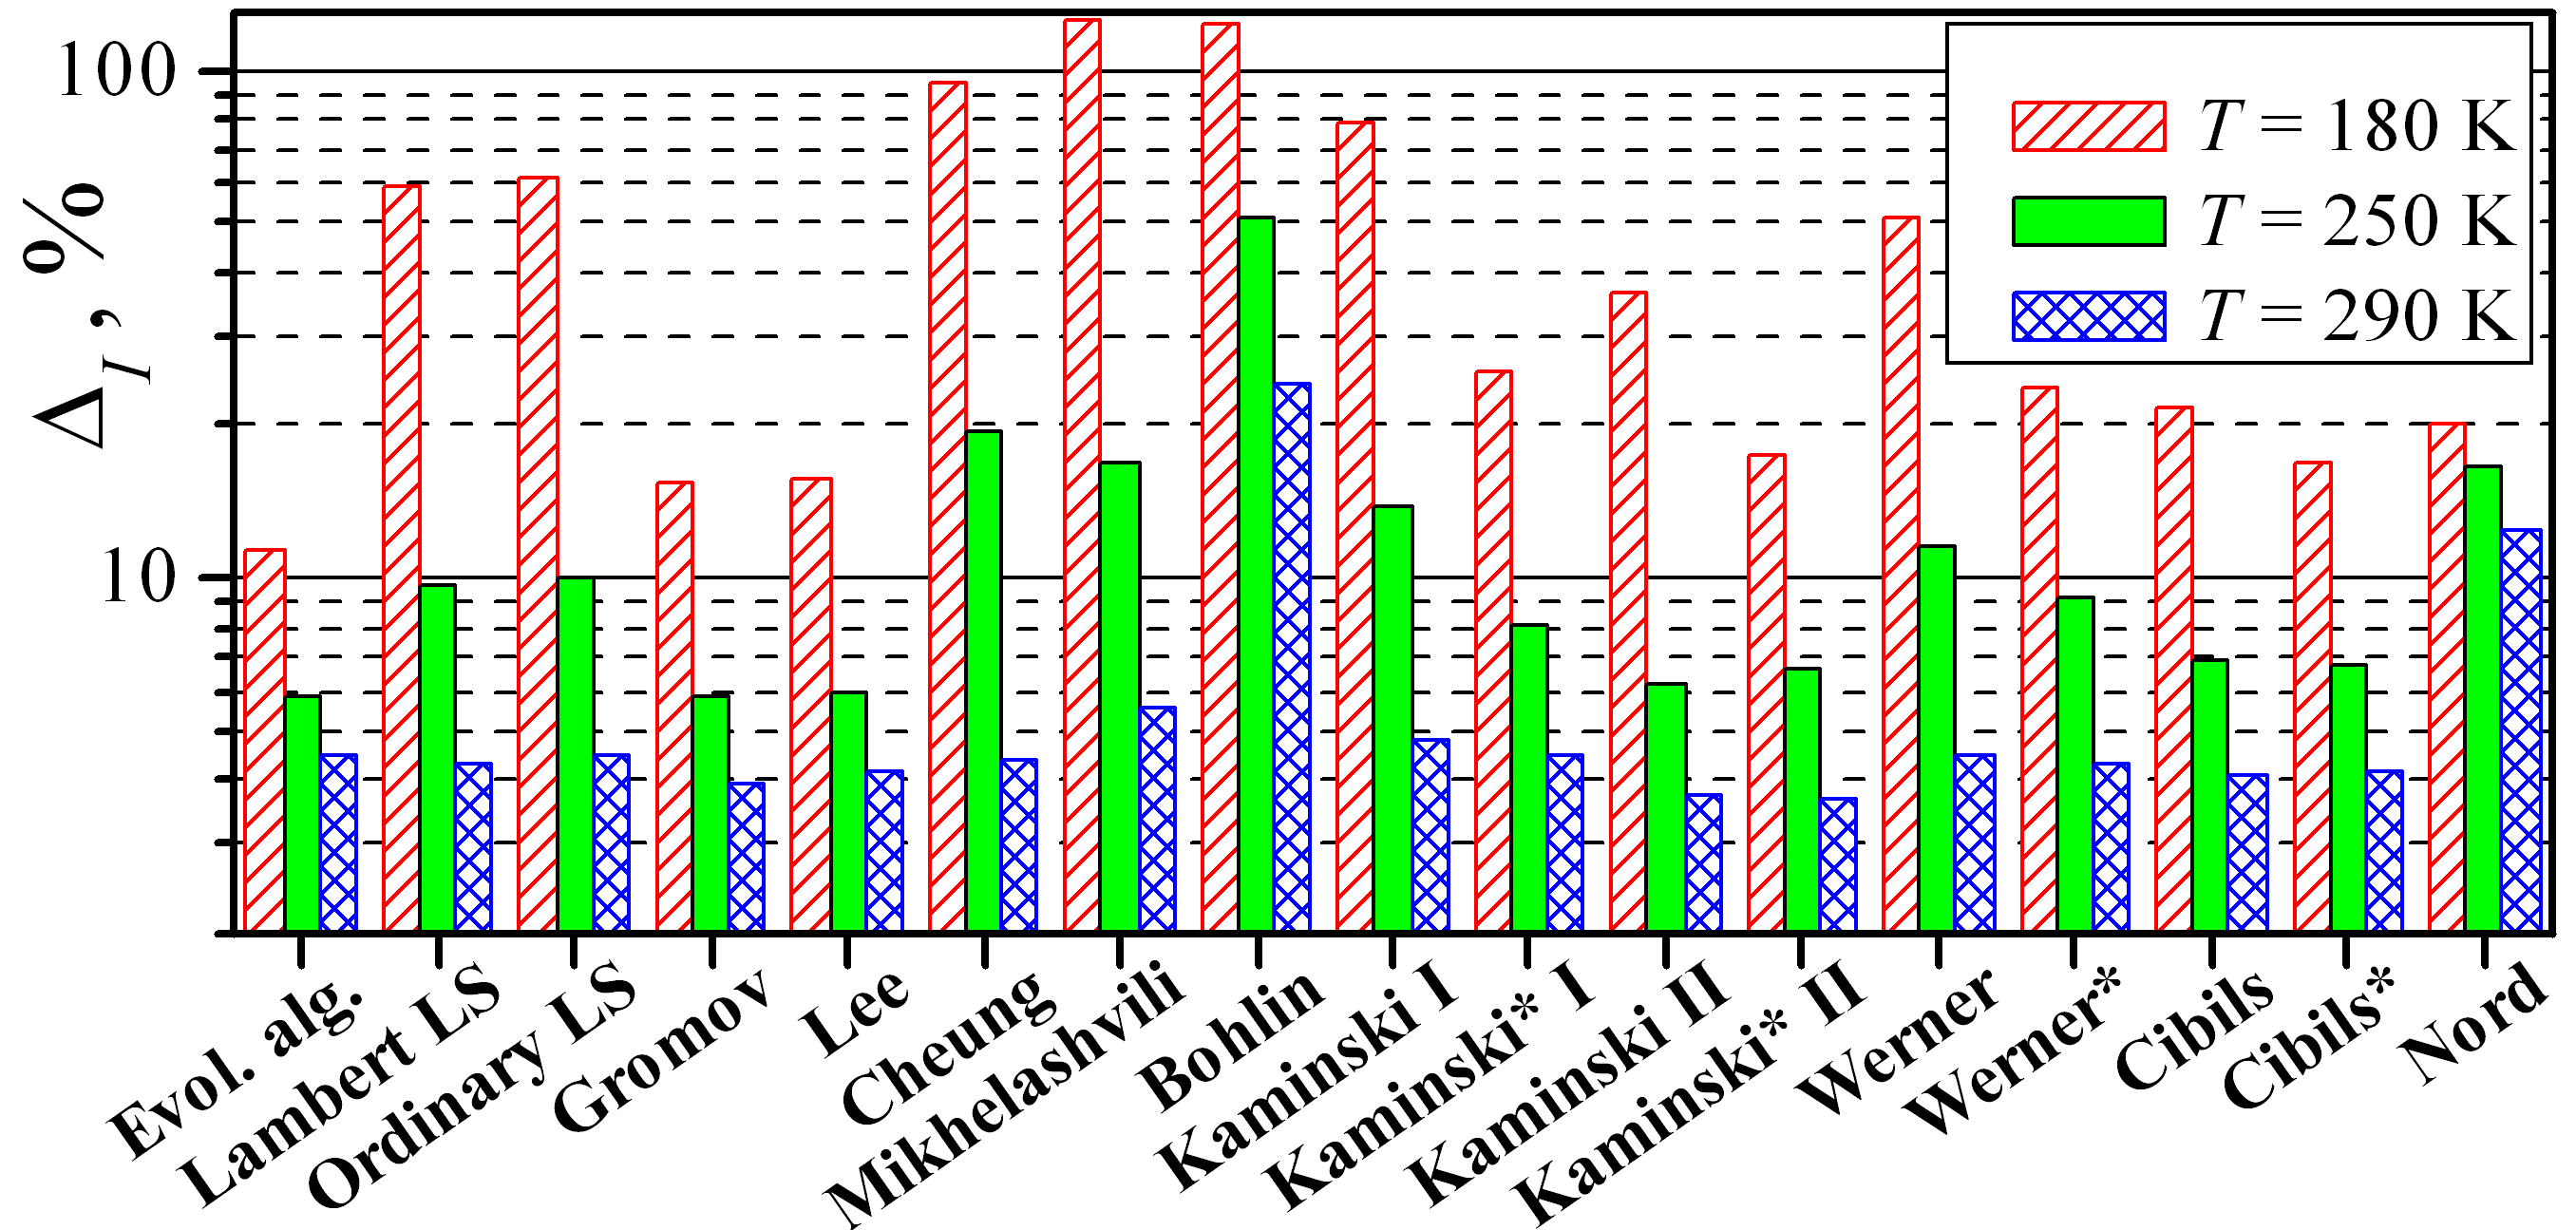
\includegraphics[width=0.8\textwidth]{figPrAcc}%
\caption{\label{figPrAcc}
Середні значення відносного відхилення розрахованих значень сили струму від експериментальних даних
}
\end{figure}

Як було сказано раніше, і експериментальні ВАХ отримані для кремнієвих структур, і при синтезі даних вважалося, що ДШ створені з використанням саме цього напівпровідника.
На мою думку, висновки щодо того, які методи є найбільш достовірними та такими, що мають перевагу, залишаються справедливими і при дослідженні структур не на основі кремнію.
Дійсно, для діодів з іншого матеріалу можуть спостерігатися зміни  величин $\Phi_b$, $n_\mathrm{id}$, $R_s$ та їх співвідношень.
Проте еволюційні алгоритми, методи Lee та Gromov з адаптивною процедурою довели свою перевагу для досить широкого діапазону значень параметрів.
З іншого боку, зміна матеріалу може викликати модифікацію
а)~температурної залежності точності визначення параметрів;
б)~абсолютного значення похибки.
Проте подібні зміни для конкретного напівпровідника можуть бути у першому наближені оцінені з використанням даних, наведених у табл.~\ref{tabIF}.

Проте необхідно підкреслити, що отримані результати будуть коректними для тих ДШ, для яких ВАХ описуються рівнянням~(\ref{eqSDIV}).
Наприклад, відхилення від цього закону характеристик реальних діодів може бути пов'язане з наявністю шунтуючого опору чи неоднорідністю бар'єру \cite{Tung:MSE,OlikhJAP}.
Проте в подібних випадках застосування еволюційних алгоритмів може суттєво спростити процедуру визначення параметрів структур МН.


\section*{Висновки до розділу \ref{Ch_MSMethod}}
\addcontentsline{toc}{section}{Висновки до розділу \ref{Ch_MSMethod}}	
  \begin{enumerate}[leftmargin=0cm,itemindent=3em]
     \item Проведено порівняльний аналіз та тестування 16 основних відомих методів визначення параметрів діодів Шотткі з вольт--амперних характеристик.
         Спираючись на результати тестування методів на експериментальних та синтезованих  ВАХ,
         запропоновано шляхи їх оптимізації з метою збільшення точності розрахунку.

     \item Для методу Норда проведено числовий аналіз залежності величин похибок визначення ВБШ та послідовного опору від величини параметра $\gamma_N$ на масиві синтезованих ідеальних та зашумлених ВАХ.
     Виявлено, що похибка визначення висоти бар'ру зростає зі збільшенням даного параметра, тоді як залежність похибки розрахунку послідовного опору є немонотонною функцією $\gamma_N$.
     Показано, що оптимальним значенням є $\gamma_N=1,8$.


     \item Проведено числовий аналіз залежності величин похибок визначення висоти бар'єру, фактора неідеальності та послідовного опору при використанні Bohlin--методу від величин параметрів $\gamma_1$ та $\gamma_2$.
     Встановлено, що в цьому методі похибка екстрагування параметрів зростає при збільшенні величини $|\gamma_1-\gamma_2|$.
     Запропоновані оптимальні (для температурного діапазону $130\div330$~К) величини $\gamma_1=1,6$ та $\gamma_2=3,5$.



     \item Для оптимізації вибору діапазону ВАХ, який використовується для побудови допоміжних функцій при застосуванні аналітичних методів визначення параметрів структур МН, запропоновано адаптивну процедуру, що базується на аналізі відхилення між апроксимуючою та експериментальною кривими.
         На прикладі аналітичного Gromov методу показано, що дана процедура дозволяє підвищити точність визначення параметрів (приблизно на порядок при кімнатних температурах у випадку низького рівня похибок вимірювання) і не викликає критичного збільшення часу, необхідного для розрахунків.

     \item Запропоновано модифікацію методу Mikhelashvili, яка дозволяє застосовувати його в автоматичному режимі до множини ВАХ.
     Вона полягає у послідовному використанні медіанного фільтру та процедури згладжування функції $\alpha(V)=d(\ln I)/d(\ln V)$ перед визначенням положення її максимуму.
     Показано доцільність застосування запропонованої процедури при опрацюванні реальних ВАХ для підвищення точності методу, що пов'язано зі можливістю визначення саме глобального екстремума.

    \item Здійснена програмна реалізація еволюційних алгоритмів  диференційної еволюції, оптимізації зграї частинок,
модифікованої штучної бджолиної сім'ї та оптимізованого викладання та навчання при вирішенні задачі визначення параметрів структур МН.
Запропоновано та показано ефективність застосування цільової функції у вигляді суми квадратів відносних похибок апроксимації кожної з точок ВАХ.
Проведено визначення необхідної кількості поколінь для збіжності кожного з алгоритмів.

   \item Показано, що серед всіх тестованих методів, найбільш придатними з точки зору точності визначення параметрів є еволюційні алгоритми (особливо MABC завдяки найменшому часу розрахунку), метод Gromov з адаптивною процедурою та метод Lee, причому ЕА дозволяють отримати найбільш коректні результати при малих (декілька Ом) значеннях послідовного опору або великих значеннях струму насичення (високих температурах).
    Показано, що використання функції Ламберта при числовому визначенні параметрів ДШ дозволяє зменшити похибки визначення та вплив на них інших факторів; з іншого боку, час роботи алгоритму зростає.
    Проаналізовано залежності точностей визначення послідовного опору, висоти бар'єру Шотткі та фактора неідельності від величин параметрів та рівня випадкових помилок вимірювання ВАХ.

  \end{enumerate}

Предсталені в даному розділі результати огляду, тестування та порівняльного аналізу методів визначення параметрів діодів Шотткі будуть корисними для подальших дослідження та розробки
МН пристроїв.

Основні результати даного розділу представлені та використані в роботах \cite{Olikh:Rev,6CPFCS,OlikhJAP,Olikh:Ultras2016,Olikh2016JSem}.
